% Tesis ITAM CLASS -- version 0.1 (13 - Abr - 2015)
% Clase para las tesis del ITAM
%% LICENSE: Creative Commons SA-BY 3.0
%
%
% Este documento presenta un ejemplo de uso de la plantilla
% El estudiante es libre de modificar este archivo a su gusto
% 
\documentclass[12pt]{tesisITAM}
\usepackage[T1]{fontenc}
\usepackage[utf8]{inputenc}
\usepackage{amsmath}
\usepackage{amssymb}
\usepackage{amsthm}
\renewcommand\qedsymbol{$\qed$}
\usepackage{mathtools}
\DeclarePairedDelimiter\ceil{\lceil}{\rceil}
\DeclarePairedDelimiter\floor{\lfloor}{\rfloor}
\usepackage{tikz}
\usepackage{algorithm}
\usepackage{algpseudocode}
\usepackage{setspace}
% \usepackage{biblatex}
\usepackage{wrapfig}
\usepackage{changepage}
\usepackage{graphicx}
% \addbibresource{references.bib}
\usepackage{natbib}
\usepackage[toc,page]{appendix}
\usetikzlibrary{decorations.markings}
\usetikzlibrary{shapes.geometric}
\usetikzlibrary{shapes,fit}

\pgfdeclarelayer{edgelayer}
\pgfdeclarelayer{nodelayer}
\pgfsetlayers{edgelayer,nodelayer,main}

\tikzstyle{none}=[inner sep=0pt]
\tikzstyle{node}=[circle,draw=black!100,fill=gray!20]
\tikzstyle{split-node}=[circle split,draw=black!100,fill=gray!20,rotate=90]
\tikzstyle{undir-edge}=[-,draw=black!100,ultra thick]
\tikzstyle{dir-edge}=[->,draw=black!100,ultra thick]
\tikzstyle{label}=[rectangle,draw=black!100,fill=white!100]
\tikzstyle{simple-label}=[rectangle,draw=white!100,fill=white!100]
\tikzstyle{label-edge}=[->,dashed,draw=black!100,thick]
\tikzstyle{dotted}=[-,dashed,draw=black!20,thick]
\tikzstyle{big-arrow}=[single arrow,draw=black,fill=black!10,minimum height=1.5cm]


%\usepackage[linesnumbered,ruled,vlined]{algorithm2e}
%\usepackage[]{algorithm2e}
%\usepackage[dotocloa,boxed,algochapter]{algorithm2e} 
\usepackage[algochapter,linesnumbered,noend,ruled,oldcommands]{algorithm2e}
\newcommand*{\field}[1]{\mathbb{#1}}%
 \usepackage{algcompatible}

\makeatletter
\renewcommand{\@chapapp}{}% Not necessary...
\newenvironment{chapquote}[2][2em]
  {\setlength{\@tempdima}{#1}%
   \def\chapquote@author{#2}%
   \parshape 1 \@tempdima \dimexpr\textwidth-2\@tempdima\relax%
   \itshape}
  {\par\normalfont\hfill--\ \chapquote@author\hspace*{\@tempdima}\par\bigskip}
\makeatother


\title{Análisis de la estructura de redes sociales con modelos de redes aleatorias exponenciales}
\author{Patricio Dávila Barberena}
\degree{Licenciado en Matemáticas Aplicadas}
\advisor{Dr. Juan José Fernández Durán}
\year{2019}

\newtheorem{definition}{Definición}[chapter]
\newtheorem{theorem}{Teorema}[chapter]
\newtheorem{corollary}{Corolario}[chapter]
\newtheorem{example}{Ejemplo}[chapter]

\begin{document}

	\pagenumbering{gobble}
	\maketitle
	\publicationrights
    
    \cleardoublepage
    \chapter*{Agradecimientos}
Quiero agradecer a mi madre, Yolanda Barberena, y a mi padre, Antonio Dávila, por apoyarme incondicionalmente en todas mis decisiones a pesar de su mejor juicio. A mis hermanos Tony y Luis por ser los mejores guías y navegadores de este océano de vida. Al resto de mi familia por estar presentes en mi vida.

Me gustaría agradecer a mis camaradas matemáticos, Roberto Ortiz, Adrián Tamecito, Ilan Jinich, Santiago Córdoba y muchos más porque sin ellos no habría podido abrirme camino a través de la universidad como lo hice. Espero crecer aún más al lado de ellos. Nunca nos van a hacer falta las risas. Somos parte de la mejor generación.

También me gustaría agradecer a Lukas Canal, Eduardo Carbia y Angel Hernández, cofundadores de Hexagon Data, por permitirme la libertad de usar algunos de los datos utilizados en esta tesis y por su flexibilidad que me permitió trabajar y estudiar simultáneamente.

Finalmente, me gustaría agradecer a mi asesor, Juan José Fernández Durán, por poder entender perfectamente e inmediatamente cuáles eran el propósito y los objetivos de mi tesis.

\clearpage



	%%%%%%%%%%%%%%%%%%%%%%%%%%%%%%%%%%%%%%%%%%%%%%
	% ABSTRACT
	%%%%%%%%%%%%%%%%%%%%%%%%%%%%%%%%%%%%%%%%%%%%%%

	\begin{abstract}{spanish}
	En este trabajo se profundiza sobre los modelos de grafos aleatorios exponenciales. Se utiliza este enfoque para la predicción de la estructura de los grafos en el siguiente momento del tiempo y se interpretan los resultados de la estimación de los parámetros que están asociados a esta estructura. Además, se hace el análisis de varias redes sociales con el fin de describirlas y de detectar las comunidades subyacentes en está al igual que predecir su siguiente estado.
	\end{abstract}
  
%	\begin{abstract}{english}
%		In this work we present a template for thesis and titulation works presented at ITAM. It is provided freely and without any responsability under the \emph{creative commons BY-SA 3.0}. 
%	\end{abstract}

    \cleardoublepage
    \selectlanguage{spanish}
	\setcounter{page}{1}
	\pagenumbering{roman}

	\tableofcontents
    
	\cleardoublepage
    \phantomsection
    \addcontentsline{toc}{chapter}{\listfigurename}
	\listoffigures
	\newpage
    
    %\listoftodos
    %\todo{eliminar lista de TODO}

	\cleardoublepage
	\pagenumbering{arabic}
	\setcounter{page}{1}

	%%%%%%%%%%%%%%%%%%%%%%%%%%%%%%%%%%%%%%%%%%%%%%
	% CONTENT
	%%%%%%%%%%%%%%%%%%%%%%%%%%%%%%%%%%%%%%%%%%%%%%
    
    \chapter{Introducción}


\begin{wrapfigure}{r}{.5\textwidth}
    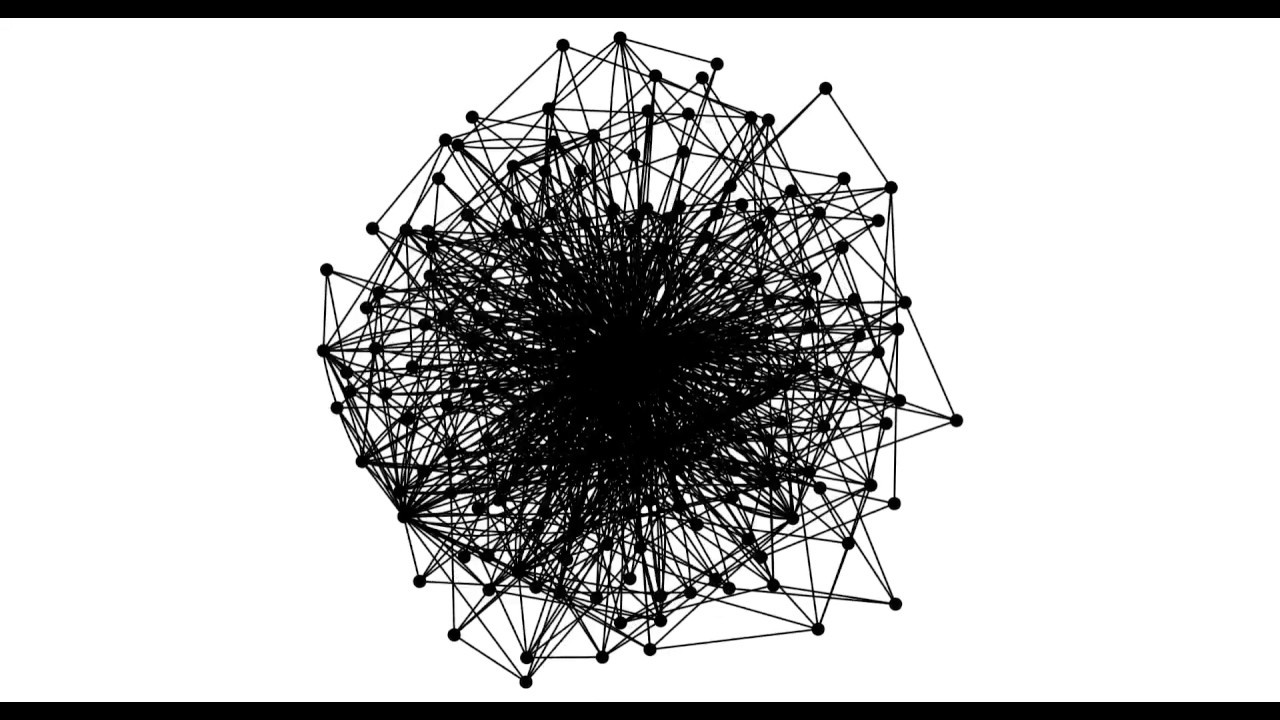
\includegraphics[width=.5\textwidth]{Tesis/Figures/smallworld.jpg}
    \caption{Gráfica del mundo pequeño con 500 nodos}
\end{wrapfigure}

Los grafos son objetos compuestos de cosas y las relaciones entre ellas. Los nodos de un grafo representan entidades mientras que las aristas son cualquier tipo de interacción o conexión entre las entidades. Existen una variedad de tipos de grafos, desde grafos sociales, grafos de colaboración, grafos financieros y muchos más. Las representaciones visuales de los grafos tienden a ser un poco confusas pues sólo son líneas conectando círculos y conforme crece el número de elementos se vuelven aún más confusas.

Sin embargo, sabemos que las interacciones entre las entidades, sean personas o bancos, rara vez se dan de forma aleatoria. Las motivaciones para la creación de una relación entre entidades no puede observarse directamente a partir de las aristas en un grafo ni tampoco se pueden deducir ojeando la base de datos que contenga los datos relacionales. Sin embargo, en nuestro repertorio de herramientas se encuentran diversas técnicas de análisis matemático que nos permiten hacer un análisis más completo de los grafos. En esta tesis se va a plantear el marco teórico de los modelos de grafos aleatorios exponenciales (ERGMs) que son un tipo de regresión logística modificada que permiten calcular la probabilidad de que exista una arista dado la presencia de otras aristas dentro de un grafo.


\section{Antecedentes}

Las grafos sociales impregnan nuestra vida social y económica pues juegan un papel central en comunicar oportunidades de trabajo, estatus social, información sobre el mundo y son críticas para el funcionamiento del mundo digital. Las grafos sociales también son importantes para predecir cómo se esparcen las enfermedades, qué productos son populares, qué lenguas se hablan y además repercuten en la forma en la que participamos en nuestras democracias. Es por todas estas razones que si queremos entender el mundo y hacerlo más próspero debemos de entender las estructuras fundamentales de las grafos y de qué forma se presentan en nuestra sociedad.

El propósito de esta tesis es proporcionar un marco teórico para el análisis de las grafos manteniendo en mente el importante aspecto social.

Por mucho tiempo ha sido de interés para los matemáticos encontrar formas para describir las características de una red observada. Estas grafos se han presentando en nuestras estructuras sociales desde el inicio del tiempo sea a través de las grafos sociales de amigos, las grafos de comercio, las grafos de influencia y muchas otras más. En particular desde la apertura del internet, que conlleva el registro de nuestras actividades humanas en bases de datos digitales, la disponibilidad de bases de datos de estas grafos se ha disparado.

Las actividades de usuarios en internet pueden ser registradas con gran detalle. Este monitoreo está presente a través de casi todas las plataformas que crean contenido y existen un gran número de distintas implementaciones para monitorear el comportamiento de los usuarios en estas mismas plataformas. A través del tiempo las empresas han acumulado mucha información sobre sus usuarios con la meta de comprender a sus audiencias. Por ejemplo, si un usuario a menudo consume cierto tipo de contenido entonces este mismo usuario es más probable que esté interesado en ese tipo de contenido en el futuro. Entonces, al monitorear las actividades de los usuarios es que se puede crear una representación del tipo de contenido consumido por los usuarios y se pueden generar modelos para recomendarle contenido relevante a todos.


Grandes empresas han dedicado muchos recursos al modelaje del comportamiento de sus usuarios como Facebook, Linkedin, Netflix y Amazon. Sin embargo, la información recopilada de los usuarios de una sola plataforma puede estar sesgada pues los usuarios en realidad pueden consumir distintos tipos de contenido de distintas páginas. Sin embargo, existen varias soluciones a este problema de seguir a los usuarios en las distintas plataformas en las que consumen contenido. Para conseguir una mejor representación de las preferencias de un usuario cualquiera se han utilizado \textit{cookies} anónimas en donde la tecnología de sincronización juega un rol esencial. Esta tecnología permite el rastreo de las acciones registradas en un buscador de internet.

Cuando un usuario visita un sitio el proveedor del contenido genera una \textit{cookie} que está atada al buscador del usuario. Entonces, el proveedor de contenido \textit{hashea} la clave del usuario y la registra en una base de datos de un proveedor de servicios estratégicos, como un \textit{Data Management Platform (DMP)}. Además en ese mismo momento se registra el tipo de comportamiento del usuario en una base de datos y el usuario se le asigna una audiencia en un mercado de audiencias en el cual cualquier tercero puede añadir esos usuarios anónimos a sus audiencias. Los terceros por su parte se comprometen a registrar el comportamiento de los usuarios de sus propiedades digitales y lo suben a la misma base. Las empresas pueden también utilizar sus bases de datos \textit{offline}, como el registro de compras de un \textit{ecommerce}  y asignarle una clave única a cada usuario para después cruzar los datos \textit{offline} con los comportamientos registrados en línea. A esto se le conoce como \textit{cookie syncing} y permite atar los datos que se generan en línea con aquellos que se registran a nivel físico y comercial.

Las empresas pueden generar enormes conocimientos sobre sus usuarios a partir de este tipo de prácticas de recolección de datos. De hecho existen casos extremos en donde las empresas a partir del perfil de consumidor que generaron de sus clientes pueden predecir cosas sobre sus clientes antes que ellos mismos. Un caso pronunciado de esto fue cuando un padre se entero que su hija estaba embarazada por \textit{Target} antes de que ella misma supiera. 

Estas bases de datos de usuarios anónimos son particularmente valiosas para los departamentos de marketing en las empresas y su venta representa una importante fuente de ingresos para las empresas que generan información sobre sus usuarios. Estas bases de datos de terceros permiten la implementación de la publicidad dirigida que se ha vuelto cotidiana en nuestra navegación en internet.

\section{Filtros Colaborativos}

Una de las implementaciones de modelos más famosas y útiles que han utilizado las bases de grafos se les conoce como filtros colaborativos. La idea esencial detrás de este modelo es que podemos utilizar las preferencias de usuarios parecidos entre sí para recomendar contenido. Es decir que utilizamos la información sobre miembros parecidos para hacer inferencias sobre un consumidor cualquiera.

Uno de los casos más exitosos y uno de los más personalmente importantes para mí es aquel de \textit{Spotify}, en donde se utilizan los filtros colaborativos para darle vida a uno de los principales diferenciadores de la empresa en el competitivo ámbito del \textit{streaming} de música: \textit{Spotify weekly}. La idea principal de lo que se hace en \textit{Spotify} viene ilustrada en la siguientes páginas. La idea es simple, si muchos usuarios escuchan las canciones $x,y,z$ entonces esas canciones probablemente son similares. Además si muchos usuarios escuchan las canciones $x,y,z$ y un usuario escucha las canciones $x$ y $y$ entonces deberíamos de recomendarle escuchar la canción $z$.

Todo empieza con el registro de todos los usuarios de \textit{Spotify} en donde cada usuario $u_j$ tiene asignadas las canciones $i_j$ que escuchó a un momento $t_k$:

$$\begin{array} { l } { \left( u _ { 1 } , i _ { 1 } , t _ { k } \right) } \\ { \left( u _ { 2 } , i _ { 2 } , t _ { k } \right) } \\ { \cdots } \\ { \left( u _ { n } , i _ { n } , t _ { k } \right) } \end{array}$$

Sin embargo esta representación es un poco difícil de interpretar, entonces lo que se hace es que se agregan los datos y expresamos los datos temporales en una matriz pues no importa si es que el usuario escuchó una canción una vez hace una semana y 11 veces ayer o si la escuchó 12 veces ayer si queremos saber cuáles canciones escuchó en la semana. Entonces se pueden representar todos los datos en una matriz de la siguiente forma:


$$N = \underbrace { \left( \begin{array} { c c c c } { c _ { 11 } } & { c _ { 12 } } & { \dots } & { c _ { 1 n } } \\ { c _ { 21 } } & { c _ { 22 } } & { \dots } & { c _ { 2 n } } \\ { \vdots } & { } & { } & { \vdots } \\ { c _ { m 1 } } & { c _ { m 2 } } & { \dots } & { c _ { m n } } \end{array} \right) } _ { \text {Canciones en Spotify } } \} \text { Usuarios en Spotify}$$



En esta matriz cada renglón representa un usuario y cada columna representa una canción en la biblioteca de \textit{Spotify}. Los elementos de la matriz $c_{ ij }$ son números enteros que representan la cantidad de veces que el usuario i escuchó la canción j. Esta gigantesca matriz con alrededor de $10^7 \times 10^7$ elementos tiene muchos problemas además de su enorme tamaño pues tiene muchos elementos iguales a cero (que dificultan el aprendizaje no supervisado) y muchos elementos desconocidos en caso de que se use para un problema de aprendizaje supervisado y además en realidad no necesariamente representa información verídica sobre los gustos de las personas pues las personas pueden escuchar canciones en modo \textit{offline} o de otras personas. En general es bastante difícil trabajar con esta matriz, afortunadamente los matemáticos en \textit{Spotify} son capaces de encontrar muchas formas de extraerle significado.

Por ejemplo se puede llevar a cabo el análisis entre columnas utilizando una medida de correlación como Pearson para ver qué tan similares son las columnas como en

$$c _ { i j } = \frac { \sum _ { u } N _ { u i } N _ { u j } } { \sqrt { \sum _ { u } N _ { u i } ^ { 2 } } \sqrt { \sum _ { u } N _ { u j } ^ { 2 } } }.$$

De hecho es así como \textit{Amazon} arroja las recomendaciones de productos cuando nos dice que los ``usuarios que compraron esto también compraron…''. Sin embargo la paralelización de esto es difícil pues el numerador en esa expresión es bastante denso aún cuando se tienen matrices pequeñas como

$$N = \left( \begin{array} { c c c c } { 0 } & { 7 } & { 21 } & { 0 } \\ { 5 } & { 0 } & { 0 } & { 1 } \\ { 4 } & { 0 } & { 13 } & { 9 } \\ { 0 } & { 0 } & { 0 } & { 7 } \\ { 19 } & { 1 } & { 0 } & { 13 } \\ { 0 } & { 3 } & { 0 } & { 0 } \end{array} \right)$$

En donde tendríamos que calcular 

$$N ^ { T } N = \left( \begin{array} { c c c c } { 402 } & { 19 } & { 52 } & { 288 } \\ { 19 } & { 59 } & { 147 } & { 13 } \\ { 52 } & { 147 } & { 610 } & { 117 } \\ { 288 } & { 13 } & { 117 } & { 300 } \end{array} \right)$$


Para calcular la correlación entre usuario o canciones.

Existen otras formas para utilizar esta matriz de forma más conveniente, por ejemplo lo que se llama \textit{Probabilistic Latent Semantic Analysis (PLSA)} en donde la idea es que queremos calcular las probabilidades del siguiente evento descomponiendo la matriz de tal forma que tengamos vectores de usuarios y vectores de canciones. Este es el algoritmo que de hecho se implementó dentro de \textit{Spotify} pero su explicación a detalle está fuera del alcance de esta tesis.

Fue en el transcurso de aprender más sobre la implementación de los distintos algoritmos de recomendación que empecé a trabajar en Hexagon Data, una empresa que se dedica al marketing digital, donde se me abrieron las puertas a una enorme base de datos en donde se registraban el 1\% de todas las actividades en internet. Con esta base de datos en mis manos y con las ganas de innovar es que decidí enfrentar el problema de la recomendación para descubrir conglomerados de contenido y generar audiencias de forma automatizada.


\section{Objetivo}

El objetivo de esta tesis es describir y proveer un marco teórico para el modelaje de grafos, la exploración de los modelos exponenciales, la introducción a las grafos aleatorias exponenciales, describir a las grafos sociales a través de estadísticas y proponer la implementación de un modelo de grafos aleatorias exponenciales para la utilización en la predicción del estado futuro de una red de preferencias entre usuarios y contenido a partir de la estadísticas extraídas de sus características. 


\section{Alcance}

Los modelos aleatorios de grafos exponenciales resultan bastante útiles en la descripción de las grafos sociales pues se extraen los valores de los parámetros a estimar que pueden estar asociadas a triadas u otras medidas cuya naturaleza depende de la interacción entre los nodos de la red. Es decir que el modelo permite incorporar elementos de probabilidad condicional cuando se hace la predicción del futuro de la red. Esto es consistente con el razonamiento que las personas que están interesadas en algún tipo de contenido en particular son más propensas a estar interesadas en ese tipo de contenido en el futuro. De otra forma es que si muchas personas hacen $x, y$ y $z$, entonces $x, y$ y $z$ son probablemente similares. También se puede esperar que los subgrafos de nodos que están altamente conectados seguirán estando conectados en el futuro.

Existen muchas preguntas respecto al análisis de grafos sociales que tienen que ver con el enigma de cómo es que procesos y estructuras sociales locales contribuyen a la estructura global de un grafo y si es que estos procesos locales son suficientes para explicar las preguntas que tenemos de nuestro modelo. Las realizaciones que resultan de las combinaciones de muchos procesos locales no son generalmente intuitivas, ni siquiera de forma cuantitativa. 

Posiblemente podemos navegar estos difíciles problemas con el uso de la simulación. Sin embargo, es importante tener en mente que nuestra observación de un grafo en realidad es únicamente una posible configuración de un conjunto de posibles grafos que tienen  características similares y, aunque el número de actores sea conocido, en realidad es el producto de un proceso estocástico desconocido.

Es justo nuestro enorme interés en registrar las interacciones entre los actores lo que hace la estimación de la red en el futuro particularmente difícil. Esto es porque las relaciones generalmente no son independientes y sólo podemos observar a la Grafo en un momento en el tiempo (un momento antes del futuro) y como veremos más adelante los estimadores de máxima verosimilitud de las grafos exponenciales muchas veces son desconocidos y aunque no lo fueran es computacionalmente demandante trabajar con ellos. Como veremos más adelante se utilizarán los estimadores de máxima pseudo verosimilitud que se obtienen a través del cálculo de las probabilidades condicionales completas. El teorema de Hammersley-Clifford que será demostrado más adelante forma los cimientos del marco teórico en el cual esta tesis se basa.

Los modelos de grafos exponenciales aleatorias intentan contestar al tipo de preguntas incómodas como ¿Es más probable que la gente se asocie con los amigos de sus amigos? ¿Las personas son menos propensas a asociarse con personas de distintas clases sociales? Estas preguntas se pueden intentar contestar a partir de las estructuras sociales que conforman nuestras vidas. Estos modelos generan conclusiones sobre nuestras formas de aprendizaje, la desigualdad, la propensidad a la innovación de distintas estructuras sociales y mucho más.

    
    \cleardoublepage
    \chapter{Grafos}
\label{ch:preliminaries}

\section{Tipos de Grafos}

En general existen los grafos dirigidos y no dirigidos.\footnote{Para efectos de esta tesis todos los grafos son grafos no dirigidos.}


\begin{definition}[Grafo no dirigido]
\label{grafo_def}
Un \textbf{grafo no dirigido} es una pareja ordenada $ G = (\mathcal{N}, \mathcal{E})$, en donde $\mathcal{N}$ es un conjunto finito no vacío cuyos elementos son vértices y $\mathcal{E}$ es un conjunto de subconjuntos no ordenados de cardinalidad $2$ de elementos de $\mathcal{N}$.  Estos son llamados \textbf{aristas}. 

\end{definition}

En la literatura estadística G está definido en términos de nodos y las correspondientes medidas en pares de nodos $G \equiv G ( \mathcal { N } , \mathcal { Y } )$ donde $\mathcal{Y}$ es una matriz cuadrada de tamaño $N \times N$. Esta matriz $\mathcal{Y}$ puede ser representada como una matriz de adyacencia con elementos binarios donde solo nos interesa la conexión entre nodos. Para las grafos no dirigidas la matriz $\mathcal{Y}$ es simétrica. 

Además vale la pena notar que la suma de todos los elementos de la matriz de adyacencia es 2 veces la cardinalidad del conjunto de aristas. $\sum _I \mathcal{Y}_{I} = 2E$. Los nodos del grafo podrían representar individuos, organizaciones o cualquier tipo de entidad que tenga características. Las aristas podrían representar conexiones, interacciones o relaciones que comparten las entidades.

\textbf{¿Cómo representar una red social?}

Los nodos pueden ser referidos como vértices, individuos o agentes. Estos nodos deben de ser agentes con características que comparten entre sí para poder representar sus conexiones relevantes a través de aristas.


\begin{definition}[Matriz de adyacencia]
Una \textbf{matriz de adyacencia} es una matriz cuadrada utilizada para representar un grafo finito. Los elementos $ij$ de la matriz indican si los pares de vértices $i$ y $j$ son adyacentes o no en el grafo.

\end{definition}

Visualmente podemos representar un grafo $G \equiv G ( \mathcal { N } , \mathcal { E } )$ poniendo en el plano un círculo para cada elemento de $\mathcal{N}$ con su respectiva etiqueta. A estos círculos se les llama comúnmente vértices o nodos del grafo. Para representar al conjunto de aristas del grafo unimos con un segmento de recta dos círculos si la pareja formada por sus respectivos elementos de $\mathcal{N}$ está en $\mathcal{E}$. La figura ~\ref{fig:undir-graph} muestra un ejemplo de un grafo.

\begin{figure}
\centering
\begin{tikzpicture}[scale=1.2]
	\begin{pgfonlayer}{nodelayer}
		\node [style=node] (0) at (0, 1) {2};
		\node [style=node] (1) at (0, 0) {4};
		\node [style=node] (2) at (1, 0) {5};
		\node [style=node] (3) at (-1, 1) {4};
		\node [style=node] (4) at (-1, 1) {1};
		\node [style=node] (5) at (1, 1) {3};
	\end{pgfonlayer}
	\begin{pgfonlayer}{edgelayer}
		\draw [style=undir-edge] (0) to (1);
		\draw [style=undir-edge] (0) to (2);
		\draw [style=undir-edge] (0) to (4);
		\draw [style=undir-edge] (0) to (5);
		\draw [style=undir-edge] (0) to (4);
		\draw [style=undir-edge] (0) to (3);
		\draw [style=undir-edge] (1) to (2);
		\draw [style=undir-edge] (1) to (3);
		\draw [style=undir-edge] (2) to (4);
		\draw [style=undir-edge] (3) to (4);
	\end{pgfonlayer}
\end{tikzpicture}
\caption[Ejemplo de un grafo]{Un grafo}
\label{fig:undir-graph}
\end{figure}

Para una relación valorada los elementos $ij$ de la matriz de adyacencia se pueden considerar como $c \in {0, 1, 2,\dots, C-1}$ es decir que en el caso dicotómico $C = 2$.


\section{Grafos Aleatorias}

Formalmente, cuando tenemos un grafo G y decimos que es un gráfico aleatorio, estamos siendo poco precisos pues un grafo dado no tiene nada al azar. Sin embargo, lo que queremos decir con este abuso de notación es que el grafo fue muestreado de un conjunto de gráficas de acuerdo con una distribución de probabilidad. Por ejemplo, podríamos tener tres grafos posibles en el conjunto de vértices $[3] = \{1, 2, 3\}$ con 2 aristas con distribución de probabilidad uniforme, y por lo tanto, cada grafo tendría la misma probabilidad  de $1/3$ para ser muestreado. 

Existen casos clásicos de grafos aleatorios, haremos una introducción a dos de estas familias de grafos aleatorios.


\begin{example}{Grafos Binomiales Aleatorios}

En este modelo se tiene dos parámetros, el número de vértices n y un parámetro de probabilidad $0 \leq p \leq 1$. Sea $\mathcal{G}$ la familia de todos los gráficos posibles en el conjunto de vértices G = [n]. Notamos que $|\mathcal{G}| = 2 ^{n \choose 2}$. Entonces el modelo $G(n, p)$ asigna a un gráfico $\hat{G} \in G$ la siguiente probabilidad

$$\operatorname { Pr } [ G ] = p ^ { | E ( G ) | } ( 1 - p ) ^ {{ \left( \begin{array} { l } { n } \\ { 2 } \end{array} \right) - | E ( G ) |} }$$

\end{example}

\begin{example}{Grafos aleatorios uniformes}

Este modelo igual tiene dos parámetros, el número de vértices, $N$, y número de aristas, $m$, donde $0 \leq m \leq {N \choose 2}$
Este modelo se asigna a todos los grafos etiquetados en el conjunto de vértices $[n]$ con exactamente $m$ aristas la misma probabilidad. En otras palabras,

$$\operatorname { Pr } ( G ) = \left\{ \begin{array} { l l } { \frac { 1 } {  {{N \choose 2 } \choose m } } & { \text { sí } | E ( G ) | = m } \\ { 0 } & { \text { sí } | E ( G ) | \neq m } \end{array} \right.$$

Observe que en el modelo uniforme esencialmente lanzamos una moneda independientemente para cada arista, y con probabilidad $p$ la agregamos al grafo. De hecho se pueden hacer estos grafos seleccionando aleatoriamente cada vértice y asignando aristas hasta que se nos acaben nuestras $m$ aristas. 

\end{example}


\begin{example}{El modelo Erd\"{o}s–Rényi-Gilbert de grafos aleatorias}

El modelo de grafos aleatorias de Erd\"{o}s–Rényi-Gilbert describe un grafo no dirigido que contiene N nodos y una cantidad fija de aristas, $E$, elegidas aleatoriamente de $N \choose 2$ posibles aristas en el grafo. Es decir que cada uno de todos los $ {   {{N \choose 2 } \choose E $ grafos son igual de probables. El modelo tiene una distribución binomial donde la probabilidad de $E$ aristas es 

$$\ell ( G ( N , p ) \text { tiene } E \text { aristas } | p ) = p ^ { E } ( 1 - p ) ^ { \left( \frac { N } { 2 } \right) - E }.$$

De forma equivalente se puede ver en términos de la matriz de adyacencia binaria  $\mathcal{Y}$ de $N$ \times $N$

$$\ell ( Y | p ) = \prod _ { i \neq j } p ^ { Y _ { i j } } ( 1 - p ) ^ { 1 - Y _ { i j } }.$$


También se puede definir este caso particular como un proceso estocástico en donde se elige una arista del conjunto $E$ sin reemplazo a cada momento en el tiempo hasta el momento $m$. Esto da lugar a una distribución hipergeométrica que induce una distribución uniforme sobre el espacio muestral de posibles grafos.

\end{example}



\section{Grafos Estáticos y Dinámicos}

Vale la pena hacer la distinción entre las grafos estáticas y las grafos dinámicas ya que más adelante en esta tesis se hará uso liberal del lenguaje aquí explicado. Esencialmente una red estática es aquella que modela un solo momento en el tiempo de la red, es decir que es un modelo estático por que sus elementos están fijos a través del tiempo. Una red estática sin embargo podría ser sometida a un proceso para las adiciones de aristas y la modificación de éstas, el cual es un proceso dinámico que podría generar el grafo observado, sin embargo en la red estática no existe un intento para incorporar esta información dentro del grafo observado. En estos casos se les llama a los grafos pseudo dinámicos. 

De hecho podemos tomar al modelo de \textit{Erd\"{o}s–Rényi-Gilbert} $ G = (\mathcal{N}, \mathcal{E})$ como un proceso dinámico que se utilizó para generar un grafo aleatorio. Recordemos que $|\mathcal{N}| = N$ y $|\mathcal { E }| = E$.

Se empieza con el grafo totalmente desconectado de $N$ nodos al tiempo $0$. A partir de este momento para cada momento en el tiempo se agrega una arista al grafo con la probabilidad $p = \frac{E}{ {N \choose 2}}$.

Por convención se fijan el número de nodos en $N$ aunque en realidad se puede extender el proceso para agregar nodos. Este planteamiento del modelo asume que se pueden agregar aristas (y nodos) pero no se pueden quitar. La distribución de las aristas entonces es binomial.





%%Estadisticas Desrcitp


\section{Procesos de Markov}

\begin{definition}
Un proceso estocástico es una colección de variables aleatorias $ \left\{ X _ { t } : t \in T \right\}}$ parametrizada por un conjunto $T$, llamado espacio parametral, en donde las variables toman valores en un conjunto $S$ llamado espacio de estados.
\end{definition}

Los procesos de Markov son un tipo de proceso aleatorio. Principalmente tienen la característica que no tienen memoria, es decir que únicamente el estado actual del proceso influye a donde va ir después. Los procesos que satisfacen esta condición se les conoce como procesos de Markov.

Los procesos de Markov que tienen una cantidad finita de estados en los cuales pueden estar se llaman cadenas de Markov. Las cadenas de Markov pueden ser descritas en tiempo discreto $n \in \mathbb{Z}^+ = {0,1,2,3,\dots}$ o  en tiempo continuo $t \in \mathbb{R}^+ = [0, \infty]$ y cumplen con la siguiente propiedad.
\begin{equation}
    \begin{align}
        \mathcal{P} \left( X _ { n + 1 } = x _ { n + 1 } | X _ { 0 } = x _ { 0 } , \ldots , X _ { n } = x _ { n } \right) \\
        =\mathcal{P} \left( X _ { n + 1 } = x _ { n + 1 } | X _ { n } = x _ { n } \right)
    \end{align}
\end{equation}


\subsection{Cadenas de Markov Continuas}

Empezamos definiendo $\{Y(t)| t \in \mathcal{T}\}$ un proceso estocástico en donde $Y(t)$ tiene un espacio de resultados finito $\mathcal{Y}$ y $\mathcal{T}$ es un intervalo de tiempo continuo. Suponemos que la condición de Markov es cierta así que para cualquier resultado $\hat{y} \in \mathcal{Y}$ y para cualquier par de puntos $\{t_a < t_b | t_a,t_b \in \mathcal{T}\}$ tenemos que,

\begin{equation}
\begin{align}
    \operatorname { Pr } \left\{ Y \left( t _ { b } \right) = \tilde { y } | Y ( t ) = y ( t ) , t : t \leq t _ { a } \right\}   \\
    = \operatorname { Pr } \left\{ Y \left( t _ { b } \right) = \tilde { y } | Y \left( t _ { a } \right) = y \left( t _ { a } \right) \right\}
\end{align}
\end{equation}

Esto quiere decir que si el tiempo $t_b$ denota el futuro y el tiempo $t_a$ denota el presente, entonces condicionando sobre el pasado es equivalente a condicionar sobre el presente cuando se quiere determinar el futuro. Si la probabilidad anterior únicamente depende de $t_b - t_a$, entonces uno puede fácilmente demostrar que $Y(t)$ tiene una probabilidad estacionaria y la matriz de transición

\begin{equation}
    \begin{align}
        \operatorname { Pr } \left( t _ { b } - t _ { a } \right) : = \left[ \operatorname { Pr } \left\{ Y \left( t _ { b } \right) = \tilde { y } | Y \left( t _ { a } \right) = y \right\} \right] _ { y , \bar { y } \in \mathcal { Y } }
    \end{align}
\end{equation}


y este puede ser escrito como una matriz exponencial

\begin{equation}
    \begin{align}
        \operatorname { Pr } ( t ) = e ^ { t Q }
    \end{align}
\end{equation}

donde $Q$ es conocida como la matriz de intensidad con elementos $q(y, \hat{y})$. Los elementos $q(y, \hat{y})$ donde según \cite{SurveyStats} estos pueden ser pensados como la tasa de cambio de la probabilidad de cambiar estados como una función del tiempo. Es decir \\
$$\begin{array} { l } { \operatorname { Pr } \{ Y ( t + \epsilon ) = \tilde { y } | Y ( t ) = y \} \approx \epsilon q ( y , \tilde { y } ) }\end{array}.$$

Cuando modelamos un grafo aleatorio el espacio de resultados $\mathcal{Y}$ se toma como todas las posibles configuraciones de aristas de un grafo con N nodos. Los elementos de la diagonal de $q ( y , \tilde { y } )$ son negativos para que la suma de los renglones sea igual a 0. Cualquier configuración individual $y \in \mathcal{Y}$ se puede representar como un vector de tamaño $N \choose 2$. Es decir que podemos utilizar $q_{ij}(y)$ para denotar la propensidad de la arista entre el nodo i y el nodo j para cambiar de valor opuesto bajo la configuración $y$(\cite{SurveyStats}).


\textbf{Dinámicas orientadas a aristas}


\cite{Snidjers2002} describe las dinámicas orientadas a las aristas como un optimización estocástica de una función potencial $f(y)$ sobre la configuración del grafo. En el caso de las aristas $f$ está basado sobre las estadísticas globales de la red. La función potencial $f(y)$ se define en términos de una combinación lineal de las estadísticas del grafo:

$$f ( \mathbf { y } ) = \sum _ { k } \beta _ { k } s _ { k } ( \mathbf { y } ).$$

Esta forma se volverá sumamente familiar ya que el proceso continuo de cadenas de Markov en realidad es equivalente al muestreo de Gibbs para las grafos aleatorias exponenciales (donde la siguiente arista a actualizar es seleccionada aleatoriamente). Estadísticas globales típicas para estas dinámicas pueden ser la siguientes.

\begin{equation}
    \begin{align}
        \begin{array} { l l } { \text { Número de aristas dirigidas: } } & { s _ { 1 } ( \mathbf { y } ) = \sum _ { i j } y _ { i j } } \\ { \text { Número de aristas recíprocas: } } & { s _ { 2 } ( \mathbf { y } ) = \sum _ { i j } y _ { i j } y _ { j i } } \\ { \text { Número aristas que apuntan al mismo nodo: } } & { s _ { 3 } ( \mathbf { y } ) = \sum _ { i j k } y _ { k j } y _ { i j } } \\ { \text { Número de aristas que tienen el mismo origen: } } &  { s _ { 4 } ( \mathbf { y } ) = \sum _ { i j k } y _ { i k } y _ { i j } } \\ { \text { Número de caminos de tamaño dos: } } & { s _ { 5 } ( \mathbf { y } ) = \sum _ { i j k }  y _ { i j } y _ { j k } } \\ { \text { Número de tripletas transitivas: } } & { s _ { 6 } ( \mathbf { y } ) = \sum _ { i j k }  y _ { i j } y _ { i k } y _ { j k } } \end{array}.
    \end{align}
\end{equation}



Estas estadísticas asumen que estamos en un grafo dirigido sin embargo no es difícil ver que es muy fácil crear las estadísticas para los grafos no dirigidos. Por ejemplo para el caso no dirigido podemos combinar las estadísticas $s_1$ y $s_2$ en una estadística ${ s ^ { ' } ( \mathbf { y } ) = \sum _ { i , j > i \in \mathcal{N} } y _ { i j } }$.

\textbf{Dinámicas orientadas a aristas para grafos dinámicos}

En este caso vamos a analizar modelos que tienen la propiedad de Markov de tal forma que podemos representar a una secuencia de grafos observados de tal forma que si $\{Y^1,Y^2,\dots,Y^T\}$ es un secuencia de un grafo en el tiempo entonces tenemos que,

$$\begin{array} { c } { \operatorname { Pr } \left( Y ^ { 1 } , Y ^ { 2 } , \ldots , Y ^ { T } \right) = \operatorname { Pr } \left( Y ^ { T } | Y ^ { T - 1 } \right) \operatorname { Pr } \left( Y ^ { T - 1 } | Y ^ { T - 2 } \right) \cdots \operatorname { Pr } \left( Y ^ { 2 } | Y ^ { 1 } \right) } \right. } \right } \right \end{array}.$$

Ahora la función potencial de este tipo de problema en realidad se ve de la forma \cite{SurveyStats}

$$\operatorname { Pr } \left( \mathbf { y } ^ { t } | \mathbf { y } ^ { t - 1 } \right) = \frac { 1 } { Z } \exp \left\{ \sum _ { k } \beta _ { k } s _ { k } \left( \mathbf { y } ^ { t } , \mathbf { y } ^ { t - 1 } \right) \right\}$$

de tal forma que el modelo involucra a dos grafos consecutivos que observamos. Con estos modelos podemos crear estadísticos descriptivos como los siguientes,

$$\begin{array} { l l } { \text { Densidad: } } & { s _ { 1 } \left( \mathbf { y } ^ { t } , \mathbf { y } ^ { t - 1 } \right) = \frac { 1 } { ( n - 1 ) } \sum _ { i j } y _ { i j } ^ { t } } \\ { \text { Estabilidad: } } & { s _ { 2 } \left( \mathbf { y } ^ { t } , \mathbf { y } ^ { t - 1 } \right) = \frac { 1 } { ( n - 1 ) } \sum _ { i j } ^ { i j } \left[ y _ { i j } ^ { t } y _ { i j } ^ { t - 1 } + \left( 1 - y _ { i j } ^ { t } \right) \left( 1 - y _ { i j } ^ { t - 1 } \right) \right] } \\ { \text { Reciprocidad: } } & { s _ { 3 } \left( \mathbf { y } ^ { t } , \mathbf { y } ^ { t - 1 } \right) = n \sum _ { i j } y _ { j i } ^ { t } y _ { i j } ^ { t - 1 } / \sum _ { i j } y _ { i j } ^ { t - 1 } } \\ { \text { Transitividad: } } & { s _ { 4 } \left( \mathbf { y } ^ { t } , \mathbf { y } ^ { t - 1 } \right) = n \sum _ { i j k } ^ { i j } y _ { i k } ^ { t } y _ { i j } ^ { t - 1 } y _ { j k } ^ { t - 1 } } \end{array}$$

Este modelo puede ser extendido para que se permitan relaciones múltiples, atributos de nodos y dependencias de Markov de orden $K$ de la forma:

$$
\operatorname{\mathcal{P}}\left(Y^{K+1}, Y^{K+2}, \ldots, Y^{T} | Y^{1}, \ldots, Y^{K}\right)=\prod_{t=K+1}^{T} \operatorname{\mathcal{P}}\left(Y^{t} | Y^{t-K}, \ldots, Y^{t-1}\right)
$$
donde
$$
\operatorname{\mathcal{P}}\left(Y^{t} | Y^{t-K}, \ldots, Y^{t-1}\right)=\frac{1}{Z} \exp \left\{\sum_{k} \beta_{k} s_{k}\left(Y^{t}, \ldots, Y^{t-K}\right)\right\}\right.
$$

La distribución conjunta de los primeros K grafos puede ser representada por un ERGM para el primer grafo y un modelo de dependencia de Markov de grado $(k-1)$ discreto para $Y_k$. 

En este capitulo explicamos que son los grafos, vimos que se pueden generar grafos a partir de un proceso aleatorio, en particular con cadenas de Markov. Vimos que existen varias distribuciones de probabilidad para generar grafos aleatorios y finalmente vimos que podemos utilizar estadísticas lineales orientadas a aristas para generar nuestras matrices de adyacencia. Finalmente vimos que este concepto se puede extender a grafos aleatorios dinámicos y vimos algunas útiles estadísticas.

En el siguiente capitulo veremos como funciona la regresión logística de los modelos lineales y así pondremos las bases de como funcionan los modelos de grafos aleatorios exponenciales.

    \chapter{Modelos log-Lineales}
\label{ch:ModelosLineales}

\section{Modelos lineales}

Dentro de la estadística los modelos lineales normalmente se refieren al modelo de regresión lineal. Designar a un modelo como lineal es para identificar un tipo de modelos que reducen de forma importante la complejidad de un problema.

\begin{definition}[Regresión lineal]
Primero asumimos varias cosas
\begin{enumerate}
    \item $E[\epsilon_i] = 0 \quad (i=1,\ldots,n)$
    \item $var(\epsilon_i) = \sigma^2 \quad (i=1,\ldots,n)$
    \item $cov(\epsilon_i,\epsilon_j) = 0$ para todo $i \neq j$
\end{enumerate}

El modelo de regresión lineal es el siguiente. Dada una muestra aleatoria de $Y_i,X_{i1},\ldots,X_{ip}$, con $i = 1,\ldots,n$ la relación entre las observaciones $Y_i$ y las variables independientes $X_{ij}$ es:
\begin{equation}
Y_i &= \beta_0 + \beta_1\phi_1(X_{i1}) + \ldots + \beta_p\phi_p(X_{ip}) + \epsilon_i \quad (i = 1,\ldots,n)
\end{equation}

las funciones $\phi_1,\ldots,\phi_p$ pueden ser de cualquier forma. El término $\epsilon_i$ es una variable aleatoria que corresponde a los errores asociados en la relación. Lo lineal se deriva a partir de los coeficientes de regresión $\beta_j$. Es decir que los valores predecidos $\hat{Y_i}$ son funciones lineales de $\beta_j$.

La estimación de los coeficientes se hace a partir de minimizar el problema de mínimos cuadrados:
\begin{equation}
  \sum_{i=1}^{n}\left\{Y_{i}-\left(\beta_{0}+\sum_{j=1}^{p} \beta_{j} \phi_i(X_{i,j})\right)\right\}^{2}.
\end{equation}

\end{definition}

\section{Familia Exponencial}
\begin{definition}[Familia exponencial] \label{def:fam_exponencial}
Definimos a la familia exponencial de distribuciones de probabilidad como las distribuciones de probabilidad cuya densidad tiene la siguiente forma:

\begin{equation}
    p(x | \eta)=h(x) \exp \left\{\eta^{T} T(x)-A(\eta)\right\}
\end{equation}

para un vector $\eta$, que se le conoce como el vector canónico, y las funciones conocidas $T$ y $h$. La estadística $T(x)$ se refiere a una estadística suficiente. La función $A(\eta)$ se le conoce como el factor de normalización. Si integramos respecto a $\eta$ tenemos:

\begin{equation}
    A(\eta)=\log \int h(x) \exp \left\{\eta^{T} T(x)\right\} \nu(d x)
\end{equation}

entonces $A(\eta)$ en realidad se puede ver como el logaritmo del factor de normalización. Únicamente está determinada a partir de que $\eta$, $T(x)$ y $h(x)$ están determinadas. Finalmente vale la pena notar que si remplazamos $\eta$ con $\Phi(\theta)$ podemos reescribir nuestra función como:

\begin{equation}
    p(x | \theta)=h(x) \exp \left\{\Phi(\theta)^{T} T(x)-A(\Phi(\theta))\right\}
\end{equation}

o de otra forma como función de densidad:

\begin{equation}
    f_{Y}(y | \theta, \phi)=\left\{\frac{y \theta-b(\theta)}{a(\phi)}+c(y, \phi)\right\}
\end{equation}

donde $a(\phi), b(\theta)$ y $c(y,\phi)$ están determinadas. $\theta$ ahora es nuestro parámetro canónico y $\phi$ es nuestro parámetro de dispersión, asociado con la variabilidad de la distribución.

\end{definition}

\begin{definition}[Suficiencia]
La suficiencia caracteriza lo que es esencial en una muestra aleatoria. Una estadística es cualquier función sobre el espacio muestral que no es una función del parámetro. En particular si decimos que X es una variable aleatoria y que $T(X)$ es una estadística se dice que es suficiente para $\theta$ si no existe información en $X$ respecto a $\theta$ mas allá de la que podemos observar en $T(X)$. Es decir que una vez observado $T(X)$ podemos olvidarnos de X para cualquier tipo de inferencia respecto al parámetro $\theta$. 

De forma más formal decimos que una estadística es suficiente para $\theta$ si $\theta$ es independiente a $X|T(X)$ que es lo mismo en términos de funciones de probabilidad que:

\begin{equation}
    f_\theta(x) = f_\theta(x,T(x)) = f(x|T(x))f_\theta(T(x))
\end{equation}


\end{definition}


\section{Modelo de regresión logística}

El propósito fundamental de la regresión logística es incorporar respuestas binarias a un modelo de regresión. Sin embargo su forma es análoga a la regresión lineal múltiple lo que significa que podemos usarlos para estimar una respuesta dicotómica cuya varianza se deriva de distintos factores.

Si queremos conocer el resultado de una clasificación o decisión cualquiera entonces podemos suponer que $Y \thicksim Bi(n,p)$, donde conocemos $n$ en $ \field{N}$ pero no $p$ en $[0,1]$.

Podemos utilizar la función \textit{logit} que manda la probabilidad de pertenecer a una clase, digamos del conjunto \{0,1\}. La probabilidad de esto se ve esencialmente como

\begin{equation}
    \mathcal{P}(Y=1|X_1,\ldots,X_p) = 1- \mathcal{P}(Y=0|X_1,\ldots,X_p),
\end{equation}

ahora podemos por empezar por construir el modelo  

\begin{equation}
    \mathcal{P}(Y=1|X_1,\ldots,X_p) \to \mathcal{P}(Y=1|X_1,\ldots,X_p,\beta)
\end{equation}

donde

\begin{equation}
    \mathcal{P}(Y=1|X_1,\ldots,X_p,\beta) 
    &= G(\beta_1X_1,\ldots,\beta_pX_p,\beta_{p+1})
\end{equation}
y tomamos a G como la función de distribución logística
\begin{equation*}
   G(X) = \frac{e^x}{1+e^x}.
\end{equation*}

Considerando que,

\begin{equation*}
    p = \frac{\mathcal{P}(Y=1)}{1+\mathcal{P}(Y=1)}
\end{equation*}




entonces aplicando esta respuesta logística a la pregunta de nuestra probabilidad inicial tenemos entonces que:

\begin{equation}
    p=\frac{1}{1+e^{-\left(\beta_{0}+\beta_{1} x_{1}+\beta_{2} x_{2}+\cdots+\beta_{q} x_{q}\right)}}
\end{equation}

A esto se le conoce como el momio del cociente de probabilidades.
\begin{equation*}
    momio(Y=1) = \frac{p}{1-p}
\end{equation*}

combinando con la respuesta logística anterior obtenemos que

\begin{equation*}
    \mathcal{P}(Y=1) = 1+e^{-\left(\beta_{0}+\beta_{1} x_{1}+\beta_{2} x_{2}+\cdots+\beta_{q} x_{q}\right)}
\end{equation*}

y fundamentalmente que:

\begin{align*}
    &=\frac{\mathcal{P}(Y=1| X_1,\ldots,X_k)}{1-\mathcal{P}(Y=1| X_1,\ldots,X_k)} \\
    &= \frac{\mathcal{P}(Y=1| X_1,\ldots,X_k,\beta)}{1- \mathcal{P}(Y=1| X_1,\ldots,X_k,\beta)} \\
    &=e^{\beta_0+\beta_1x_1+ \ldots +\beta_kx_k}
\end{align*}
De donde recordamos que cada uno de estos $\beta_k$ corresponden al coeficiente asociado a la variable explicativa $x_k$.
    
Cuando se hace referencia al incremento unitario en una de las variables explicativas del modelo, utilizamos el cociente de momios asociados (\cite{RegresionLogistica}) (El que se tiene antes del incremento y el de después del incremento).

Además, recordando que $E[Y] = np$. Esto es por la linealidad de la esperanza y el hecho que la realización de una distribución binomial es un suceso de n pruebas con una distribución Bernoulli. Entonces notamos,

\begin{equation*}
    E[Y]    &= np \\
	        &= n \frac{ e^\theta }{ 1 + e^\theta}
\end{equation*}

donde la función \textit{sigmoide} esta definida como:
\begin{equation*}
	        \frac{ e^\theta }{ 1 + e^\theta}.
\end{equation*}

Entonces si consideramos a $\theta$ como una función lineal en un modelo de regresión entonces la ecuación logística se convierte en la ecuación 3.11. Notamos entonces que tenemos que el logaritmo de la razon del momio:

\begin{align*}
	p(Y = y) &= \binom{n}{y} p^y (1-p)^{n-y} \\
    	     &\log(p(Y = y))= e^{ \left\{ y \log \left( \frac{p}{1-p} \right) + n \log (1-p) + \log Bi{n}{y} \right\}.
\end{align*}
Así pues, la distribución binomial pertenece a la familia exponencial de distribuciones (\ref{def:fam_exponencial}), con $\theta = \log \left( \frac{p}{1-p} \right), \phi = 1$ y
\begin{equation*}
	a(\phi) = 1, \quad b(\theta) = n \log \left( 1 + e^{\theta} \right), \quad c(y, \phi) = \log \binom{n}{y}.
\end{equation*}



\begin{equation}
	\log \left( \frac{p}{1-p} \right) = \beta_0 + \beta_1 x_1 + \cdots + \beta_q x_q.
\end{equation}

Ahora bien, en este capitulo vimos una breve explicación sobre como los modelos lineales están relacionados al modelo regresión logística y introdujimos la familia exponencial de distribuciones de probabilidad. Los modelos log-lineales serán una parte esencial para utilizar los modelos de grafos aleatorios exponenciales.

En el siguiente capitulo introduciremos los conceptos de los grafos aleatorios de Markov, el teorema de Hammersley-Clifford y los modelos p*. Estos son una clase de modelos parametricos log-lineales para grafos con dependencias de Markov que solo dependen del conjunto completo de triadas y k-estrellas.


    
    %\cleardoublepage
    %\include{Chapters/treap}
    \chapter{Modelos Exponenciales de Grafos de Markov}
\label{ch:ERGMS}
\begin{chapquote}{Dr. Peter Clifford, \textit{The Royal statistical society meeting on the Gibbs sampler and other statistical Markov Chain Monte Carlo methods(1993)}}
``... from now on we can compare our data with the model we actually want to use rather than with a model which has some mathematically convenient form. This is surely a revolution.''
\end{chapquote}


\section{Introducción}


Para empezar a plantear el modelo final de esta tesis es necesario que pensemos que vamos a utilizar la probabilidad condicional para atacar un problema de un proceso espacial. Para esto es necesario que pensemos en los vecinos de cualesquiera que fuese nuestro grafo y que la probabilidad de que estos estén conectados tienen que ver con las conexiones de estos mismos al resto de los nodos del grafo.

\begin{figure}
    \centering
    \begin{tikzpicture}
    \clip (-1,-1) rectangle (4cm,4cm); 
    \draw[style=help lines,thick] (0,0) grid[step=.5cm] (3,3);

    \foreach \x in {0,1,...,6}
    {
        \foreach \y in {0,1,...,6}
        {
            \node[draw,circle,inner sep=2pt,fill] at (.5*\x,.5*\y) {};
        }
    }

\end{tikzpicture}
    \caption{Un retículo cuadrado regular}
    \label{fig:retícula}
\end{figure}



Incluso si no estamos explícitamente interesados en cómo otros lazos afectan la probabilidad, los efectos del grafo implican una correlación de los residuos, por lo que ignorarlos producirá estimaciones sesgadas. Aquí hay un ejemplo intuitivo: si los EE. UU. y el Reino Unido están en guerra con Irak, ese hecho debe considerarse para una estimación imparcial de las probabilidades de que EE. UU. y el Reino Unido estén en guerra entre sí.

Para actuar más definidamente consideremos que restringimos nuestra atención a una retícula regular cuadrada con sus sitios (o nodos) denotados por los pares de números enteros $(i,j)$ asociadas a un conjunto de variables aleatorias $\{\mathcal{X}_{i,j}\}$. En este momento no es necesario pensar sobre la finitud de la retícula (\cite{Besag1974}). Entonces de acuerdo con \cite{Besag1974} la definición de función de distribución conjunta de las variables debería ser de la forma 

\begin{equation}
        \prod _ { i , j } Q _ { i , j } \left( x _ { i , j } ; x _ { i - 1 , j } , x _ { i + 1 , j } , x _ { i , j - 1 } , x _ { i , j + 1 } \right),
\end{equation}

donde $x_{i,j}$ es el valor de la variable aleatoria, $\mathcal{X}_{i,j}$. Sin embargo, es necesario que consideremos clases de probabilidad condicional más amplias en los cuales la distribución condicional de $\mathcal{X}_{i,j}$ se le permite depender de sitios más remotos. Podemos generalizar de tal forma que el esquema de (4.1) y cualquier generalización de éste será incluido. Esto es posible si extendemos el concepto de primer, segundo y cualquier orden de cadena de Markov en una dimensión al reino de los procesos espaciales. Esto es posible gracias a la demostración del teorema de Hammersley-Clifford.

A través de esta sección se van a examinar las limitaciones y problemas con el presente modelo y las implicaciones de derivar las funciones de probabilidad conjunta a partir de la estructura asociada del grafo. 



\section{Grafos Aleatorios de Markov}

%Una Grafo aleatoria de Markov es un modelo para un conjunto de variables X, donde las variables estan divididas en \textit{clans} $X_c$ y tenemos un factor $\Psi_c(X_c)$ esta definido para cada clan:

%$$\mathcal{P}(x) = \frac{1}{Z}\prod_{c=1}^C \Psi_c(X_c)$$

Un grafo aleatorio de Markov es resultado de un proceso aleatorio multidimensional que generaliza sobre un proceso de Markov de una sola dimensión como el de la Figura 4.2 a uno de múltiples dimensiones como el de la Figura 4.1.

\begin{figure}[Reticulo]
    \centering
    \begin{tikzpicture}
        % Setup the style for the states
        \tikzset{node style/.style={state, 
                                    fill=gray!40!white,
                                    circle}}

        \node[node draw=none, left=of II]               (I)   {};
        \node[node style, right=of I]   (II)  {$X_{i-1}$};
        \node[node style, right=of II]  (III) {$X_i$};
        \node[node style, right=of III] (IV)  {$X_{i+1}$};
        \node[draw=none,  right=of IV]   (V) {$\cdots$};
        

        \path[-stealth] (I) edge (II);
        \path[-stealth] (II) edge (III);
        \path[-stealth] (III) edge (IV);
        \path[-stealth] (IV) edge (V);

    \end{tikzpicture}
    \caption{Proceso de Markov 1D}
    \label{fig:Markov1D}
\end{figure}

    
\begin{definition}{Vecindario en el modelo de 2D}

En un retículo cuadrado regular un \textbf{vecindario} $\mathcal{N}(X_{i,j}) = \{x_{i-1,j},x_{i+1,j},x_{i,j-1},x_{i,j+1}\}$. Este vecindario de primer orden consiste de los vecinos de arriba, abajo, izquierda y derecha. 
    
\end{definition}



\section{Teorema de Hammersley-Clifford}

Suponemos que estamos interesados en una colección finita de variables aleatorias $X_1, \dots ,X_n$ que están asociadas con los nodos $1,\dots,n$ respectivamente. Para cada nodo, \\ $\mathcal{P}(x_i|x_1,\dots,x_{i-1},x_{i+1},\dots,x_n)$ es la distribución condicional de $X_i$ dado todos los otros valores, está especificada y necesitamos la probabilidad conjunta de todas las otras variables aleatorias.

Asumimos que si $x_1,\dots,x_n$ pueden ocurrir individualmente en los sitios $1,\dots,n$, respectivamente, pueden ocurrir juntos. Formalmente, si $\mathcal{P}(x_i) > 0$  $\forall$  $i $, entonces $\mathcal{P}(x_1, \dots, x_n) > 0$. Hammersley y Clifford (1971) exige a la condición de positividad  y se asumirá a lo largo de esta tesis. Además también es usual en la práctica. Definimos el espacio muestral $\Omega$ como el conjunto de todas las realizaciones posibles $\mathbf { x } = (x_1, ..., x_n)$ del sistema. Es decir, $\Omega = \{\mathbf { x }: P (\mathbf { x })> 0\}$. Entonces se sigue que para dos realizaciones dadas $\mathbf { x }$ y $\mathbf { y } \in \Omega$,


\begin{equation}
        \frac {P(x)} {P(y)} =
        \prod _ { i = 1 } ^ { n } \frac { P \left( x _ { i } | x _ { 1 } , \ldots , x _ { i - 1 } , y _ { i + 1 } , \ldots , y _ { n } \right) } { P \left( y _ { i } | x _ { 1 } , \ldots , x _ { i - 1 } , y _ { i + 1 } , \ldots , y _ { n } \right) }
\end{equation}

La prueba de esta igualdad está basada sobre el hecho que en nuestro caso podemos escribir

\begin{equation}
        P ( \mathbf { x } ) = P \left( x _ { n } | x _ { 1 } , \ldots , x _ { n - 1 } \right) P \left( x _ { 1 } , \ldots , x _ { n - 1 } \right)
\end{equation}

sin embargo $P \left( x _ { 1 } , \ldots , x _ { n - 1 } \right)$ no puede ser factorizado de una forma útil, de hecho $P \left( x_{n-1} | x _ { 1 } , \ldots , x _ { n - 2 } \right)$ no es fácilmente obtenido de las distribuciones condicionales dadas. Sin embargo podemos introducir $y_n$

\begin{equation}
    \begin{split}
        \begin{array} { c } { P ( \mathbf { x } ) = \frac { P \left( x _ { n } | x _ { 1 } , \ldots , x _ { n - 1 } \right) } { P \left( y _ { n } | x _ { 1 } , \ldots , x _ { n - 1 } \right) } P \left( x _ { 1 } , \ldots , x _ { n - 1 } , y _ { n } \right). } \end{array}
    \end{split}
\end{equation}


Ahora podemos operar sobre $x _ { n - 1 }$ en  $P \left( x _ { 1 } , \ldots , x _ { n - 1 } , y _ { n } \right)$ y después de introducir $y_{n-1}$ de la misma forma tenemos que

\begin{equation}
\begin{split}
        { P \left( x _ { 1 } , \ldots , x _ { n - 1 } , y _ { n } \right) &= \dfrac { P \left( x _ { n - 1 } | x _ { 1 } , \ldots , x _ { n - 2 } , y _ { n } \right) } { P \left( y _ { n - 1 } | x _ { 1 } , \ldots , x _ { n - 2 } , y _ { n } \right) } \\ & \times P \left( x _ { 1 } , \ldots , x _ { n - 2 } , y _ { n - 1 } , y _ { n } \right) }.
\end{split}
\end{equation}

Si continuamos este proceso de refactorización eventualmente llegamos a la misma ecuación que (4.2) que determina la estructura de la función de probabilidad conjunta en términos de las condicionales dadas. Requerimos la condición de positividad para asegurar que los elementos del denominador sean distintos a cero.

Además, el lector astuto se habrá dado cuenta que como los sitios están asignados de forma arbitraria en realidad existen muchas factorizaciones de $\frac{P(x)}{P(y)}$ todas equivalentes y esto por lo tanto implica la existencia de severas restricciones sobre la forma funcional de las condicionales para poder llegar a algo matemáticamente consistente. A continuación elaboramos sobre la forma funcional de la función de distribución y vamos a demostrar el teorema de \cite{MonteCarloMethods}.




\subsection{Requisitos y preliminares}

\begin{definition}{Conjunto de vecinos.}
Se dice que el nodo j ($\neq i)$ es un vecino de i si y sólo si es que la forma funcional de $\mathcal{P}(x_i|x_1,\ldots,x_{i-1},x_{i+1},\ldots,x_n)$ es dependiente de la variable $x_j$. Formalmente se dice que si tenemos un grafo $\mathcal{G}(\mathcal{N},\mathcal{E})$ entonces  $N(X_i)$, el \textbf{conjunto de vecinos} de $X_i$, es tal que $X_j \in N(X_i)$ si y sólo si $\{X_i, X_j\} \in \mathcal{E}$.

Se va a utilizar $N(x_{ij})$ para denotar a los vecinos de $x_{i,j}$. 
\begin{example}
    En una retícula cuadrada regular tendríamos que
    $N(x_{i,j}) = \{x_{i,j-1},x_{i-1,j},x_{i,j+1},x_{i+1,j}\}$.
\end{example}



\end{definition}

\begin{definition}{Clan.}
    Cualquier conjunto de sitios que consistan de un sólo sitio o los conjuntos de sitios en los cuales cada uno de sus elementos es vecino de cada otro elemento del conjunto.
    
    Formalmente decimos que $\mathcal{C} \subset \mathcal{N}$ es un \textbf{clan} si y solo si $\mathcal{C} \subset \{X,N(X)\}$ $\forall$ $X \in \mathcal{C}$.
\end{definition}

\begin{example}
    En una retícula regular y cuadrada como la de la figura 4.1 se dice que existen clanes de \{(i,j)\}, \{(i,j),(i-1,j\} y \{(i,j),(i,j-1)\}
\end{example}

\begin{definition}{Campo de Markov}
    
    Un \textbf{campo aleatorio de Markov} es una distribución de probabilidad sobre las variables  $x _ { 1 } , \ldots , x _ { n } $ definidas por un grafo no dirigido $G$ en los cuales los nodos corresponden a variables $ x _ { i }$. La probabilidad tiene la forma \\ 
    $${ \qquad \mathcal{P} \left( x _ { 1 } , \ldots , x _ { n } \right) = \frac { 1 } { Z } \prod _ { \mathrm { c } \in C } \phi _ { c } \left( x _ { c } \right) } $$
    donde $C$ denota el conjunto de clanes (i.e. los subgrafos totalmente conectados de G) y donde cada factor es una función no negativa sobre las variables que están contenidas en el clan. La función de partición está definida como\\ 
    $${ \qquad Z = \sum _ { x _ { 1 } , \ldots , x _ { n } } \prod _ { c \in C } \phi _ { c } \left( x _ { c } \right) }.$$ \\ 
    Entonces dado un grafo G nuestra función de distribución de probabilidad puede contener factores en los que no necesitamos especificar un factor para cada clan. %se dice clan
    Es decir que podríamos elegir clanes que contengan dos nodos (una relación de conectividad) pero no especificar ninguna que contenga factores unitarios.
    
    


\end{definition}

Ahora, para la demostración del Teorema de Hammersley-Clifford sólo debemos asumir dos premisas. Primero, supondremos que existen un número finito de valores disponibles a cada sitio, aunque esta condición se puede relajar si es necesario. Segundo, asumiremos que el valor cero está disponible en cada sitio. Si esto no fuese cierto, en realidad debido a la arbitrariedad de la asignación original simplemente podríamos reindexar nuestros valores en cada sitio de la retícula. Esta segunda premisa se utiliza simplemente para que podamos asegurar que bajo la condición de positividad tenemos que una realización de ceros es posible i.e. $P(0)>0$ y que podemos definir sin miedo a 

\begin{equation}
        Q(x) \equiv \ln \{P(x)/P(0)\}
\end{equation}

para cualquier $x \in \Omega$.

La pregunta que Hammersley y Clifford estaban intentando contestar es la siguiente: ¿Dado el conjunto de vecinos de cada sitio, cuál será la forma más general que $Q(x)$ puede tomar manteniendo una estructura de probabilidad válida al sistema?

Notamos que 

\begin{equation}
    \begin{split}
        \begin{aligned} \exp \left\{ Q ( \mathbf { x } ) - Q \left( \mathbf { x } _ { i } \right) \right\} & = \dfrac{P ( \mathbf { x } )} { P \left( \mathbf { x } _ { i } \right)} \\ 
        &= \dfrac{P \left( x _ { i } \; | \; x _ { 1 } , \ldots , x _ { i - 1 } , x _ { i + 1 } , \ldots , x _ { n } \right) }{ P \left( 0 \; | \; x _ { 1 } , \ldots , x _ { i - 1 } , x _ { i + 1 } , \ldots , x _ { n } \right)}  \end{aligned}
    \end{split}
\end{equation}

entonces la solución a este problema en realidad ya tiene la forma más general que puede ser tomada por la distribución de probabilidad condicional en cada sitio.


El método original de esta demostración requería el desarrollo de un cálculo operacional. Afortunadamente existe una prueba alternativa en donde la observación que para cualquiera distribución de probabilidad $P(X)$, sujeta a las condiciones establecidas, existe una expansión de $Q(X)$, única en $\Omega$ y de la forma


    \begin{equation}
        \begin{split} 
        Q ( x ) &= \sum _ { 1 \leq i < n } x _ { i }  \cdot G _ { i } \left( x _ { i } \right) + \sum _ { 1 < i < j \leqslant n } x _ { i } x _ { j } \cdot G _ { i j } \left( x _ { i } , x _ { j } \right)\\
        &+  \sum \sum _ { 1 \leqslant i < j < k \leqslant n} \sum _ {  } x _ { i } x _ { j } x _ { k } \cdot G _ { i , j , k } \left( x _ { i } , x _ { j } , x _ { k } \right) + \ldots \\ 
        &+ x _ { 1 } x _ { 2 } \ldots x _ { n } \cdot G _ { 1,2 , \ldots n } \left( x _ { 1 } , x _ { 2 } , \ldots , x _ { n } \right) 
        \end{split}
        \end{equation}


Con esta notación establecida podemos decir que el resultado de Hammersley-Clifford puede ser puesto de la siguiente forma

\begin{theorem}{Hammersley-Clifford}

    Definimos un grafo $\mathcal{G}(\mathcal{N},\mathcal{E})$ tal que $\mathcal{N} = \{X_1, \ldots, X_n\}$. Tenemos que $\{X_i,X_j\} \in \mathcal{E}$ si y sólo si\\
    $$\mathcal{P} ({x_i| \{x_1,\ldots,x_n\} - \{x_i\}) \neq \mathcal{P}(x_i | \{x_1,\ldots,x_n\} - \{x_i, x_j\} ).$$

    Para cualquier $1 \leq i < j < \dots < s \leq n$, la función $G_{i,j,\dots,s}$ en (4.8) que es una expansión única de $Q(x)$ definida en (4.6) debe de ser no nula si y sólo si los sitios elegidos $i,j,\dots,s$ forman un clan. Sujeto a esta restricción, las funciones G pueden ser elegidas arbitrariamente. Entonces, dados los vecinos de cada sitio, podemos inmediatamente escribir la forma más general para $Q(x)$ y por lo tanto para distribuciones condicionales.\\
    
    Demostración: se sigue de la ecuación (4.7) que para algún $x \in \Omega$, se tiene que $Q(x) - Q(x_i)$ sólo puede depender de $x_i$ en sí y los valores en los sitios que son vecinos del sitio $i$. Sin pérdida de generalidad, consideramos el sitio 1 en detalle. De aquí se obtiene la ecuación
    
    
   \begin{equation}
       \begin{split}
           Q(X) - Q(X_i) &= x_1 \left(G_1(x_1) + \sum_{2 \leq j \leq n} x_j G_{1j}(x_1,x_j) \\
           & + \sum_{2 \leq j < k < n} x_j x_k G_{1,j,k} (x_1,x_j,x_k) \\
           &+ \ldots + x_2 x_3 \cdots x_n G_{1,2,\ldots,n}(x_1,x_2,\ldots,x_n) \right )
       \end{split}
   \end{equation}
        

       %HELP ME fix this%
    
    Ahora suponemos que el sitio $l (\neq 1)$ no es un vecino del sitio 1. Entonces $Q(x)-Q(x_1)$ debe de ser independiente para todos los $x \in \Omega$. Fijando $x_i = 0$ para $i \neq 1$ o $l$, inmediatamente se nota que $G_{1,l}(x_1, x_l) = 0$ en $\Omega$. Asimismo, con otras decisiones prudentes de $x$, es fácil ver que sucesivamente todas las funciones de G de 3,4,$\dots$,n variables que incluyan tanto $x_1$ como $x_l$ deben de ser nulas. El resultado es análogo para cualesquiera dos sitios que no sean vecinos uno del otro, en general $G_{i,j,\dots,s}$ puede ser no nulo si los sitios $i,j,\dots,s$ forman un clan i.e.
    
    $$G_{i,j,\ldots,s}(x_i,x_j,\ldots,x_s) \neq 0 \iff \{i,j,\ldots,s\} \in cl(\mathcal{G}).$$
    
    Por el otro lado, cualquier conjunto de G-funciones da lugar a distribuciones válidas de $P(x)$ lo cual satisface la condición de positividad. También, como $Q(x)-Q(x_i)$ sólo depende de $x_l$ si existe una función no nula de G que involucre ambos $x_i$ y $x_l$ entonces se sigue que esto también es cierto de $P(x_i|x_1,\dots,x_{i-1},x_{i+1},\dots,x_n)$.
    
    Con esto queda demostrado el teorema.

\end{theorem}

Bajo la condición de positividad tenemos que : 

$${ \qquad \mathcal{P} \left( x _ { 1 } , \ldots , x _ { n } \right) = \frac { 1 } { Z } \prod _ { \mathrm { c } \in C } \phi _ { c } \left( x _ { c } \right) } $$

y por el Teorema de Hammersley-Clifford tenemos que lo siguiente es equivalente a (\cite{HCTheoremImpact}), 

\begin{itemize}
    \item \textbf{Propiedad local de Markov}: $\mathcal{P}(x_i|x-\{x_i\}) = \mathcal{P}(x_i|N(x_i))$ .
    \item \textbf{Propiedad de factorización}: La probabilidad se factoriza de acuerdo a los clanes del grafo.
    \item \textbf{Propiedad global de Markov}: $\mathcal{P}(x_A|x_B,x_S) = \mathcal{P}(x_A|x_S)$ cuando $x_A$ y $x_B$ están separados por $x_S$ en $\mathcal{G}$.
\end{itemize}

De hecho, lo que es realmente de interés para nosotros es un corolario relativamente simple del teorema (\cite{MonteCarloMethods}).

\begin{corollary}
    Para cualquier campo de Markov\\
    $$P(X_i = x_i, X_j = x_j, \dots, X_s = x_s| \text{Todos los otros sitios} )$$
    
    depende únicamente de $x_i,x_j,\dots,x_s$ y los valores de los sitios vecinos de los sitios $i,j,\dots,s$. En términos de Hammersley-Clifford se dice que las propiedades Markovianas globales y locales son equivalentes.
\end{corollary}

\section{Modelos exponenciales de grafos aleatorios}


Los modelos exponenciales de grafos aleatorias (\textit{ERGMs}) son una clase de modelos como las regresiones lineales son una clase de modelos. La forma general del modelo especifica la probabilidad de nuestro grafo (de lado izquierdo), como una función de términos que representan las características de nuestro grafo. Nuestra hipótesis inicial es que estas estadísticas descriptivas son suficientemente buenas para describir a nuestro grafo. La forma general es de la siguiente forma:

$$P(Y = y) = \frac{e^{\theta^{'}g(y)}}{\mathcal{Z}(\theta)}.$$

En este caso decimos que \mathcal{Y} es la variable aleatoria para el estado del grafo (con realización $y$),
$g (y)$ es un vector de estadísticas globales del grafo $y$, $\theta$ es el vector de coeficientes para esas estadísticas y $\mathcal{Z} (\theta)$ representa la cantidad de grafos posibles (normalmente restringida a todas los grafos posibles con el mismo número de nodos establecido en $y$).

La familia de grafos aleatorios exponenciales son una forma general de la clase de modelos de la familia exponencial en que especifican la función de distribución de probabilidad para un conjunto de grafos. Podemos definir modelos para grafos que incluyan variables que representen características como tríadas y homofilía, mutualidad, y una variedad de elementos estructurales de interés.

Con los ERGMs podemos obtener los estimadores de máxima verosimilitud para los parámetros de un modelo específico dado un conjunto de datos. Podemos hacer experimentos sobre parámetros específicos dado un conjunto de datos y también podemos simular nuevos grafos basados en las estadísticas de los modelos mejor ajustados:



$$\log \left( \exp \left( \theta ^ { \prime } g ( y ) \right) \right) = \theta _ { 1 } g _ { 1 } ( y ) + \theta _ { 2 } g _ { 2 } ( y ) + \ldots + \theta _ { p } g _ { p } ( y ).$$

\section{El modelo $p*$ para grafos}

Consideremos un grafo dirigido sobre el conjunto de N nodos. Sobre este grafo vamos a mantener en mente las relaciones de emparejamiento sobre los nodos de nuestro grafo.

Tendremos que ser cuidadosos con los resultados de nuestra reducción sobre el cambio en nuestro grafo con el modelo $p*$ y los \textit{ERGMs}. Pues a pesar que de que estos grafos permiten que los actores sigan generalizaciones mas allá de la dependencia diádica de los modelos $p_1$ y que permiten que los modelos se construyan de forma estructural a partir del comportamiento social aún tienden a ser bimodales e inestables con números de nodos más grandes.


\subsection{Definiendo estadísticas para el modelo $p*$}

Las estadísticas $g(y)$ pueden considerarse como las covariables del modelo. En el contexto del modelado de grafo, estas representan distintas características del grafo como densidad, homofilia, tríadas, etc. En cierto sentido, son como variables que se podrían usar en otros modelos estadísticos. Pero son diferentes en un aspecto importante: estas estadísticas $g(y)$ son funciones del grafo en sí, cada una se define por la frecuencia de una configuración específica de medidas observadas en el grafo, por lo que no se miden por una pregunta que se incluya en una encuesta (por ejemplo, el ingreso o cualquier atributo de un nodo), pero en su lugar debe calcularse en la grafo específica que se tiene, después de haber recopilado los datos.

Aquí es de suma importancia considerar a estadísticas que causan otro tipo de dificultades más adelante pero resultan ser de mucha importancia pero de poca conveniencia como las tripletas transitivas y el número de aristas:

$$u_{1}(y)=\sum_{i, j, h} y_{i j} y_{j h} y_{i h}$$
$$u_{2}(y)=y_{++}=\sum_{i, j} y_{i j}$$



En parte es por el uso de estadísticas que se propagan por todo el grafo y hacen que los clanes recubran todo nuestro espacio que nuestras distribuciones finales tienden a ser bimodales. 




\subsubsection{Consecuencias de la selección de estadísticas}

Afortunadamente sabemos que cualquier modelo de un grafo puede ser expresado a través de la familia exponencial con algún número de estadísticas de sumas. Sin embargo tenemos que considerar que existen $n(n-1)/2$ parámetros que se relacionan con la reciprocidad. 

Siguiendo a \cite{Snidjers2010}, imponemos una condición de homogeneidad al igualar parámetros cuando se refieren al mismo tipo de configuración en el grafo. Por ejemplo en una grafo social de amistades, cuando consideramos reciprocidad pensemos que Alberto tiende a hacer amistades recíprocas pero que María tiende a ser más cautelosa con las personas que intentan ser sus amigos. Por el propósito de simplificar el modelo asumimos que existe una sola tendencia de reciprocidad que comparten María y Pedro.

Esto se llama \textbf{homogeneidad de configuraciones de grafos isomorfos} donde los parámetros están igualados si las configuraciones son iguales cuando ignoramos los índices de los grafos. 

También podemos ser menos radicales si es que podemos medir las características de los nodos que los llevan a ser más recíprocos en sus amistades y así podemos hacer que el efecto dependa de los atributos de los nodos.

\subsection{Estabilidad bajo selección de parámetros}

Lo que estamos buscando es si es que podemos replicar los características globales de un grafo a partir de las propiedades locales que tienen nuestros nodos y aristas. Entonces si pensamos en el modelo específico de un grafo de contenido relacional entonces podríamos esperar que los triángulos sean buenos indicadores con un elemento de reciprocidad y transitividad en la estadística. Podemos también extender este concepto a los elementos de k-estrellas cuyas figuras se pueden observar más adelante en esta tesis.

\cite{Snidjers2002} trata con esta problemática de selección de parámetros y es por eso que cuando estamos pensando en hacer un método de máxima pseudo verosimilitud que opera al maximizar la así llamada pseudo verosimilitud definida para los grafos dirigidos:

\begin{equation*}
    \ell(\theta)=\sum_{i, j} \ln \left(\mathrm{P}_{\theta}\left\{Y_{i j}=y_{i j} | Y_{h k}=y_{h k} \text { para todo }(h, k) \neq(i, j)\right\}\right).
\end{equation*}

\subsection{Limitaciones y consideraciones del modelo $p*$}

Existen una variedad de limitaciones al modelo de \textit{ERGM} que no únicamente tienen que ver con nuestra capacidad computacional o en nuestro caso la capacidad de explorar adecuadamente el espacio de probabilidades con el algoritmo de Gibbs. El modelo tiende a tener sesgos hacia el caso del grafo vacío o el grafo completo de acuerdo a cómo estamos condicionando nuestro modelo. Éstas se pueden arreglar haciendo que fijemos el número de aristas al igual que fijamos el número de nodos.

Parte de la complicación en la descripción de los fenómenos sociales es que tenemos muchos espacios vacíos en nuestras matrices de adyacencia y se vuelven esparcidas (que lleva a el mal condicionamiento) y además en grafos sociales de interés el número de nodos lleva a que el espacio de probabilidades se vuelva más grande.

Los términos que son independientes por díadas como los términos de homofilia nodal implican no dependencia entre diadas y por lo tanto la presencia o no presencia de una arista puede depender de los atributos del nodo pero no en la presencia de aristas conectadas a éste. Los términos dependientes de las aristas como los términos de grado o de tríadas, en contraste introducen efectos de dependencia entre nodos. Estos términos tienen efectos muy distintos a los anteriores y mucho de lo que es diferente en el modelaje de grafos sociales es a partir de estas medidas. Pues éstas introducen efectos cascada o ciclos de retroalimentación positivos y negativos que llevan a conclusiones contra intuitivas y a efectos altamente no lineales. Por lo tanto un modelo con medidas dependientes de aristas requieren un algoritmo de estimación distinto para que podamos observar distintos componentes.


Además en la estimación de los parámetros para distintos tipos de k-estrellas o k-triángulos, que en general tienden a tener soluciones más estables por los elementos de reciprocidad (\cite{BirdsFeather}),  es importante tener en mente, por ejemplo, que cuando incorporamos modelos que incluyan triángulos de 3 nodos estos mismos van a tener que llevar a la creación de más aristas


\begin{minipage}{.25\linewidth}
\begin{figure}[H]\centering

\begin{tikzpicture}[ scale=1]
\tikzset{vertex/.style = {shape=circle,draw,minimum size=2em}}
\tikzset{edge/.style = {->,> = latex}}


% vertices


\node[vertex] (g) at (0,6) {$n_j$};
\node[vertex] (h) at (0,5) {$n_i$};
\node[vertex] (i) at (1,5) {$n_k$};

\node[vertex] (j) at (3,6) {$n_j$};
\node[vertex] (k) at (3,5) {$n_i$};
\node[vertex] (l) at (4,5) {$n_k$};

\path[] (j) edge (k);

\node[vertex] (m) at (6,6) {$n_j$};
\node[vertex] (n) at (6,5) {$n_i$};
\node[vertex] (o) at (7,5) {$n_k$};

\path[] (n) edge (m);
\path[] (n) edge (o);


\node[vertex] (m1) at (9,6) {$n_j$};
\node[vertex] (n1) at (9,5) {$n_i$};
\node[vertex] (o1) at (10,5) {$n_k$};

\path[] (n1) edge (m1);
\path[] (m1) edge (o1);
\path[] (o1) edge (n1);


\node (w) at (0,4) {Vacio};
\node (x) at (3,4) {Diada};
\node (x) at (6,4) {2-Estrella};
\node (x) at (9,4) {Triada o Triangulo};

%\draw (4,4) node[cross=8pt,Grafo] {};

%\draw (0.2,8)--(3.8,8);



\end{tikzpicture}

\end{figure}
\end{minipage}

\begin{minipage}{.2\linewidth}
\begin{figure}[H]\centering

\begin{tikzpicture}[ scale=1.2]
\tikzset{vertex/.style = {shape=circle,draw,minimum size=1.5em}}
\tikzset{edge/.style = {->,> = latex}}
\tikzstyle{every node}=[font=\tiny]
\tikzstyle{every node}=[font=\fontsize{10}{10}\selectfont]

% vertices


\node[vertex] (g) at (0,3.5) {$n_{i,j-1}$};
\node[vertex] (h) at (0,5) {$n_{i\enskip, \enskip j}$};
\node[vertex] (i) at (1.5,5) {$n_{i+1,j}$};
\node[vertex] (j) at (-1.5,5) {$n_{i-1,j}$};
\node[vertex] (k) at (0,6.5) {$n_{i,j+1}$};

\path[] (g) edge (h);

\node[vertex] (g1) at (4.5,3.5) {$n_{i,j-1}$};
\node[vertex] (h1) at (4.5,5) {$n_{i\enskip, \enskip j}$};
\node[vertex] (i1) at (6,5) {$n_{i+1,j}$};
\node[vertex] (j1) at (3,5) {$n_{i-1,j}$};
\node[vertex] (k1) at (4.5,6.5) {$n_{i,j+1}$};

\path[] (g1) edge (h1);
\path[] (h1) edge (i1);


\node (w) at (0,2) {1-estrella};
\node (x) at (4.5,2) {2-estrella};

%\draw (4,4) node[cross=8pt,Grafo] {};

%\draw (0.2,8)--(3.8,8);

\end{tikzpicture}
\end{figure}
\end{minipage}

\begin{minipage}{.2\linewidth}
\begin{figure}[H]\centering

\begin{tikzpicture}[ scale=1]
\tikzset{vertex/.style = {shape=circle,draw,minimum size=1.5em}}
\tikzset{edge/.style = {->,> = latex}}
\tikzstyle{every node}=[font=\tiny]
\tikzstyle{every node}=[font=\fontsize{10}{10}\selectfont]

% vertices


\node[vertex] (g) at (1,3.5) {$n_{i,j-1}$};
\node[vertex] (h) at (1,5) {$n_{i\enskip, \enskip j}$};
\node[vertex] (i) at (2.5,5) {$n_{i+1,j}$};
\node[vertex] (j) at (-.5,5) {$n_{i-1,j}$};
\node[vertex] (k) at (1,6.5) {$n_{i,j+1}$};

\path[] (g) edge (h);
\path[] (j) edge (h);
\path[] (i) edge (h);

\node[vertex] (g1) at (6.5,3.5) {$n_{i,j-1}$};
\node[vertex] (h1) at (6.5,5) {$n_{i\enskip, \enskip j}$};
\node[vertex] (i1) at (8,5) {$n_{i+1,j}$};
\node[vertex] (j1) at (5,5) {$n_{i-1,j}$};
\node[vertex] (k1) at (6.5,6.5) {$n_{i,j+1}$};

\path[] (g1) edge (h1);
\path[] (j1) edge (h1);
\path[] (i1) edge (h1);
\path[] (k1) edge (h1);

\node (w) at (1,2) {3-estrella};
\node (x) at (6.5,2) {4-estrella};

%\draw (4,4) node[cross=8pt,Grafo] {};

%\draw (0.2,8)--(3.8,8);

\end{tikzpicture}
\end{figure}
\end{minipage}

\begin{minipage}{.2\linewidth}
\begin{figure}[H]\centering

\begin{tikzpicture}[ scale=1]
\tikzset{vertex/.style = {shape=circle,draw,minimum size=1.5em}}
\tikzset{edge/.style = {->,> = latex}}
\tikzstyle{every node}=[font=\tiny]
\tikzstyle{every node}=[font=\fontsize{10}{10}\selectfont]

% vertices


\node[vertex] (g) at (1,3.5) {$n_{k}$};
\node[vertex] (j) at (-.5,5) {$n_{j}$};
\node[vertex] (k) at (1,6.5) {$n_{i}$};

\node[vertex] (i) at (2,5) {$n_{l}$};


\path[] (g) edge (j);
\path[] (j) edge (k);
\path[] (k) edge (g);


\node[vertex] (g) at (4.5,3.5) {$n_{k}$};
\node[vertex] (j) at (3,5) {$n_{j}$};
\node[vertex] (k) at (4.5,6.5) {$n_{i}$};

\node[vertex] (i) at (5.5,5) {$n_{l}$};


\path[] (g) edge (j);
\path[] (j) edge (k);
\path[] (k) edge (g);
\path[] (g) edge (i);
\path[] (k) edge (i);

\node[vertex] (g) at (8,3.5) {$n_{k}$};
\node[vertex] (j) at (6.5,5) {$n_{j}$};
\node[vertex] (k) at (8,6.5) {$n_{i}$};

\node[vertex] (i) at (9,5) {$n_{l}$};
\node[vertex] (i2) at (10.5,5) {$n_{p}$};


\path[] (g) edge (j);
\path[] (j) edge (k);
\path[] (k) edge (g);
\path[] (g) edge (i);
\path[] (k) edge (i);
\path[] (g) edge (i2);
\path[] (k) edge (i2);

\node (w) at (1,2) {1-pareja};
\node (x) at (4.5,2) {2-pareja};
\node (x1) at (8,2) {3-pareja};

%\draw (4,4) node[cross=8pt,Grafo] {};

%\draw (0.2,8)--(3.8,8);

\end{tikzpicture}
\end{figure}
\end{minipage}
    \cleardoublepage
    \chapter{Aplicación y Estimación de Parámetros}


Espero que el siguiente capítulo nos lleve de la mano para generar un modelo con la siguientes propiedades:

\begin{enumerate}
    \item Cada arista en el grafo se le considera una variable aleatoria
    \item Una hipótesis de dependencia es propuesta definiendo relaciones sobre las variables de nuestro grafo
    \item La hipótesis de dependencia implica una forma particular al modelo gracias al teorema de Hammersley–Clifford, (Besag, 1974). 
    \item Simplificación de parámetros implica una forma particular al modelo
    \item Estimación y interpretación de los parámetros del modelo.
\end{enumerate}

\section{Estado espacios generales}

Brevemente si $(X , B)$ es un espacio medible y tenemos un $K(x, dy)$ kernel de Markov con una medida de probabilidad $K(x,\cdot )$. Si iteramos por el Kernel de tal forma que $(x, A) = Z$. Entonces tenemos una distribución estacionaría $\pi(dx)$ que satisface que $\pi(A) = ZK(x,A)(dx)$.

%Aqui este parrafo esta requetemal

\subsection{Motivación}
  \begin{theorem}{De representación en general (Hewwit y Savage, 1955)}
 \\ Si $(X_{1}, X_{2}, X_{3},...)$ es una sucesión de variables aleatorias intercambiables, entonces
 \begin{enumerate}
     \item Existen una función $g(x_{1},x_{2},x_{3},...,x_{n})$ y un modelo probabilístico $p(x\vert \theta),x\in X$ con $$\theta= lim_{n \to \infty} g(x_{1},x_{2},x_{3},...,x_{n}), \; \theta \in   \Theta$$
     \item Existe una función de densidad $p(\theta)$ tal que $$\mathcal{P}(\theta)=\int_{\Theta}\prod^{n}_{i=1} p(x_{i}\vert \theta)p(\theta)d\theta$$
     \end{enumerate}
 \end{theorem}
La segunda parte del Teorema en esencia confirma que para cualesquiera $(X_{1},...,X_{n})$ intercambiables éstas deben de ser interpretadas como una muestra aleatoria de un modelo de probabilidades y nos dice cómo calcularlo. Este modelo depende de un parámetro $\theta$, afortunadamente el teorema nos garantiza su existencia como una función límite de las observaciones y que además tiene un modelo de probabilidad asociado ($p(\theta)$). \\ 

Estos teoremas son teoremas de la teoría de la probabilidad y no dependen en lo absoluto de a qué escuela de la estadística pertenezcas. \\ A partir de estos resultados el procedimiento para realizar inferencia estadística paramétrica debe de ser el siguiente \\
Supongamos que tenemos un conjunto de observaciones $(x_{1},x_{2},...,x_{n})$ y nos interesa estimar un parámetro $\phi$ relacionado a ellas. El proceso se descompone en tres fases: \begin{enumerate}

    \item Especificación del modelo \\
    Se define un modelo $P(x\vert \theta)$ de forma que las observaciones sean variables aleatorias condicionalmente independientes, a partir de esto obtenemos que $P(x_{1},x_{2},x_{3},...,x_{n}\vert \theta)=\prod^{n}_{i=1} p(x_{i}\vert \theta)$ donde $\theta =\lim_{x \to \infty} f(x_{1},x_{2},x_{3},...,x_{n})$ para alguna función $f$.\\
    \item Especificación de la distribución inicial\\
    Cualquier información que tenemos sobre $\theta$ debe de ser descrita por $p(\theta)$, esta mide la incertidumbre que tenemos sobre el valor $\theta$ y debe de contener toda la información con la que contemos.\\
   
    \item Determinación de la distribución final de la magnitud de interés
    \\Se aplica el teorema de Bayes y el teorema de la probabilidad total y obtenemos, las siguientes dos ecuaciones:
    \begin{equation}
        p(\theta\vert x_{1},x_{2},...,x_{n}) \propto \prod^{n}_{i=1} p(x_{i}\vert \theta)p(\theta)
    \end{equation}
    \begin{equation}
        p(\phi\vert x_{1},x_{2},...,x_{n})=\int_{\Theta} p(\phi\vert \theta)p(\theta\vert x_{1},x_{2},...,x_{n})d\theta
    \end{equation}

\end{enumerate}

\section{Metropolis-Hastings y estimación de parámetros con muestreo de Gibbs}

Sea $\mathcal{X}$ un espacio finito y $\pi(x)$ una probabilidad sobre $\mathcal{X}$ especificada hasta una constante normalizadora desconocida. Sea $J(x,y)$ una matriz de Markov sobre X con $J(x,y) > 0$ si y sólo si $J(y,x) > 0$. En un principio J no está relacionada con $\pi$. El algoritmo de Metropolis Hastings actualiza J a una nueva matriz de Markov $K(x,y)$ con distribución estacionaria $\pi$. 

\subsection{Comentarios}
Una característica importante del modelo que puede ayudar en la interpretación es que si, por ejemplo, un grafo tiene muchas dos-estrellas presentes, entonces algunas van a formar triángulos de forma aleatoria. Sin embargo, si existiese un efecto triángulo significativo en nuestro \textit{ERGM}, y este efecto está por encima del efecto de dos-estrellas entonces podemos inferir que el nivel de triangulación no ocurre simplemente por procesos aleatorios. Podemos concluir que la triangulación es un efecto importante en este grafo independiente de otros efectos.

El algoritmo de \textit{Metropolis-Hastings} empieza con la definición de una cadena de Markov que tiene una distribución $\pi(\cdot)$ estacionaria.

Cuando los términos dependientes de díadas están en el modelo, los algoritmos computacionales en \textit{ERGM} usan Monte Carlo vía cadenas de Markov (MCMC), con una muestra de Metropolis-Hastings, para estimar los parámetros. Este enfoque básicamente funciona de la siguiente manera.
\subsection{Muestreo de Gibbs}

El muestreo de Gibbs especifica que todos los elementos $Y_{ij}$ son aleatoriamente actualizados. Si, en el paso t del muestro el elemento $Y_{ij}$ es el que está siendo actualizado entonces un nuevo valor es generado de acuerdo a la probabilidad condicional sobre todos los elementos de tal forma que:

\begin{equation}
    \mathrm{P}_{\theta}\left\{Y_{i j}^{(t+1)}=a | Y^{(t)}=y^{(t)}\right\}\\
    
= \mathrm{P}_{\theta}\left\{Y_{i j}=a | Y_{h k}=y_{h k}^{(t)} \text { para todo }(h, k) \neq(i, j)\right\}
\end{equation}

donde $a=0,1$. En este paso todos los elementos no están siendo actualizados entonces $Y_{ij}^{t+1} = Y_{hk}^{t}$ para todo $(h,k) \neq (i,j)$. El teorema general de \cite{StochasticRelaxation} implica que la distribución de $Y_t$ converge cuando $t \to \infty$ para la distribución de probabilidad de los grafos aleatorios exponenciales. Para una matriz de adyacencia y cualquiera obtenida donde se define el elemento $y_{ij}^{(ij1)} = 1$ y $y_{ij}^{(ij0)} = 0$ y dejando todos los elementos como están en y entonces la distribución condicional está definida como

\begin{equation*}
    \operatorname{logit}\left(\mathrm{P}_{\theta}\left\{Y_{i j}=1 | Y_{h k}=y_{h k} \text { para todo }(h, k) \neq(i, j)\right\}\right) \\
    
\quad=\theta^{\prime}\left(u\left(y^{(i j 1)}\right)-u\left(y^{(i j 0)}\right)\right)
\end{equation*}

en otras palabras esto significa que la distribución condicional está definida por un modelo regresión logística en donde las estadísticas suficientes están dadas por las diferencias entre los valores de $u(y)$ obtenido cuando se actualizan los elementos $y_{ij} = 1$ o $y_{ij} = 0$ y dejando todos los otros elementos igual.

%El muestreo de Gibbs puede experimentar problemas de convergencia severos pues el modelo puede no simular los efectos correctamente o la estimación del parámetro puede resultar en una explosión de diadas de donde resultan distribuciones bimodales que consisten de estados de alta y baja densidad en donde los estados se definen como un subconjunto del espacio muestral. Adicionalmente existen una variedad de estados no estrictamente limitados a los bimodales.

\subsection{Metrópolis Hastings}

El algoritmo de Metrópolis y otros como éste fueron inventados para estudiar propiedades de equilibrio como promedios de ensamblaje, evolución en el tiempo, ambientes de baja temperatura, interacción de componentes en un sistema grande y homogéneo como las moléculas de gas.


\subsection{Implementación}

Es necesario comenzar con un vector inicial de valores de parámetros; el valor predeterminado es usar las estimaciones de máxima pseudo verosimilitud \cite{Besag1974}, usando el algoritmo de estimación de regresión logística. Empezamos al elegir una díada al azar y se lanza una moneda, ponderada por el modelo, para decidir si habrá un empate. Se hace esto para 1024 pasos (el intervalo MCMC predeterminado para el periodo de \textit{burn in}). Tomamos la red en el último paso y calculamos las estadísticas de la red (las del modelo). Hacemos esto 1024 veces (el tamaño de muestra MCMC predeterminado). Calculamos el promedio de cada estadística en la muestra y la comparamos con la estadística observada. Entonces actualizamos las estimaciones de los parámetros según sea necesario. Repetimos hasta que el proceso converja; es decir que la diferencia entre el promedio de la muestra MCMC y la diferencia entre la estadística observada y la del promedio de la muestra generada es suficientemente pequeña.

%Poner lo que es permisible para el modelo y los observado

\begin{algorithm}[H]
\SetLine
\KwData{Y}
\KwResult{Muestreo de Gibbs}
inicializamos un $x^{0}\thicksim g(x)$\; \\
\While{iteración $i = 1,2,\ldots,$}{
$x_{1}^{(i)} \sim p\left(X_{1}=x_{1} | X_{2}=x_{2}^{(i-1)}, X_{3}=x_{3}^{(i-1)}, \ldots, X_{D}=x_{D}^{(i-1)}\right)$\\
$x_{2}^{(1)} \sim p\left(X_{2}=x_{2} | X_{1}=x_{1}^{(i)}, X_{3}=x_{3}^{(i-1)}, \ldots, X_{D}=x_{D}^{(i-1)}\right)$\\
$\dot{\vdots}$\\
${x_{D}^{(i)}} \sim p\left(X_{D}=x_{D} | X_{1}=x_{1}^{(i)}, X_{2}=x_{2}^{(i)}, \ldots, X_{D}=x_{D-1}^{(i)}\right)$\\

}
\caption{Muestreo de Gibbs}
\end{algorithm}

\subsection{Consideraciones adicionales}

Cada término en un \textit{ERGM} debe tener un algoritmo asociado para calcular su valor para su red. El paquete \textit{ergm} en statnet de R incluye alrededor de 150 algoritmos de computación. Exploramos algunos de estos términos en esta tesis, y se proporcionan enlaces a más información en el apéndice.

\subsection{Problema a resolver}

Una vez que ya introducimos distintos tipos de estadísticas, hablamos sobre los niveles de dependencia markoviana y de nuestro poderosísimo arsenal de algortimos para el cálculo de los parámetros de nuestro modelo logístico ajustado vale la pena recordar que el modelo general de dependencia de los ERGMs tiene la forma de

\begin{equation}
    p(y=Y)=\frac{1}{\psi(Z)} \exp \left\{\sum_{A \in Z} \theta_{A} \cdot z_{A}(Y)\right\}
\end{equation}

donde A es para indicar el \textit{clique} que pertenece a Z nuestro espacio muestral de nuestro grafo que incluye todos los posibles \textit{cliques}. El valor $\theta$ tendrá valores positivos cuando la probabilidad de observar el grafo $y$ se incrementa. 

Existen formas de condicionamiento de este modelo general de tal forma que las aristas sean producto de los atributos nodales o los que nos interesan en este caso que son los modelos con dinámicas orientadas a aristas o de dependencia diádica que funcionan mejor cuando se trata de un grafo no dirigido como el que vamos a analizar en el caso empírico posterior.

Para resolver los problemas de degeneración de los ERGM cuando estimamos el modelo a partir de las estadísticas de cambio que causan efectos de cascada y nos llevan a los grafos completos o los grafos vacíos. Así que lo que hacemos es que generamos una simulación en donde el grafo se construye añadiendo arista por arista hasta que se llegue a la máxima verosimilitud. Esta función de probabilidad es en sí una función de las estadísticas de cambio y se ven impactados por el cambio en log odds para una diada adicional, o cualquier efecto. Es decir, si una arista adicional significa que se hacen dos nuevas 2 estrellas, entonces la log probabilidad de observar esa arista incrementa por dos multiplicado por el parámetro de las dos-estrellas. 


En efecto un modelo de grafos aleatorios se define como estable si pequeños cambios en el espacio de parámetros resultan en cambios pequeños en la estructura probabilística del modelo \cite{Snidjers2010}. Los parámetros del modelo controlan la creación y configuración de los \textit{cliques} que son esperados en el grafo. Como existen efectos cascada entre la interacción de las estadísticas elegidas es entonces que éstas ejemplifican la transición de fase para ciertos valores del parámetro en donde el número esperado de, por ejemplo el de triángulos triángulos, incrementa exponencialmente. Los grafos más grandes son más susceptibles a estos efectos de modalidad cuando el número de nodos incrementa pues estos pueden contener un mayor numero de subestructuras.

Para resolver este problema utilizamos la solución de \cite{snijders_markov_2002} en donde agregamos variables basadas en el concepto de dependencia condicional parcial. Agregamos un peso a la distribución del modelo dándole alto peso a la baja densidad mientras que se reducen los pesos conforme el grado de la variable incrementa. Es decir que

\begin{equation*}
    u_{\alpha}^{(d)}=\sum_{k=0}^{n-1} e^{-\alpha k} d_{k}(y)
\end{equation*}

donde $d_k(y)$ es el numero de nodos con grado k y $\alpha$ es el parámetro de los pesos. Esto es la medida geométrica de distribución de grados. En caso particular tenemos que el modelo se ve de forma 

\begin{equation*}
    u_{\lambda}^{s}=S_{2}-\frac{S_{3}}{\lambda}+\frac{S_{4}}{\lambda^{2}}-\ldots+(-1)^{n-2} \cdot \frac{S_{n-1}}{\lambda^{n-3}}=\sum_{k=2}^{n-1}(-1)^{k} \cdot \frac{S_{k}}{\lambda^{k-2}}
\end{equation*}

donde $S_k$ es el numero de estrellas de grado $k$ y $\lambda$ es el parámetro. Este es el método de las estrellas de k-estrellas alternadas. La diferencia entre la distribución geométrica de $k$ grados y la de $k$ estrellas corresponde a la de los los signos alternados. Un valor grande de 3-estrellas está balanceado por el valor negativo de las 4 estrellas por el cambio de signo. La adición de los pesos asegura que los cambios en la estadísticas sean pequeñas y de hecho las estadísticas de cambio en particular son escritas como

\begin{equation*}
    z_{i j}=-\left(1-e^{-\alpha}\right)\left(e^{-\alpha y_{i+}}+e^{-\alpha y_{j+}}\right)
\end{equation*}

donde $\Tilde{y}_{i+}$ es la densidad cuando la arista entre $i$ y $j$ es agregada. El valor de la estadística de cambio es reducido por el factor $-(1-e^{-\alpha})$. Este factor asegura que estas estadísticas de cambio no tomen valores altos y resulten en una distribución acotada. 

Ahora sólo falta estimar el modelo.

\subsection{Ajuste del modelo}

El algoritmo Metropolis-Hasting elige una variable del grafo aleatoriamente y cambia su estado. La probabilidad del nuevo grafo es calculada si y solamente si la probabilidad de esta nueva realización del grafo es más probable que la anterior. La regla se decisión se basa en la razón de Hastings para maximizar la verosimilitud sin tener que tener una constante normalizadora $\psi(\theta)$

\begin{equation*}
    min \left\{1, \dfrac{p_{\theta(x^{*})}}{p_{\theta}(x^{m-1})}\right\}.
\end{equation*}

Los pasos que toma el algoritmo son pequeños para no sobrepasar el óptimo global. Aunque el algoritmo de Metropolis-Hastings es lento, es sumamente preciso en su estimación. 

Entonces para los modelos ERGM estimamos utilizando la función de máxima verosimilitud. Empezando de la forma canónica del ERGM definimos nuestra función de verosimilitud como antes

\begin{equation}
    p(y=Y)=\frac{1}{\psi(Z)} \exp \left\{\sum_{A \in Z} \theta_{A} \cdot z_{A}(Y)\right\}.
\end{equation}

Sin embargo, aquí desconocemos el valor de la constante normalizadora que no puede ser obtenida computacionalmente. Afortunadamente podemos mejorar nuestra estimación de la logverosimilitud a través del uso de métodos de aproximación log normal. Como desconocemos el valor de la constante entonces podemos trabajar alrededor de la dificultad computacional y proveer parámetros iniciales $(\theta_0)$. Así puede podemos escribir nuestra log verosimilitud para el modelo canónico \cite{RProject}

\begin{equation*}
    L(\theta)-L\left(\theta_{0}\right)=\left(\theta-\theta_{0}\right)^{T} V(G)-\log E_{\theta_{0}}\left[\exp \left(\theta-\theta_{0}\right)^{T} V(g)\right].
\end{equation*}

Geyer \cite{StochasticRelaxation} nos dice que al maximizar esta ecuación generando una muestra de la distribución de los grafos generados a partir de $\theta_0$ sólo se comportan bien cuando $\theta$ está cercano a $\theta_0$. Para encontrar una solución a esta problema del parámetro inicial al algoritmo al suponer que la función de máxima verosimilitud no es el valor observado de los parámetros sino algún punto entre los valores promedio de la parametrización y un valor observado $\omega$ entonces definimos los pasos del algoritmo solución: 

\begin{equation*}
    \hat{\omega}_{t}=\gamma_{t} \cdot v(G)+\left(1-\gamma_{t}\right) \bar{\omega}
\end{equation*}

donde $w_t$ representa el valor de la estimación en espacio parametral promedio. Idealmente quisiéramos que $\bar{\omega}$ fuera igual a 1 para que así el valor esperado de los parámetros fuese el valor observado.

\begin{enumerate}
    \item Iniciamos eligiendo valores para el vector $\theta_0$
    \item Usamos MCMC para simular de la gráfica con la función de probabilidad el vector $\theta_0$
    \item Calculamos la media de la muestra
    \item Definimos una pseudo observación que es una combinación convexa  entre la media de la muestra y el valor observado
    \item Reemplazamos la observación por la pseudo observación y repetimos los pasos 2 a 5
\end{enumerate}

Para esta tesis usaremos el algoritmo de \textit{Robbins-Monro} utilizados por  \cite{Snidjers2002} para estimar modelos de ERGM. El método estima

\begin{equation*}
    E\left\{Z_{\theta}\right\}=0
\end{equation*}

donde $Z_{\theta}$ es el vector de parámetros que satisfacen que $u(Y) = u_0$ donde $u_0$ es el valor observado de las estadísticas. Así reescribimos la ecuación como una ecuación de momentos en donde el algoritmo da los valores iniciales que son iguales al promedio de los promedios de los parámetros. Para hacer los pasos del algoritmo entonces definimos 

\begin{equation*}
    \theta^{t+1}=\theta^{t}-a_{t} \cdot D^{-1}\left(z\left(x^{m}\right)-z\left(x_{o b s}\right)\right)
\end{equation*}

donde $D$ es la matriz de covarianza cuyos elementos de la diagonal de la matriz son utilizados como la matriz de escala y $a$ define la convergencia y está puesto de tal forma que $a_t = \dfrac{a_{t-1}}{2}$. Suponemos que la función de máxima verosimilitud es la correcta cuando $z(x^m) - z(x_{obs})$ es cercano a cero.

\subsection{Bondad de ajuste y degeneración del modelo}

Existen dos cosas que hacer una vez que hayamos generado el modelo. Primero probaremos nuestras cadenas MCMC, después haremos pruebas gráficas de bondad de ajuste con los valores de las estadísticas para un número grande de grafos simulados con el modelo ajustado. Para hacer esto en las ERGM se consideran 3 conjuntos de estadísticas: el grado de ciertos atributos del nodo, las diadas compartidas y la distribución de la distancia geodésica.


Consideremos un simple modelo dependiente de las diadas. Cuando éste converge correctamente debemos de ver que la desviación del valor de la estadística muestreada de cada grafo y el valor observado de la distribución de las desviaciones de la muestra estén variando aleatoriamente alrededor del valor observado en cada paso (para garantizar que nuestra cadena se esté mezclando correctamente). Los valores muestreados deberían de mostrar poca correlación y que la diferencia entre el valor observado y los valores simulados de la estadística se vean normal y centrados alrededor de 0. 

La distribución de grado para un grafo consiste de los valores $\dfrac{D_0}{n}
,...,\dfrac{D_{n - 1}}{n}$ que son iguales a la proporción de nodos que comparten aristas con exactamente $k$ otros nodos. Los valores de diada o pareja compartida consisten de los valores $\dfrac{EP_0}{E},...,\dfrac{EP_{n-2}}{E}$ que son el número total de aristas y $EP_k$ es el número de aristas cuya punta comparte aristas con exactamente k otros nodos. Finalmente, la distancia geodésica consiste de la frecuencia relativa de los posibles valores de la distancia geodésica entre cualesquiera dos nodos donde la distancia geodésica es la longitud del camino más corto que une a esos dos nodos (o infinito si ese camino no existe). Por ejemplo, dos nodos están a distancia 1 si están conectados y además existen $n \choose 2$ posibles pares de nodos, el primer valor de la distancia geodésica es igual a $\dfrac{E}{{n \choose 2}} $. El último valor, la fracción con diadas con distancia geodésicas infinitas se dice que es inalcanzable.

El grado de un nodo es el número de vecinos que tiene donde un vecino es un nodo que comparte con ese una arista. Definimos entonces $D_k(y)$ que sea el número de nodos que tiene el grafo y con grado $k$. Nótese que las estadísticas $D_k(y)$ cumplen la condición que $\sum_{i=0)}^{n-1}D_i(y) = n$. Una formulación de las estadísticas de k estrellas $S_1(y),\ldots,S_{n-1}(y)$, en donde $S_k(y)$ es el número de k estrellas en el grafo también definimos para 1 estrella de tal forma que

\begin{equation*}
    S_{k}(\mathbf{y})=\sum_{i=k}^{n-1}\left(\begin{array}{l}i \\ k\end{array}\right) D_{i}(\mathbf{y}), \quad 2 \leq k \leq n-1 
\end{equation*}
\begin{equation*}
    S_{1}(\mathbf{y})=\frac{1}{2} \sum_{i=1}^{n-1} i D_{i}(\mathbf{y})
\end{equation*}

Estas estadísticas contienen mucha información relevante de nuestro grafo. Denotamos el número de k-triángulos y diadas en el grafo. $T_k(y)$ y $P_k(y)$. Las estadísticas $D_i$ son las estadísticas de grado

\begin{equation*}
    T_{k}(\mathbf{y})=\sum_{i=k}^{n-2}\left(\begin{array}{l}i \\ k\end{array}\right) E P_{i}(\mathbf{y}), \quad 2 \leq k \leq n-2
\end{equation*}
y
\begin{equation*}
    P_{k}(\mathbf{y})=\sum_{i=k}^{n-2}\left(\begin{array}{l}i \\ k\end{array}\right) D P_{i}(\mathbf{y}), \quad 1 \leq k \leq n-2, k \neq 2.
\end{equation*}

Con este fin definimos las estadísticas

\begin{equation*}
    u(\mathbf{y} ; \tau)=e^{\tau} \sum_{i=1}^{n-2}\left\{1-\left(1-e^{-\tau}\right)^{i}\right\} D_{i}(\mathbf{y})
\end{equation*}

\begin{equation*}
    v(\mathbf{y} ; \tau)=e^{\tau} \sum_{i=1}^{n-2}\left(1-\left(1-e^{-\tau}\right)^{i}\right\} E P_{i}(\boldsymbol{y})
\end{equation*}

\begin{equation}
    w(\mathbf{y} ; \tau)=e^{\tau} \sum_{i=1}^{n-2}\left\{1-\left(1-e^{-\tau}\right)^{i}\right\} D P_{i}(\mathbf{y})
\end{equation}

donde en cada caso de las estadísticas tenemos que $\tau$ es un parámetro adicional. Estas estadísticas son las ya mencionadas  grado geométrico, las diadas de parejas compartidas y las estadísticas de las diadas de parejas compartidas.

Aunque estas definiciones de nuestras nuevas estadísticas $u,v$ y $w$ podrán parecer magia negra en realidad coinciden con las estrellas alternantes, alternando k-triángulos y alternando las estadísticas de k parejas de \cite{snijders_markov_2002} 


\begin{equation*}
    u(\mathbf{y} ; \tau)=2 S_{1}(\mathbf{y})-\frac{S_{2}(\mathbf{y})}{\left(e^{\tau}\right)^{1}}+\cdots+(-1)^{n} \frac{S_{n-1}(\mathbf{y})}{\left(e^{\tau}\right)^{n-2}}

\end{equation*}

\begin{equation*}
    v(\mathbf{y} ; \tau)=3 T_{1}(\mathbf{y})-\frac{T_{2}(\mathbf{y})}{\left(e^{\tau}\right)^{1}}+\cdots+(-1)^{n-3} \frac{T_{n-2}(\mathbf{y})}{\left(e^{\tau}\right)^{n-3}}

\end{equation*}


\begin{equation*}
    w(\mathbf{y} ; \tau)=P_{1}(\mathbf{y})-\frac{2 P_{2}(\mathbf{y})}{\left(e^{\tau}\right)^{1}}+\cdots+(-1)^{n-3} \frac{P_{n-2}(\mathbf{y})}{\left(e^{\tau}\right)^{n-3}.}
\end{equation*}


De hecho esta última no es idéntica a la estadística de Snidjers \cite{GoodOfFitSocialNetwork} pero se dice podría decir que es de cierta forma equivalente desde un punto de vista de construcción del modelo. 

Los modelos de grafos pueden ser como generativos cuando son ellos mismos quienes representan el proceso que gobierna los patrones esféricos de prevalencia de las aristas desde una perspectiva local: la perspectiva de los nodos que están involucrados en comportamiento local representan cada una de ellas un término en el modelo \textit{ERGM}. El proceso local generativo entonces agrega hasta producir ciertas características en las propiedades del grafo aunque estas propiedades esféricas no se encuentren explícitamente en el modelo.

Una prueba de un modelo que se ajusta a los datos es uno que reproduce las propiedades esféricas que no están en el modelo. Hacemos esto al elegir una estadística que no está en el modelo y comparamos el valor de la estadística que no incluimos en nuestro modelo para ajustar nuestro modelo utilizando los principios de bondad de ajuste que se han declarado.

Podremos ver cuando un modelo no es una buena representación de un grafo observado, los grafos generados en nuestras cadenas de MCMC pueden aparecer lo suficiente lejos del grafo observado que el proceso de estimación se verá afectado, en el peor de los casos, que los grafos simulados sean tan diferentes que el algoritmo falle completamente. Cuando esto sucede significa que no se pudo llevar a cabo la estimación. El modelo que hubiese especificado de cualquier grafo que hubieses simulado entonces no pudo haber producido el grafo observado. Algunos modelos, ahora que sabemos, casi nunca producen nada interesante con alguna densidad, puro ruido, aquí es cuando hemos experimentado la degeneración del modelo.

Afortunado es que aún en en estos casos donde no podremos ser capaces de estimar coeficientes que funcionen entonces aún podemos usar la función de bondad de ajuste para identificar cómo es que el modelo simulado se desvía de los datos observados. De hecho, aún podremos utilizar los diagnósticos del muestreo de MCMC para observar que está fallando dentro del algoritmo de solución, además de que nos brinda con la experiencia y la intuición de los comportamientos de los términos de \textit{ERGM} nos pueda dar ideas para mejorar la especificación del modelo. Aún cuando fallamos tenemos que seguir iterando. La paquetería de statnet de R afortunadamente detiene el algoritmo después de 3 iteraciones para no explotar nuestra memoria y podemos observar el trabajo hecho hasta ese momento para inspeccionar en nuestra artillería\footnote{algoritmo} pesada\footnote{de muestreo}.

La degeneración es un indicador de un modelo mal especificado como nos dice \cite{Snidjers2010} no es una característica de todos los \textit{ERGM} pero si está asociado con algunos términos diádicos en particular los modelos de Markov reducidos homogéneos (Utilizando 2 estrellas y los términos de triángulo).

\section{Matrimonio Florentino}

Empezamos con un caso muy simple de una multitud de datos que vienen disponibles en el la paquetería de grafos \textit{igraph} de R: El Matrimonio Florentino. Este es un conjunto de datos hecho por Padgett (1944) que describe los matrimonios que existen entre las familias florentinas más importantes. Los datos vienen en una matriz de adyacencia simétrica. Este conjunto de datos contiene información sobre 16 nodos y 20 aristas entre las familias. También existe información de los nodos como la riqueza de cada familia.


Comenzamos con la implementación del modelo Bernoulli o Erd\H{o}s Rényi que incluye únicamente un parámetro sobre las aristas del grafo.

\begin{figure}[t]
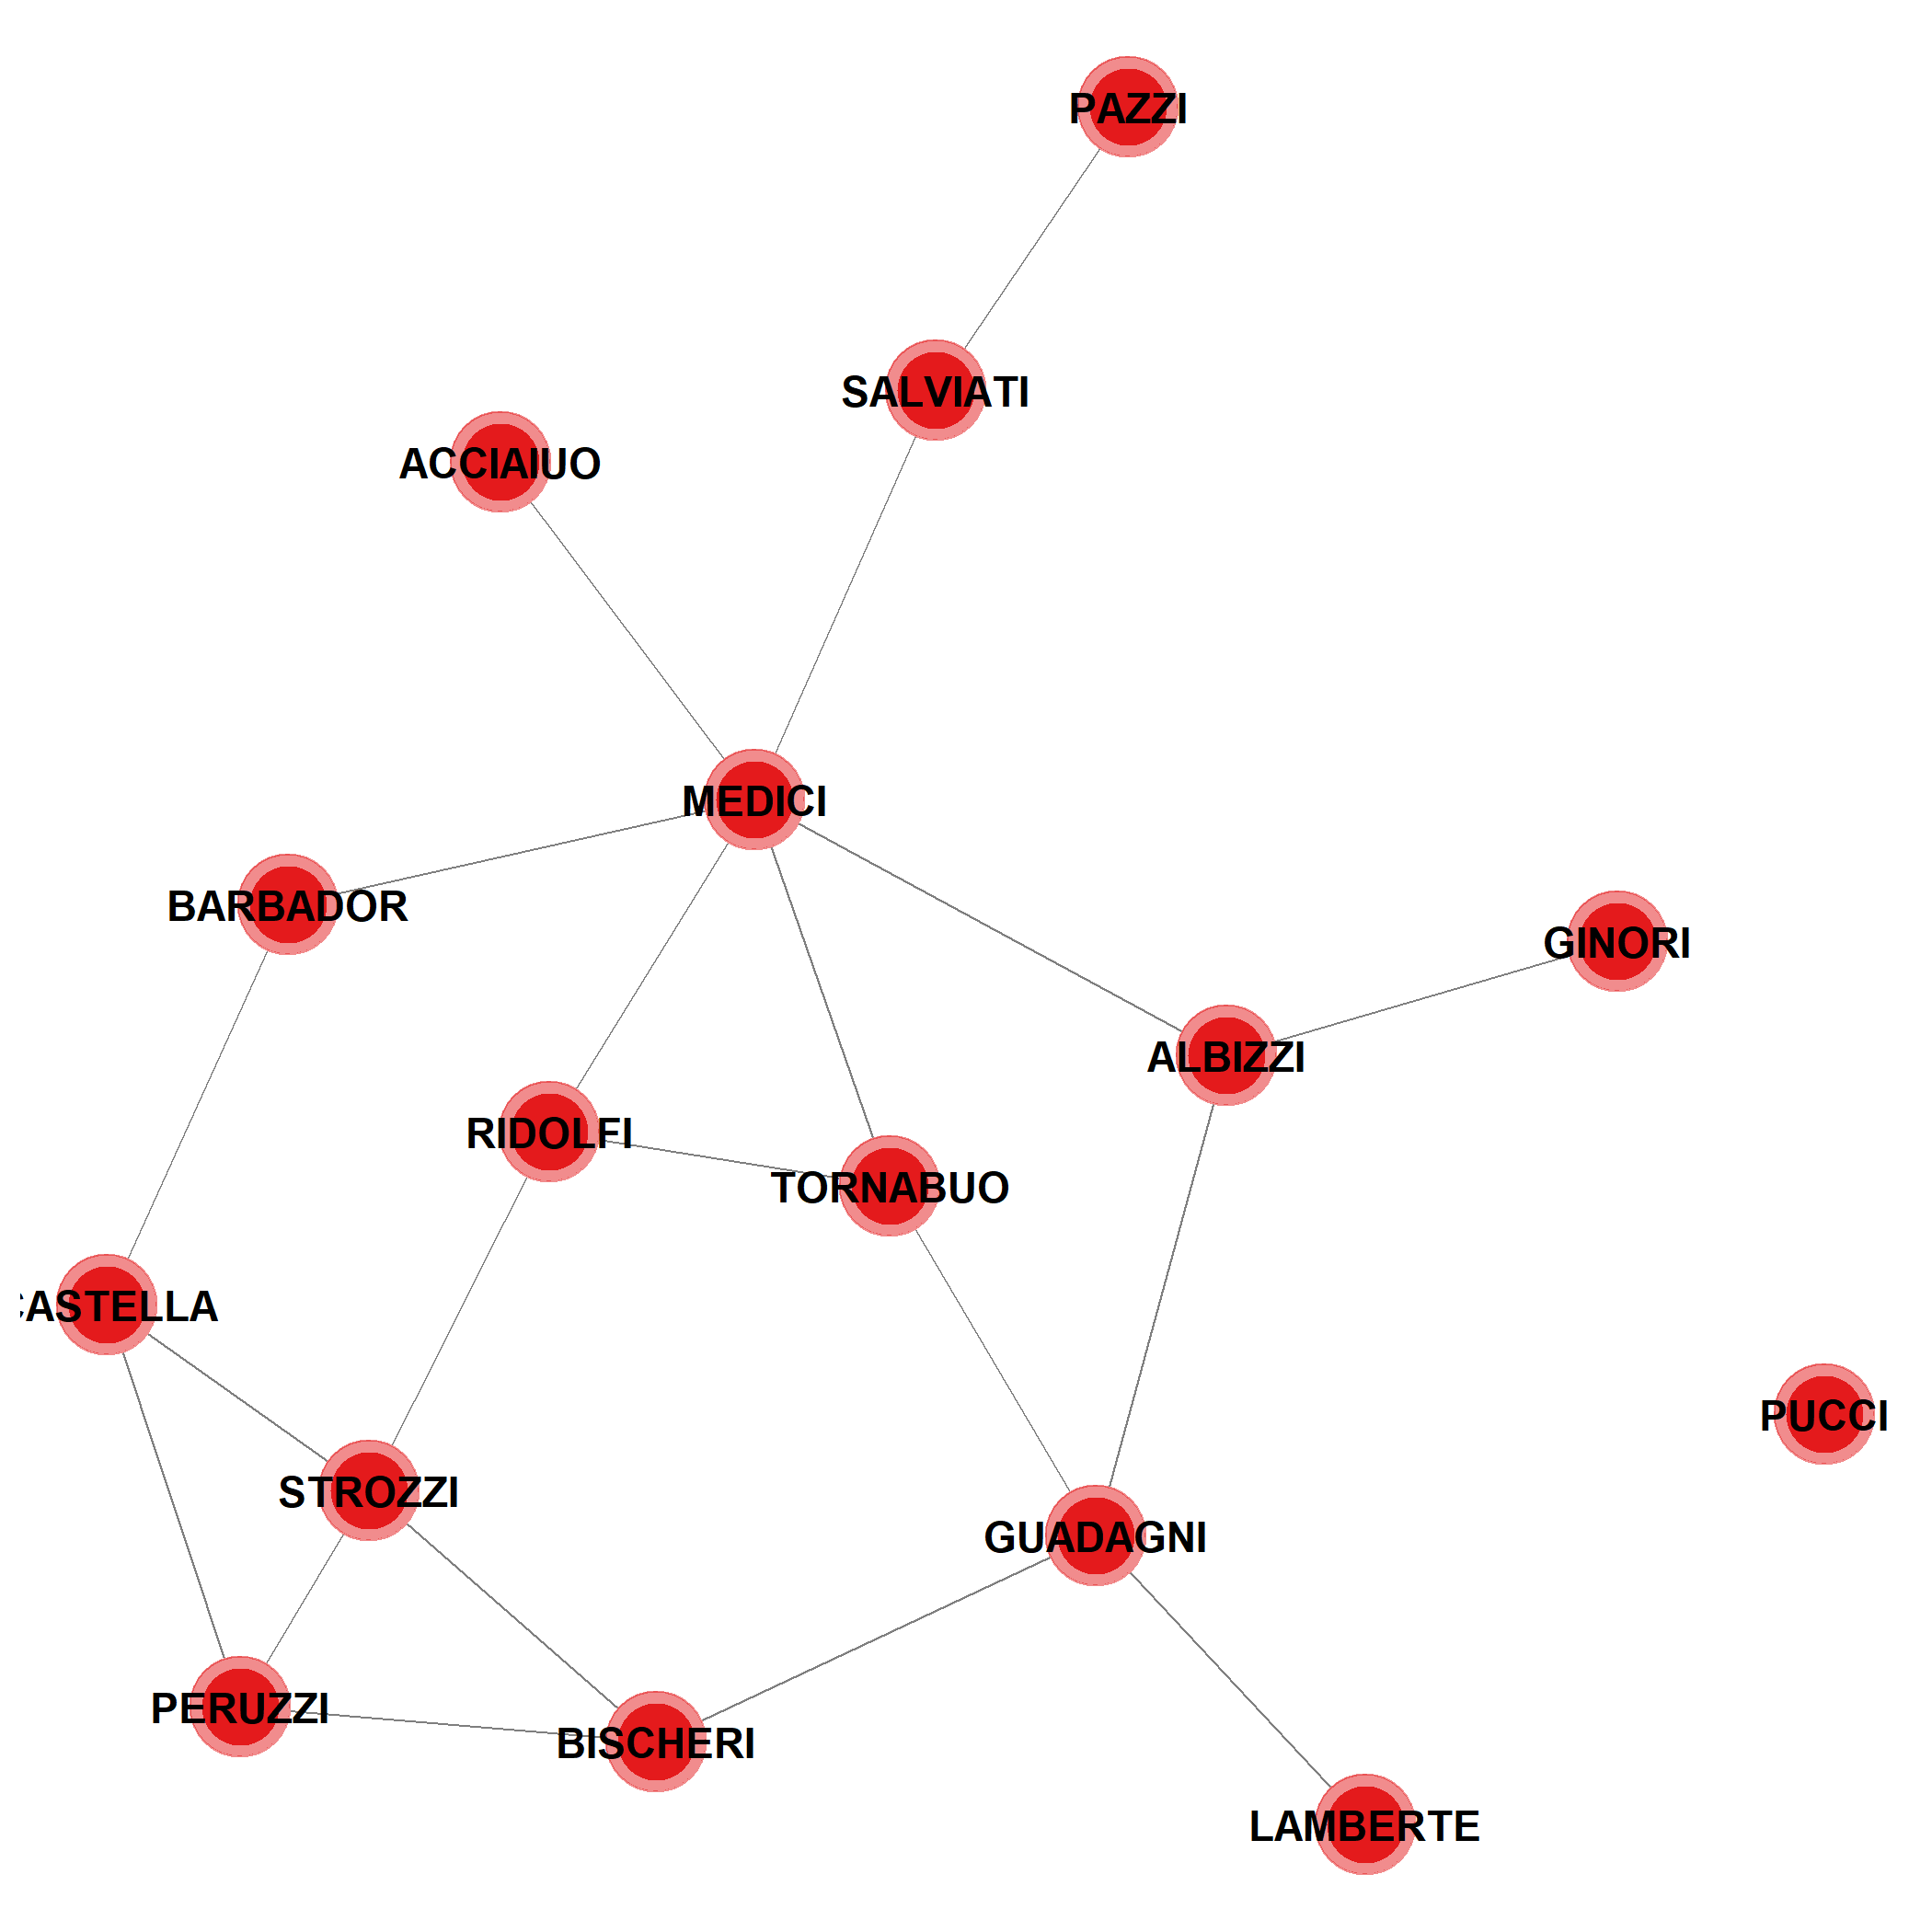
\includegraphics[width=.75\textwidth]{Tesis/Figures/Florentine.png}
\caption{El Matrimonio Florentino}
\centering
\end{figure}

Empezamos con el modelo de tal forma que expresemos nuestro modelo.

\begin{equation*}
    \textit{Florentino} \sim \textit{Numero.de.Aristas}
\end{equation*}

\begin{equation*}
    \log \left( \exp \left( \theta ^ { \prime } g ( y ) \right) \right) = \theta _ { 1 }  \sum _ { i , j > i \in \mathcal{N} } y _ { i j }.    
\end{equation*}

El modelo nos entrega entonces los estimadores de los parámetros de tal forma que nuestro estimador de $\theta_1=-1.6094$  y nos da un valor p significativo. ¿Cómo interpretamos esto?

\begin{equation*}
\begin{split}
    \operatorname{logit}(p(y))&=\theta \times \delta(g(y))\\
    &=-1.6094 \times \Delta Numero\hspace{} de\hspace{} aristas \\
    &=-1.6094 \times 1
\end{split}
\end{equation*}


Para cada arista, agregar cualquier arista a nuestro grafo siempre incrementa nuestro número de aristas por 1. La probabilidad correspondiente es obtenida sacando el $logit$ inverso de $\theta$:

\begin{equation*}
\begin{split}
    &= \exp (-1.61) /(1+\exp (-1.61))\\
    &= 0.1665886
\end{split}
\end{equation*}

Interpretamos el modelo de tal forma que esta probabilidad corresponde a la densidad que observamos en nuestro grafo de $20$ aristas y un posible de $120$ aristas que pudiese haber con los 16 nodos. Es decir que la probabilidad de una arista es $20/120=.16\bar{6}$.

Avanzamos en nuestro proceso de modelaje añadiendo el término de triángulos para considerar un elemento de conglomerado:

\begin{equation*}
    \textit{Florentino} \sim \textit{Numero.de.Aristas} + \textit{Numero.de.Triángulos}
\end{equation*}

\begin{equation*}
    \log \left( \exp \left( \theta ^ { \prime } g ( y ) \right) \right) = \theta _ { 1 } \times \sum _ { i , j > i \in \mathcal{N} } y _ { i j }  + \theta_2    \times \sum _ { i j k }  y _ { i j } y _ { j k } y _ { k i } 
\end{equation*}

Este modelo nos brinda entonces que los valores estimados de los parámetros de las aristas son $\theta_1 = -1.6694$ y $\theta_2 = 0.1539$. Es decir que las log-\textit{odds} para que una arista no termine por crear ningún triángulo el condicional log-\textit{odds} es entonces de $-1.67$. Para que entonces forme un triángulo los log-\textit{odds} se convierte en $-1.67+ .0.1539 = -1.516$, entonces que se hagan dos triángulos tenemos que $-1.67+2 \times 0.1539 = -1.34$. Las correspondientes probabilidades entonces son $0.1584, 0.1801, 0.2039$ respectivamente.

Para este caso normalmente se puede utilizar el atributo de riqueza de cada familia con la covarianza entre cada familia como parte de nuestro modelo. Sin embargo, nos vamos a enfocar en las dinámicas orientadas a aristas ya que es lo que haremos más adelante. Además, también veremos el caso de los pesos geométricos con k estrellas y su correspondiente análisis.

Inspeccionado la última ronda de simulación antes del cálculo de las las estimaciones del parámetro tenemos acceso a la traza y la densidad de cada estadística.

\begin{figure}[t]
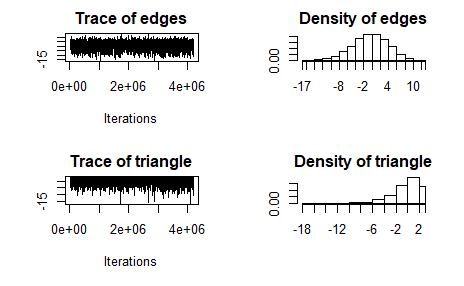
\includegraphics[width=1\textwidth]{Tesis/Figures/mcmcflorentine.jpg}
\caption{Diagnóstico de las cadenas de Markov}
\centering
\end{figure}

De aquí podemos observar que nuestro modelo se comporta de forma adecuada pues nuestras distribuciones están centradas y la traza es aleatoria. Aún así esto no nos garantiza que estos procesos locales estén capturando toda la información y que sean capaces de generar grafos que tengan las mismas propiedades globales.

Entonces simulamos 100 grafos con los parámetros estimados y comparamos en la siguiente tabla:

\begin{center}
 \begin{tabular}{||c c c||} 
 \hline
 Num & Aristas & Triángulo \\ [.5ex] 
 \hline\hline
 Obs & 20.00 & 3.0 \\ 
 \hline
 Media Simulada & 20.47 & 3.3  \\
 \hline
\end{tabular}
\end{center}

Vemos que nuestra estimación se encuentra bien ajustada para las aristas y que tiene un error del 10\% en esta serie de simulaciones.

\begin{figure}[h]
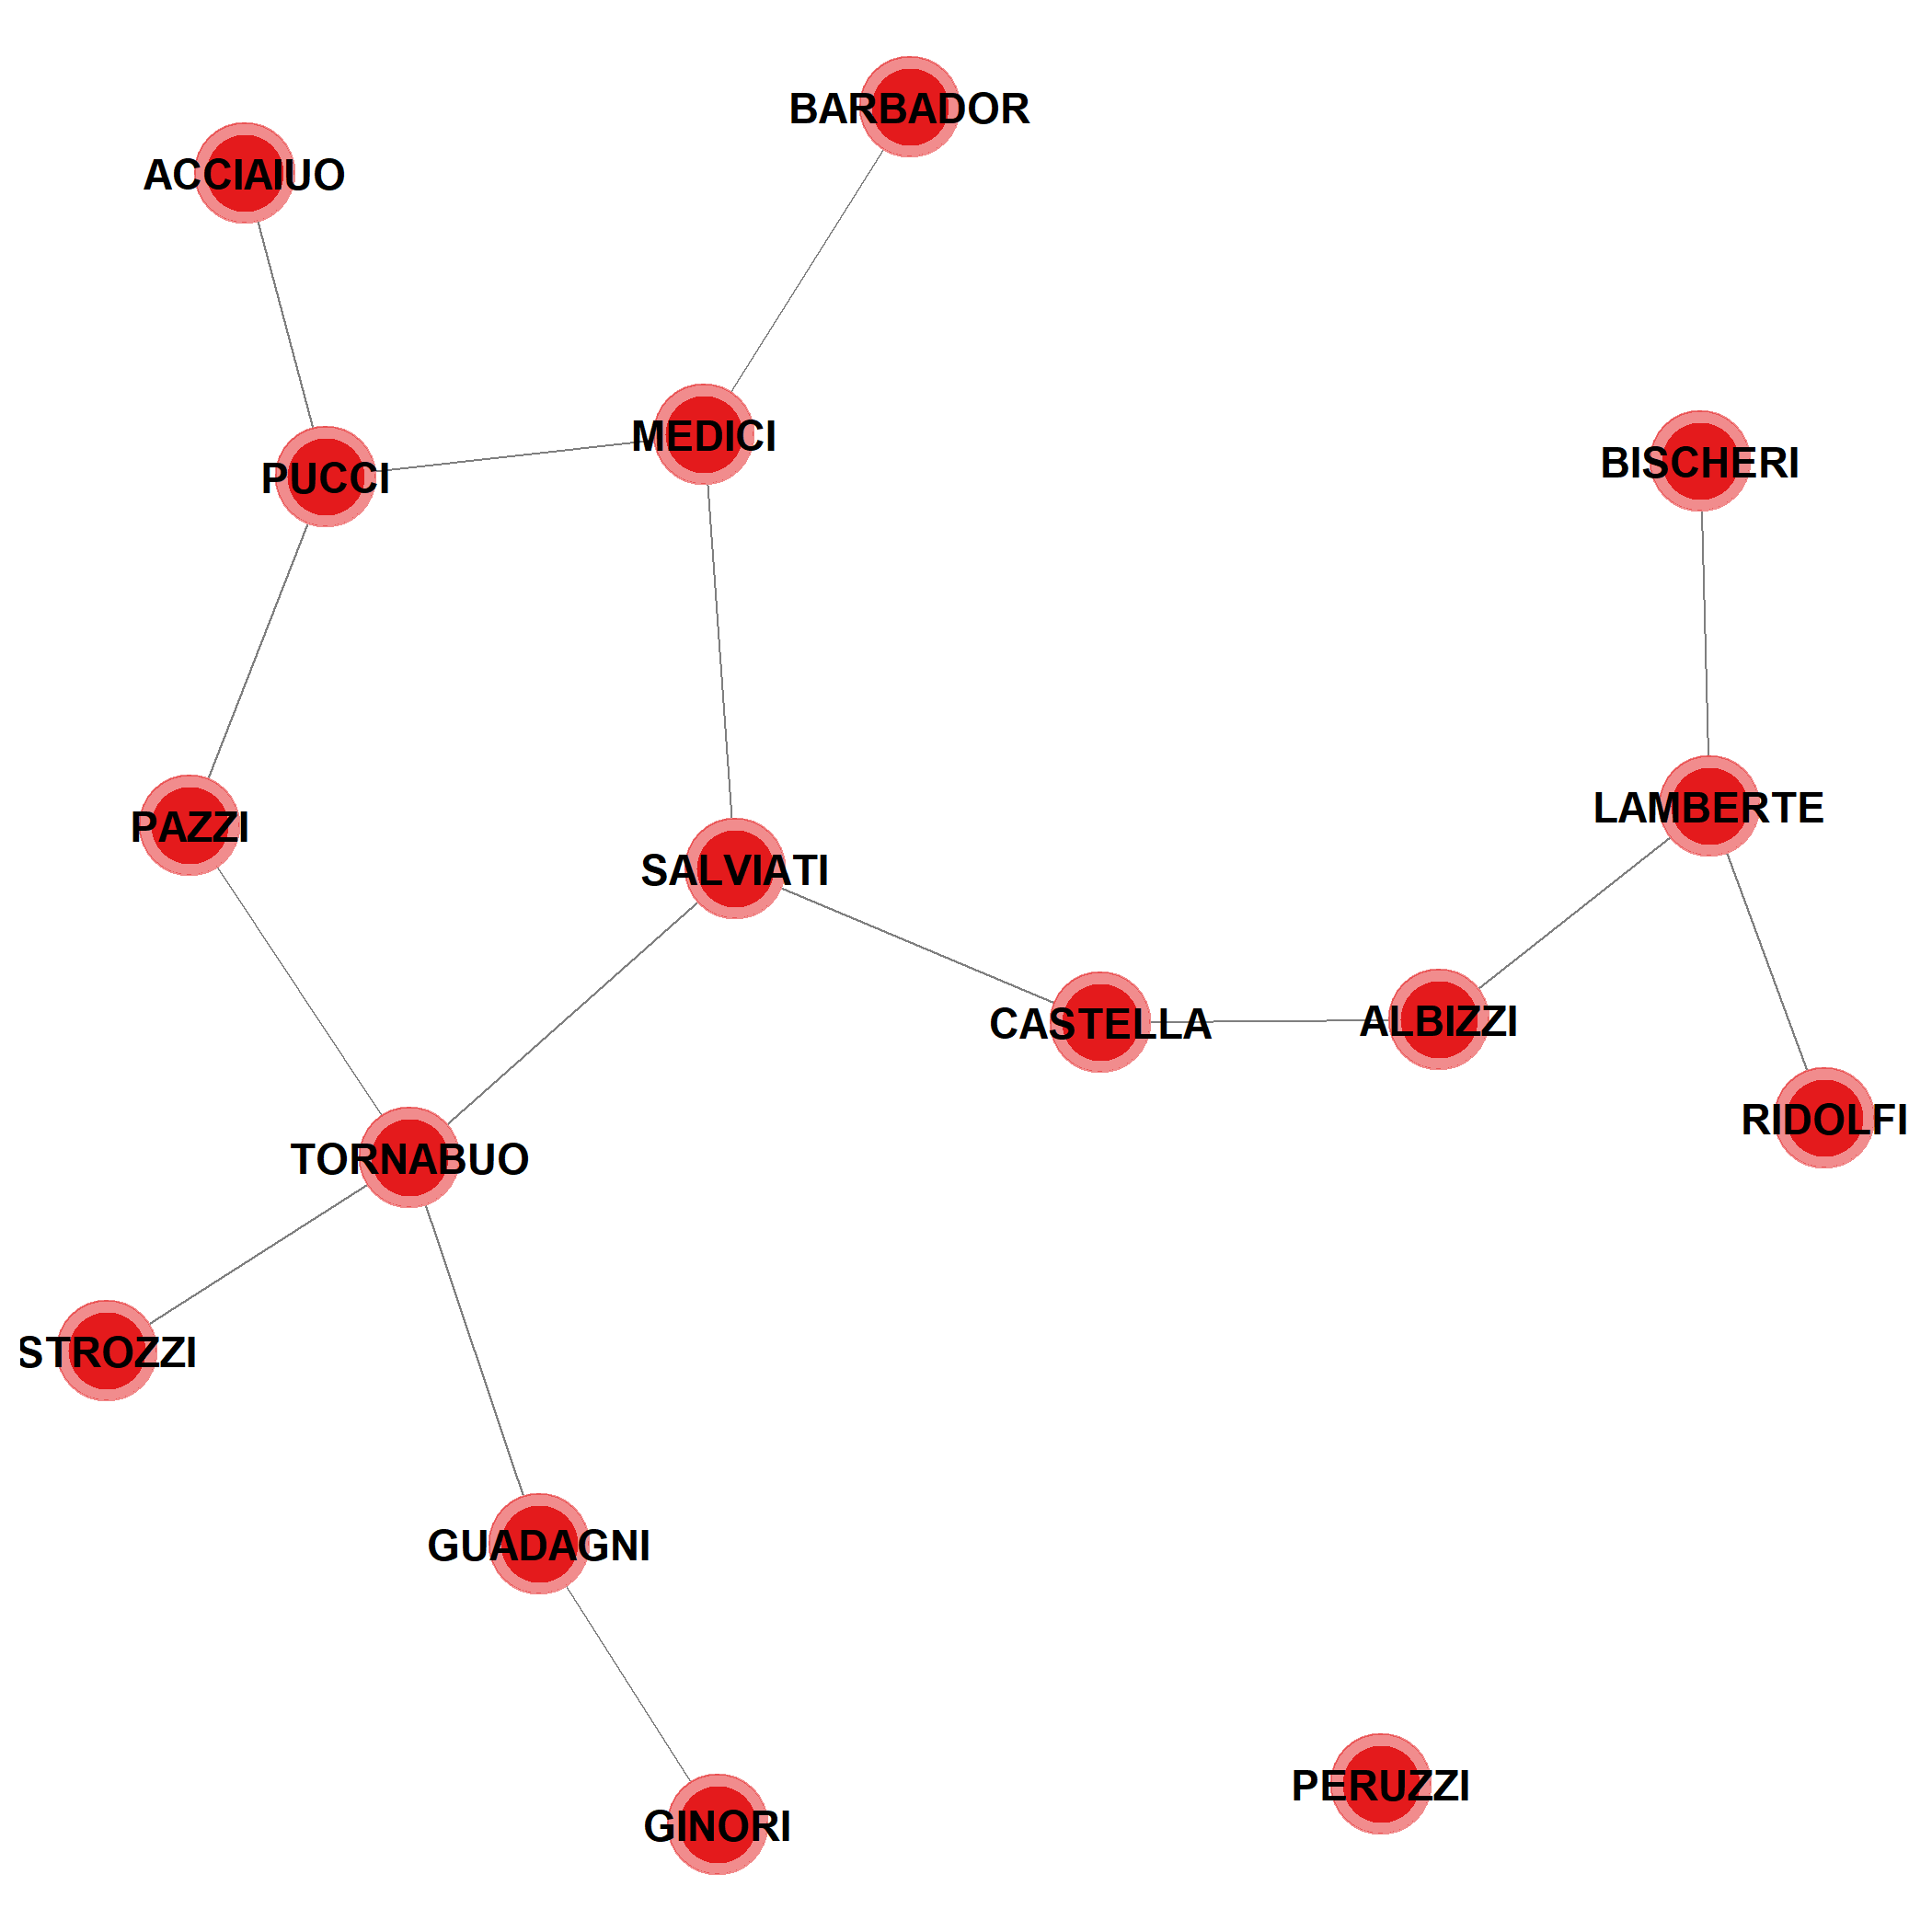
\includegraphics[width=.75\textwidth]{Tesis/Figures/FlorentineSIM.png}
\caption{Simulación de Matrimonio Florentino}
\centering
\end{figure}

También utilizamos las medidas de bondad de ajuste para ver qué tan buena es nuestra estimación. Con esto obtenemos la siguiente tabla de las medidas de bondad de ajuste y las correspondientes gráficas.

\begin{center}
 \begin{tabular}{||c c c c c c||} 
 \hline
 Estadística & obs & min & media & max & Valor p MC \\ [.5ex]
 \hline\hline
 Aristas & 20.00 & 9 & 19.30 & 29 & 1 \\ 
 \hline
 Triángulo & 3 & 0 & 2.67 & 10 & 1 \\
 \hline
\end{tabular}
\end{center}

\begin{figure}[h]
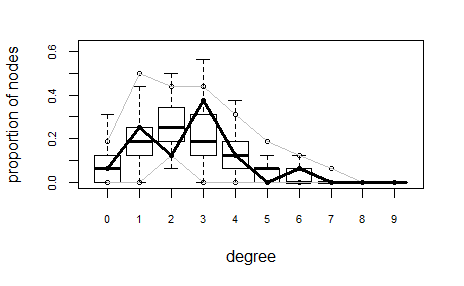
\includegraphics[width=.5\textwidth]{Tesis/Figures/Flo1mc.jpg}
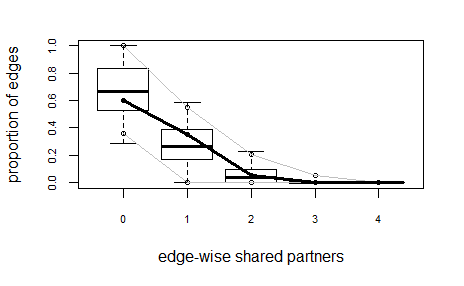
\includegraphics[width=.5\textwidth]{Tesis/Figures/flo2mc.jpg}
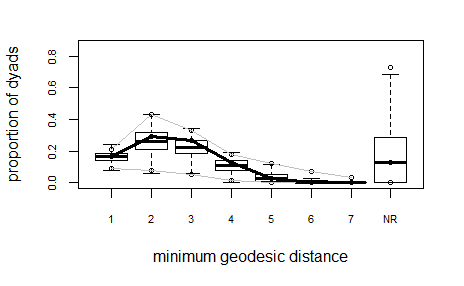
\includegraphics[width=.5\textwidth]{Tesis/Figures/flo3mc.jpg}
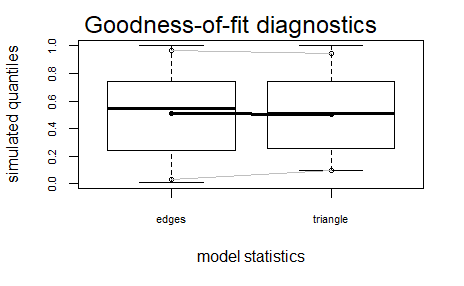
\includegraphics[width=.5\textwidth]{Tesis/Figures/flo4mc.jpg}
\caption{Medidas de Bondad con triángulo}
\centering
\end{figure}

Así que seguimos iterando e implementamos un modelo con otra útil medida de Asociaciones compartidas perimetrales ponderadas geométricamente cuyas estadísticas de descritas por \cite{hunter2007curved} son


\begin{*equation}

\delta w = e^{\alpha}\{1-(1-e^{-\alpha})^1\} \times 3 - e^\alpha{\{1-(1-e^{-\alpha})^0\}} \times 2

\end{*equation}

donde $\alpha$ es el parámetro de la medida de asociaciones compartidas perimetrales ponderadas geométricamente.

Remplazamos la estadística de triángulos por ésta y generamos nuestro modelo. Obtenemos que $\theta_1 = -1.709$ y que $\theta_2 = .1047$ con los siguientes diagnósticos. 

\begin{figure}[h]
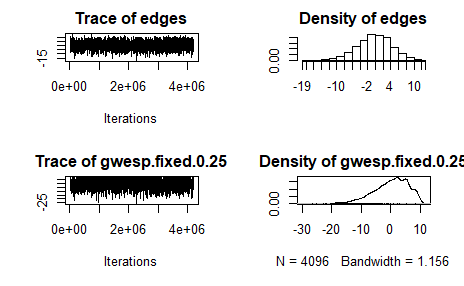
\includegraphics[width=1\textwidth]{Tesis/Figures/mcmcgwesp.jpg}
\caption{Diagnostico MCMC con medida geométrica.}
\centering
\end{figure}

Vemos que éste se ajusta mejor que con los triángulos pero es muy parecido. Con la comparación de las medidas de ajuste y sus correspondientes gráficas de bondad de ajuste en la Figura 5.6 entonces vemos que se ajustan de forma parecida y comparable.

\begin{center}
 \begin{tabular}{||c c c c c c||} 
 \hline
 Estadística & obs & min & media & max & Valor p MC \\ [.5ex]
 \hline\hline
 Aristas & 20.00 & 10 & 19.85 & 34 & 1 \\ 
 \hline
 Gwesp(.25) & 8.221 & 0 & 8.27 & 27.541 & .86 \\
 \hline
\end{tabular}
\end{center}



\begin{figure}[h]
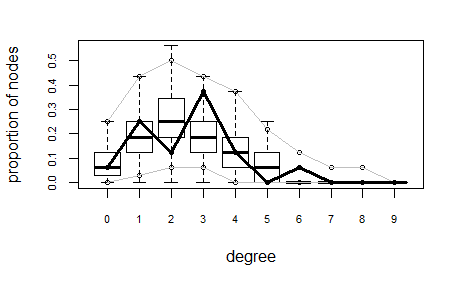
\includegraphics[width=.5\textwidth]{Tesis/Figures/gwespgof1.jpg}
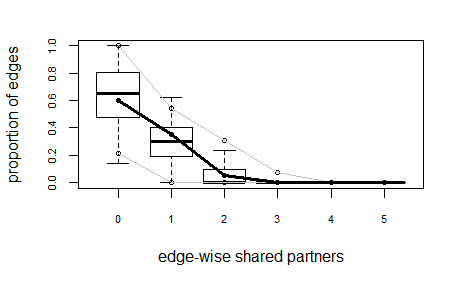
\includegraphics[width=.5\textwidth]{Tesis/Figures/gwespgof2.jpg}
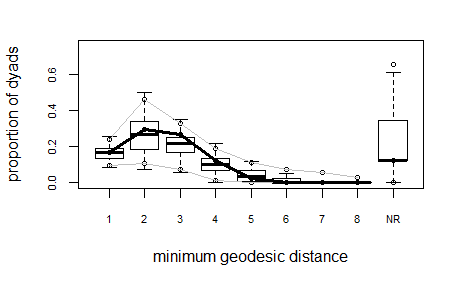
\includegraphics[width=.5\textwidth]{Tesis/Figures/gwespgof3.jpg}
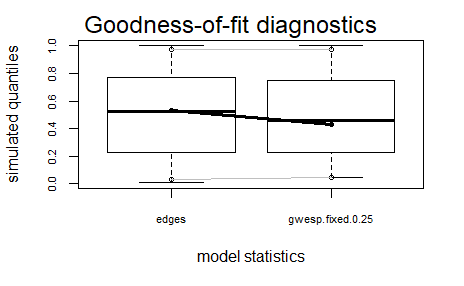
\includegraphics[width=.5\textwidth]{Tesis/Figures/gwespgof4.jpg}
\caption{Medidas de Bondad con GWESP(.25)}
\centering
\end{figure}



\section{Caso de navegación en internet}

Gracias a la generosa ayuda de la empresa Hexagon Data es que tenemos acceso a \textit{Lotame Data Stream} que es un servicio que proporciona acceso en tiempo real a datos de comportamiento sin procesar de cientos de millones de perfiles de navegadores de internet en millones de sitios web. Cada uno de estos registros de millones de \textit{cookies} vienen con información sobre cuándo es que se hicieron una serie de acciones en internet, el país en donde se hicieron, y el sitio web en donde se hicieron. Estos comportamientos entonces están catalogados por Lotame y sus clientes en una taxonomía maestra (ver anexo). Los datos representan el 1\% de todo el tráfico de usuarios de internet en Estados Unidos a través de varias semanas y suman alrededor de 9 millones de usuarios y 1,000 millones de comportamientos registrados. Sin embargo, no todos los comportamientos están catalogados, ya que sólo alrededor del 30$\%$ de la muestra está catalogada dentro de la taxonomía maestra. 

Un registro de una \textit{cookie} cualquiera se ve de la siguiente forma:
\begin{verbatim}
    {"id":{"val":"3c020b70ddec74ed22f6e6e676d2a952",
    "type":"cookie"},
    "country":"US","region":"na",
    "events":[{"tap":"DEVICE","src":"ldxsample1",
    "subSrc":"b590776e","ts":1537056014,
    "add":[8852078,34922299,2296544,41536150,52229337,
           648377,24729307],
    "remove":[33064974,41668881,41668880]}]}
\end{verbatim}

Es decir que este registro viene atado a una \textit{cookie} con id 3c020b70ddec74ed22f6e6e676d2a952 de Estados Unidos con región desconocida. Llevo a cabo su comportamiento en el momento 1537056014 en el sitio web b590776e y fueron 7 interacciones con el sitio web en ese momento. Adicionalmente también se le quitaron 3 comportamientos de forma programada pues no ha repetido esos comportamientos en los últimos 90 días. Sabemos entonces que esta lista de comportamientos están relacionadas a través del usuario. Sin embargo, no queremos relacionar estos identificadores de comportamiento unos con los otros pues son demasiado granulares y son únicos a los sitios web en donde viven. Entonces es que antes de generar una relación entre estos comportamientos es de conveniencia abstraer su significado a los elementos de la taxonomía del mercado de terceros en donde se compra y vende la información de estos usuarios.

Dos registros de la taxonomía del mercado de terceros se ven de la siguiente forma:

\begin{verbatim}
    {"behavior_id":41536150,"hierarchy_nodes
    ":[{"id":52650,
    "path":"Lotame Category Hierarchy^
    Sports & Recreation^Motorsports"}]}
    {"behavior_id":24729307,"hierarchy_nodes"
    :[{"id":525099,
    "path":"Lotame Data Selling Network - Location Hierarchy^
    Countries^North America^United States^Kansas"}]}
\end{verbatim}

Es decir que para el primer registro del \textit{behavior} está asignado al nodo de la taxonomía del mercado de terceros con id 52650  que corresponde al nodo \textit{Lotame Category Hierarchy\textasciicircum Sports & Recreation\textasciicircum Motorsports}. Haciendo este mismo análisis para el segundo registro y comparando con nuestro usuario vemos que nuestro usuario cualquiera está interesado en estos dos comportamientos a la vez. Entonces para la creación de nuestro grafo podemos garantizar que hay al menos una arista entre los nodos de Kansas y de \textit{Motorsports}. 

Así pues en términos matemáticos podemos representar esta relación como  un grafo bipartito en donde se tiene a los nodos de los usuarios de un lado conectados a los distintos nodos categoría de la taxonomía del otro lado. A través de esta representación es que podemos generar un grafo no dirigido en donde las categorías están conectadas entre sí a través del número de usuarios que tienen ambas categorías en su lista de comportamientos clasificados.

\begin{minipage}{1\linewidth}
\begin{figure}[H]\centering

\begin{tikzpicture}[ scale=1.2]
\tikzset{vertex/.style = {shape=circle,draw,minimum size=2.2em}}
\tikzset{edge/.style = {->,> = latex}}


\filldraw[color=green!60, fill=green!5, very thick](0,-.5) ellipse (1.2 and 6);
\filldraw[color=red!60, fill=red!5, very thick](4,0) ellipse (1 and 5);
\filldraw[color=blue!60, fill=blue!5, very thick](8,0) ellipse (.8 and 5);


% vertices
% 
\node[vertex] (a) at (4,3) {$B_1$};
\node[vertex] (b) at (4,2) {$B_2$};
\node[vertex] (c) at (4,1) {$B_3$};
\node[vertex] (d) at (4,0) {$B_4$};
\node[vertex] (e) at (4,-1) {$B_5$};
\node[vertex] (e1) at (4,-2) {$B_6$};
\node[vertex] (e2) at (4,-3) {$B_7$};
\node[vertex] (e3) at (4,-4) {$B_8$};


\node[vertex] (g) at (0,4) {$C_1$};
\node[vertex] (h) at (0,3) {$C_2$};
\node[vertex] (i) at (0,2) {$C_3$};
\node[vertex] (j) at (0,1) {$C_4$};
\node[vertex] (k) at (0,0) {$C_5$};
\node[vertex] (l) at (0,-1) {$C_6$};
\node[vertex] (m) at (0,-2) {$C_7$};
\node[vertex] (n) at (0,-3) {$C_8$};
\node[vertex] (o) at (0,-4) {$C_9$};
\node[vertex] (p) at (0,-5) {$C_{10}$};


\node[vertex] (g1) at (8,4) {$T_1$};
\node[vertex] (h1) at (8,3) {$T_2$};
\node[vertex] (i1) at (8,2) {$T_3$};
\node[vertex] (j1) at (8,1) {$T_4$};
\node[vertex] (k1) at (8,0) {$T_5$};
\node[vertex] (l1) at (8,-1) {$T_6$};
\node[vertex] (m1) at (8,-2) {$T_7$};
\node[vertex] (n1) at (8,-3) {$T_8$};
\node[vertex] (o1) at (8,-4) {$T_9$};


\node (w) at (0,6) {Cookies};
\node (x) at (4,6) {\textit{Behavior}};
\node (x) at (8,6) {Taxonomía};


\path[-stealth] (g) edge (a);
\path[-stealth] (g) edge (b);
\path[-stealth] (g) edge (c);
\path[-stealth] (g) edge (d);
\path[-stealth] (h) edge (a);
\path[-stealth] (i) edge (b);
\path[-stealth] (j) edge (b);
\path[-stealth] (k) edge (e);
\path[-stealth] (k) edge (e1);
\path[-stealth] (k) edge (e2);
\path[-stealth] (k) edge (e3);
\path[-stealth] (l) edge (c);
\path[-stealth] (m) edge (d);
\path[-stealth] (n) edge (b);
\path[-stealth] (o) edge (d);
\path[-stealth] (p) edge (d);
%\path[-stealth] (b) edge (g);


\path[-stealth] (a) edge (g1);
\path[-stealth] (b) edge (h1);
\path[-stealth] (b) edge (i1);
\path[-stealth] (c) edge (j1);
\path[-stealth] (d) edge (k1);
\path[-stealth] (e) edge (l1);
\path[-stealth] (e1) edge (l1);
\path[-stealth] (e2) edge (m1);
\path[-stealth] (e3) edge (n1);

%\draw (4,4) node[cross=8pt,red] {};


%\draw (0.2,8)--(3.8,8);



\end{tikzpicture}
\caption{ Representación de las relaciones }
\end{figure}
\end{minipage}


Vale la pena notar la relación entre \textit{behavior} y los nodos de la taxonomía puede ser de uno a muchos. Darle clic a un artículo cuyo título es \textbf{presidente propone la cancelación de los puentes} puede tener asociado los temas de Política, Turismo y México. En la Figura 5.1 podemos observar que $T_6$ y $T_7$ y $T_{8}$  están relacionados a través de $C_5$. Al igual que $T_1, T_2, T_3,T_4$ y $T_5$ están relacionados a través de $C_1$


Sin embargo, la taxonomía tiene más de 5000 nodos categoría cuando la tomamos en su forma original. Sin embargo dada la estructura jerárquica de la taxonomía es que podemos ""subirla de nivel"" para reducir el número de nodos. Por ejemplo, podríamos en vez de tomar el nodo en la taxonomía de \textit{Lotame - Media & Entertainment - Sports - Team Sports - Football Soccer - International Competiton} podemos decidir catalogarlo simplemente como \textit{Lotame - Media & Entertainment - Sports - Team Sports - Football Soccer}. Sin embargo, perdemos cierto nivel de granularidad. Para esta tesis se hizo un desglose artesanal de cada tipo de comportamiento de acuerdo a su naturaleza para reducir el número de nodos categoría pero aún manteniendo una estructura general fiel al contenido de la taxonomía original.

Los modelos de grafos exponenciales tienen muchas formas y la cantidad de teoría detrás de cada tipo de modelaje como el ajuste del modelo a través del tiempo con grafos temporales o en este caso utilizando el grafo que es generado con los usuarios como nodos conectados por sus comportamientos durante un periodo en el tiempo. También sería posible crear un grafo en donde se usen los sitios web en donde sucedieron los comportamientos catalogados conectados con aristas basadas en el contenido, y así medir y predecir la cercanía en el contenido de distintos sitios web. 

\subsubsection{Nuestros Nodos Construidos}

Para simplificar nuestro caso restringimos el número de nodos de nuestro grafo para que estén limitados a intereses, \textit{hobbies} y medios. Es decir que los nodos que se refieren a información tecnográfica (con excepción del sistema operativo) y geográfica han sido eliminados para reducir de forma drástica la complejidad del problema y de esta forma de más de cinco mil nodos de la taxonomía es que tenemos un caso donde tenemos alrededor de 729 nodos de donde viene información más general. Sin embargo, el grafo generado con las categorías de estas taxonomías consiste de al menos dos subgrafos inducidos que no comparten ninguna arista entre ellos; en realidad hay muchos nodos totalmente desconectados. Por lo tanto el modelo de ERGMs solamente se corrió sobre el subgrafo máximo inducido de los presentes.


\subsection{Explorando las propiedades de nuestro grafo}


Nuestra muestra proviene del muestreo de la unidad de tiempo UNIX 1536267600 equivalente a 06/09/2018 a las 9:00 a.m. hasta tiempo UNIX 1537286399 equivalente a  18/09/2018 a las 3:59 p.m. de donde la matriz de adyacencia que fue obtenida del muestreo de combinaciones en dos. Se procesaron alrededor de 38.4762 GB de datos comprimidos de \textit{streaming} en el periodo mencionado o alrededor de 25,435,675 registros individuales con los cuales se hicieron las combinaciones. Los \textit{scripts} de Python utilizados para la extracción de la información de los  del \textit{stream} y el algoritmo para la creación de las aristas entre los nodos de contenido viene anexado de igual forma y entrega listas de aristas. El código de R para la manipulación de las tablas para convertir 
los datos a objetos de \textit{network} en R y para el modelaje de \textit{ERGMs} en \textit{statnet} también viene anexado. 

Desafortunadamente, el grafo generado de 729 nodos que está aquí ilustrado con colores del nodo que indican sus categorías en general se encuentra desconectado como ya fue mencionado. El grafo original contiene 111,131 aristas es decir que tiene una densidad de 0.209. 

\begin{figure}[!ht]
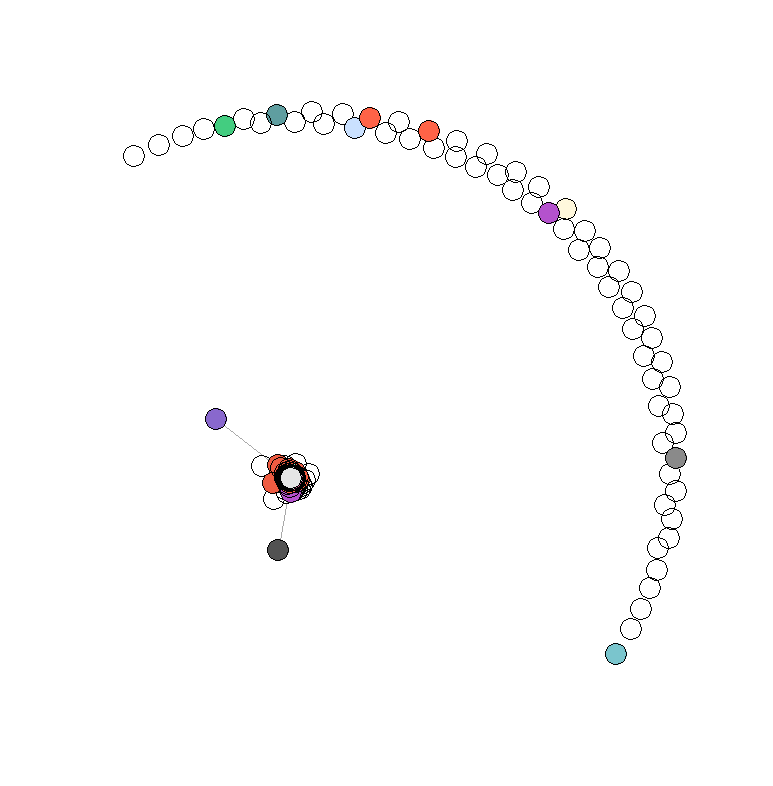
\includegraphics[width=1\textwidth]{Tesis/Figures/LotameFull.png}
\caption{Grafo de las cookies completo de Lotame con colores por tema.}
\centering
\end{figure}

Para el modelo en realidad vamos a elegir el subgrafo inducido y vamos a eliminar las aristas de peso del cuartil más chico para sólo quedarnos con las aristas que tienen mayor interacción, entonces eliminamos todas las aristas de peso menor a 46. El peso de cada arista se determinó a partir del número total de \textit{cookies} que tenían ambos comportamientos en sus eventos. La mediana del peso de las aristas entonces fue de 145 y el mayor peso reportado de 2,068,796 entre los nodos 52200 y 52413, que son el \textit{Lotame Category Hierarchy - Fashion & Beauty-Clothing} y \textit{Lotame Category Hierarchy - Health & Medicine - Physical Fitness} respectivamente. Una mejora posible en el muestreo sería diagnosticar cuáles usuarios en realidad son \textit{bots} que recorren una gran parte del contenido del grafo completo y eliminarlos del muestreo pero esto está fuera del alcance de esta tesis. A continuación se encuentra el histograma del log peso de las aristas en el grafo antes de hacer el filtro del cuartil más bajo y elegir el subgrafo inducido mas grande.

\begin{figure}[!ht]
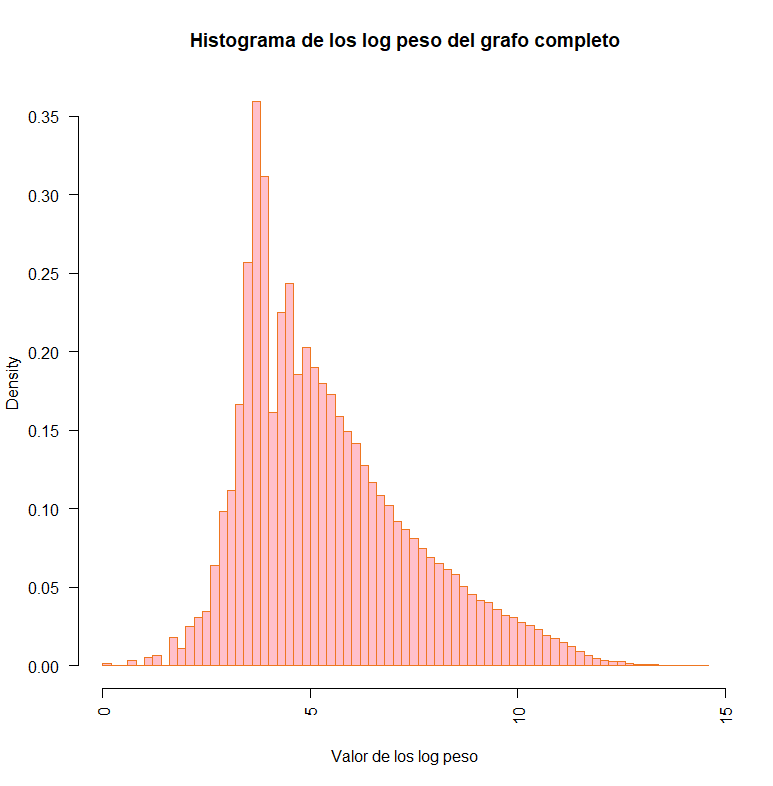
\includegraphics[width=1\textwidth]{Tesis/Figures/HistGrafoCompleto.png}
\caption{Histograma de $\log$ peso del grafo completo de las \textit{cookies} de Lotame.}
\centering
\end{figure}

Entonces nuestro grafo final cuenta con 662 nodos, cuyos elementos se encuentran anexados al final de esta tesis. Cuenta con 84580 aristas es decir que tiene una densidad de 0.193 y podemos dormir tranquilos que al menos esa estadística global es comparable a la de nuestro grafo original. Sin embargo el comportamiento de decadencia exponencial en los pesos de las aristas se ve mucho mejor con la muestra reducida.

\begin{figure}[!ht]
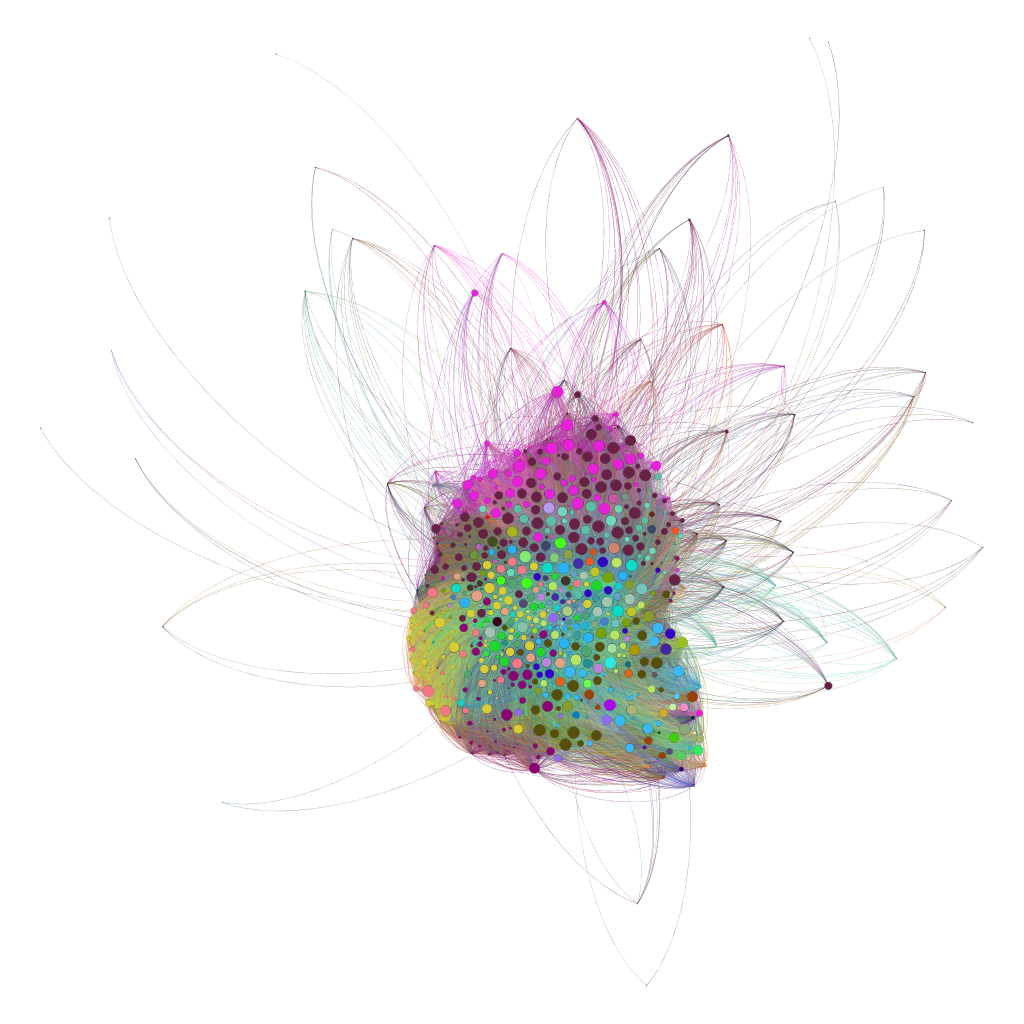
\includegraphics[width=1\textwidth]{Tesis/Figures/LotameFullgraphAmazing.png}
\caption{Subgrafo inducido de la muestra filtrada ordenado por categorías por color y ordenados principalmente con \textit{Force Atlas}.}
\centering
\end{figure}

\begin{figure}[!ht]
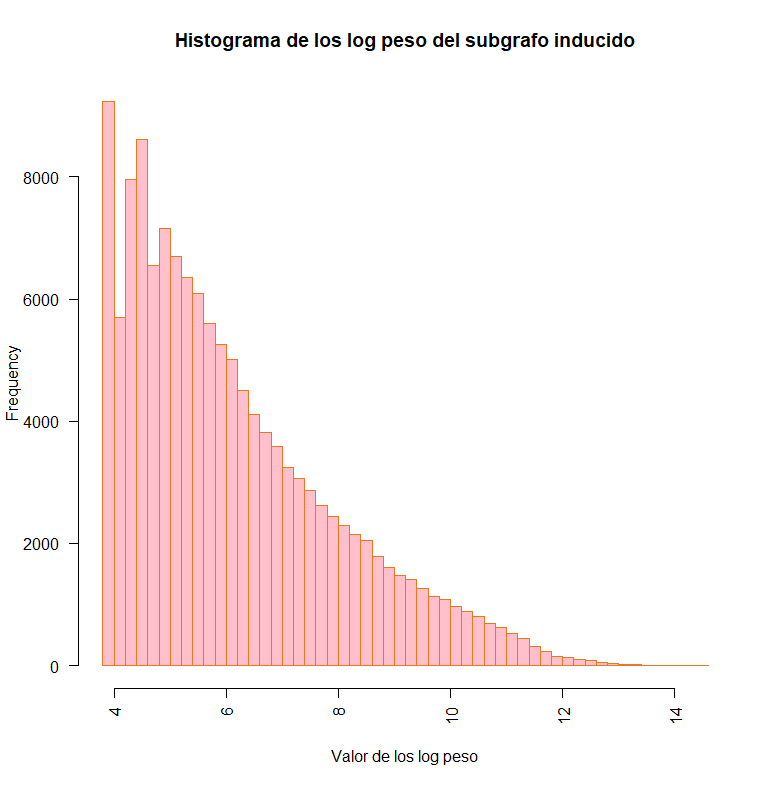
\includegraphics[width=1\textwidth]{Tesis/Figures/HistSubgrafoInducido.png}
\caption{Histograma de $\log$ peso del subgrafo inducido de las cookies de Lotame.}
\centering
\end{figure}
\clearpage

\begin{figure}
 \begin{adjustwidth}{-3.6cm}{}
 \begin{tabular}{||C{2em} C{1em}||}
 \hline
 Nodo & Nodo \\ 
 \hline\hline
Computers and Technology-Operating \\
systems	&	Mobile  Wireless Devices-
Mobile Phones	\\
 \hline
 Fashion and \\
Beauty-Clothing	&	Health and Medicine-Physical Fitness	\\
 \hline
Home and Family-Lawn and \\
Garden	& Home and Family-Home Improvement	\\
\hline
Travel-Business Travel	& Physical Fitness	\\
\hline
Purchase Intent-Food, Beverages and \\
Tobacco-Food Items	&	Health and Medicine	\\
\hline
Purchase Intent-\\
Food, Beverages and Tobacco-\\
Food Items	&	Home and Family-
Lawn and Garden	\\
\hline
Purchase Intent-\\
Food, Beverages and Tobacco-\\
Food Items	&	Food and Beverages-
Recipes and Cooking	\\
\hline
Purchase Intent-\\
Food, Beverages and Tobacco-
Food Items	& Literature-Books	\\
\hline
Lawn and Garden	&	Home Improvement\\ [4ex] 

 \hline
\end{tabular}


 \end{adjustwidth}
 \caption{Los nodos con mayor número de conexiones por usuarios entre ellos.}
\end{figure}











\subsection{Propuesta de distintos modelos}

Aunque empezamos de la misma forma que en el caso florentino en donde tenemos que

\begin{equation*}
    \textit{Lotame} \sim \textit{Numero.de.Aristas}
\end{equation*}

\begin{equation*}
    \log \left( \exp \left( \theta ^ { \prime } g ( y ) \right) \right) = \theta _ { 1 }  \sum _ { i , j > i \in \mathcal{N} } y _ { i j }.    
\end{equation*}

El modelo Bernoulli fracasó y nos indica que esta estadística del grafo se encuentra en el máximo utilizando la estimación de la máxima pseudo verosimilitud.




\begin{equation*}
    \textit{Lotame} \sim  \textit{Numero.de.Triángulos+Numero.de.Aristas}
\end{equation*}

\begin{equation*}
    \log \left( \exp \left( \theta ^ { \prime } g ( y ) \right) \right) =  \theta_1    \times \sum _ { i j k }  y _ { i j } y _ { j k } y _ { k i } 
\end{equation*}



% \begin{equation*}
% \begin{split}
%     &= \exp (0.2325684) /(1+\exp (0.2325684 ))\\
%     &= 0.387
% \end{split}
% \end{equation*}

Después de un poco de exploración de datos y con los diagnósticos de Markov obtenidos para los valores de los parámetros de $\theta_1 = 0.02168062$ y $\theta_2 = -3.26154720$ sospechamos que necesitamos una mejor estadística que éstas para este grafo. Podemos observar los diagnósticos de las cadenas de Markov Monte Carlo en la figura 5.13 y no se ven muy bien. Detenemos el analisis de este modelo y proponemos el modelo con la medida de estrellas alternantes definida en \cite{Snidjers2006}.

\begin{figure}[!ht]
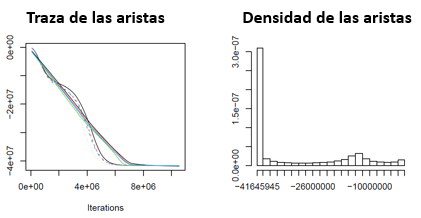
\includegraphics[width=1\textwidth]{Tesis/Figures/mcmc_1.PNG}
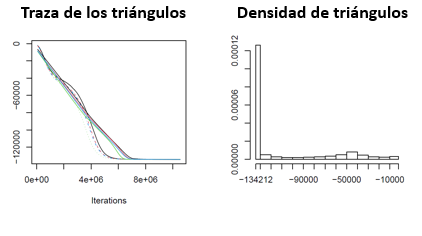
\includegraphics[width=1\textwidth]{Tesis/Figures/mcmc_2.PNG}

\caption{Diagnósticos de Markov del modelo de Triángulos y Aristas.}
\centering
\end{figure}

¡Eureka! Nuestro modelo converge en los valores de $\theta_1 = 16.5167$ y $\theta_2 = -15.2282$ y cuya constante de normalización es $\lambda = 0.5574$. Los diagnósticos de Monte Carlo de la Figura 5.13 se ven bien, pensando que la covariabilidad que se observa entre la traza de aristas y de estrellas alternantes es esperada por \cite{GoodOfFitSocialNetwork}, pues este modelo es equivalente al de los pesos geométricos por razones obvias. Parece que las medidas de bondad de ajuste también parecen ser capaces de ser relativamente buenas para imitar al menos algunos atributos globales de forma parecida a nuestro grafo original. Ver la figura 5.15 para inspeccionar las estadísticas de la bondad de ajuste.

\begin{figure}[!ht]
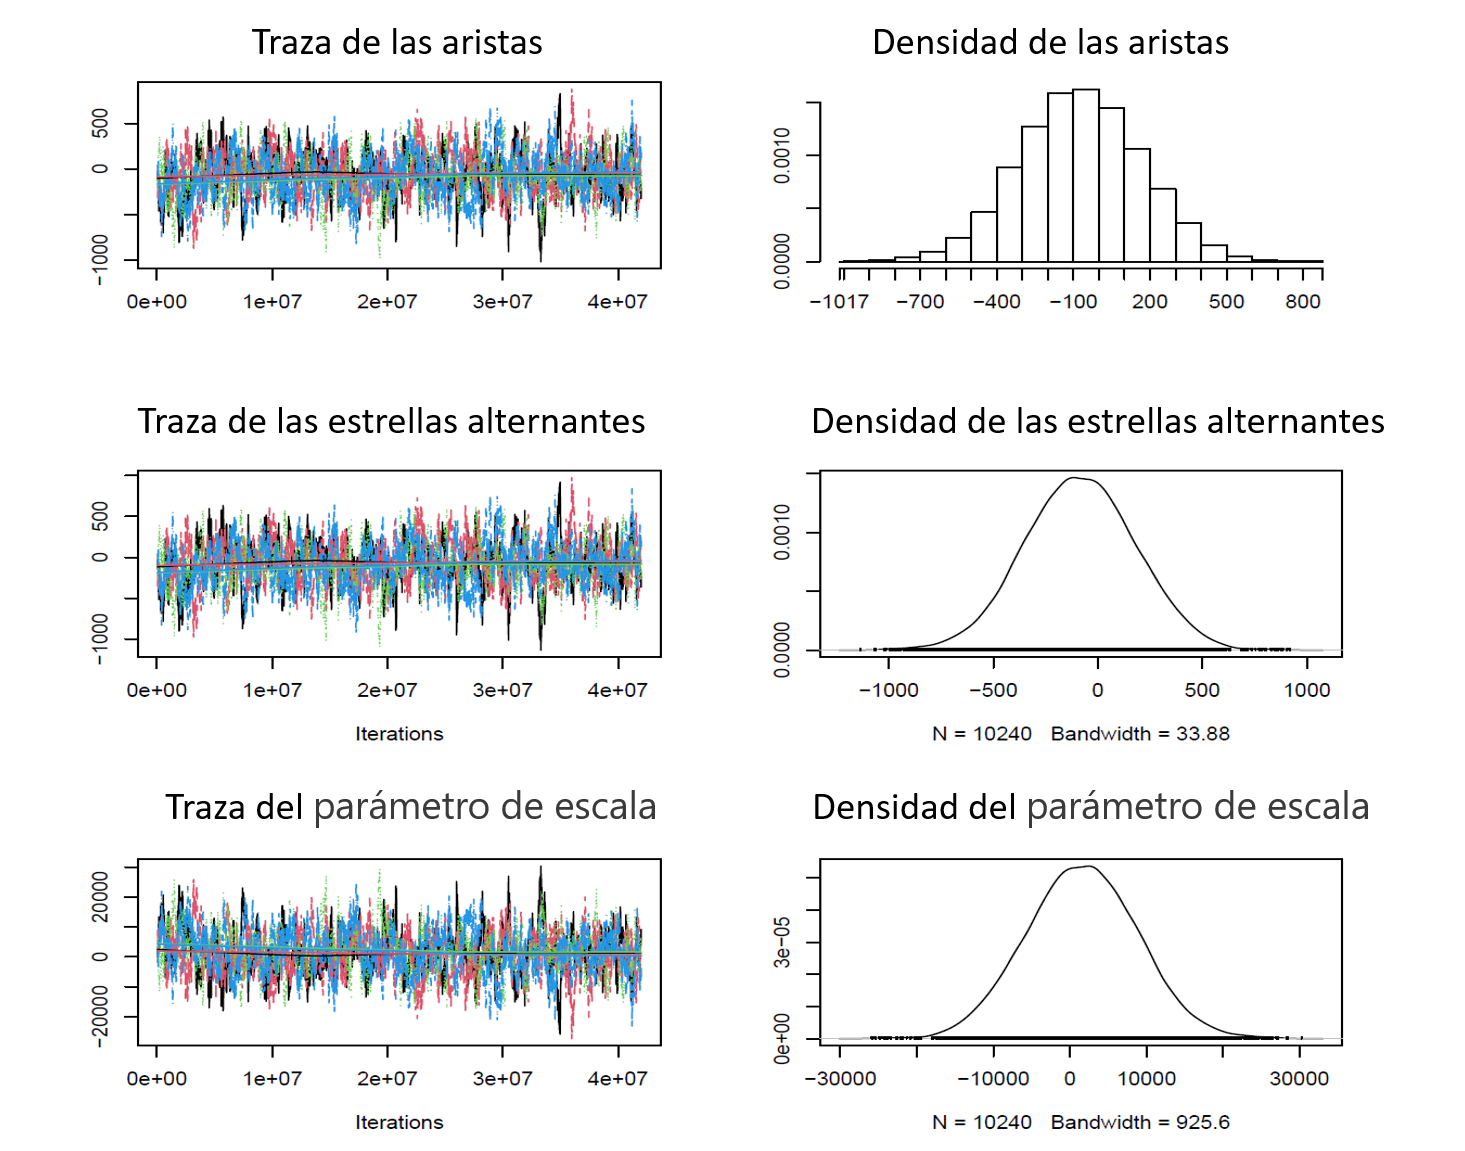
\includegraphics[width=1\textwidth]{Tesis/Figures/mcmc3.PNG}
\caption{Diagnósticos de Markov del modelo de Triángulos y Aristas.}
\end{figure}

\begin{figure}[!ht]
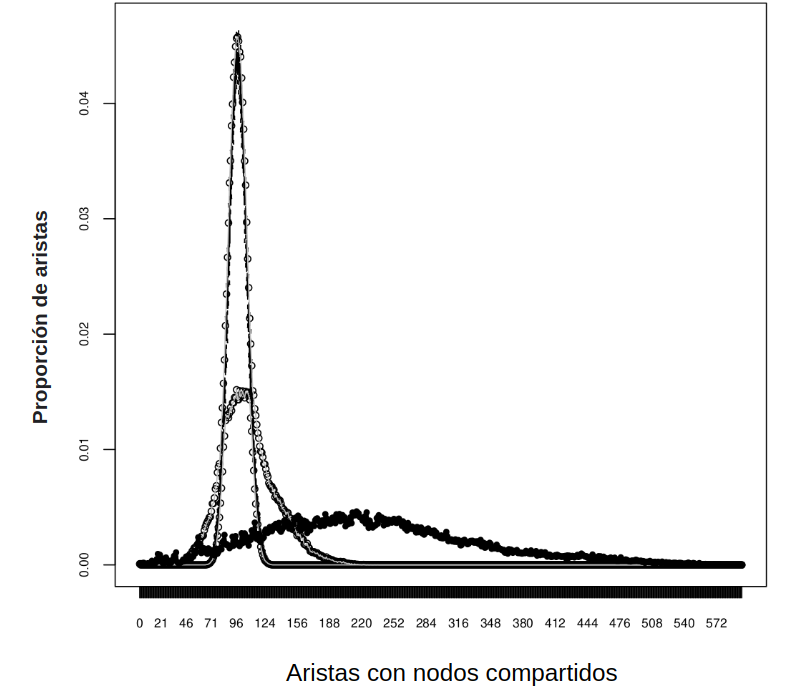
\includegraphics[width=.5\textwidth]{Tesis/Figures/gof_1_aristas_nodos_compartidos.png}
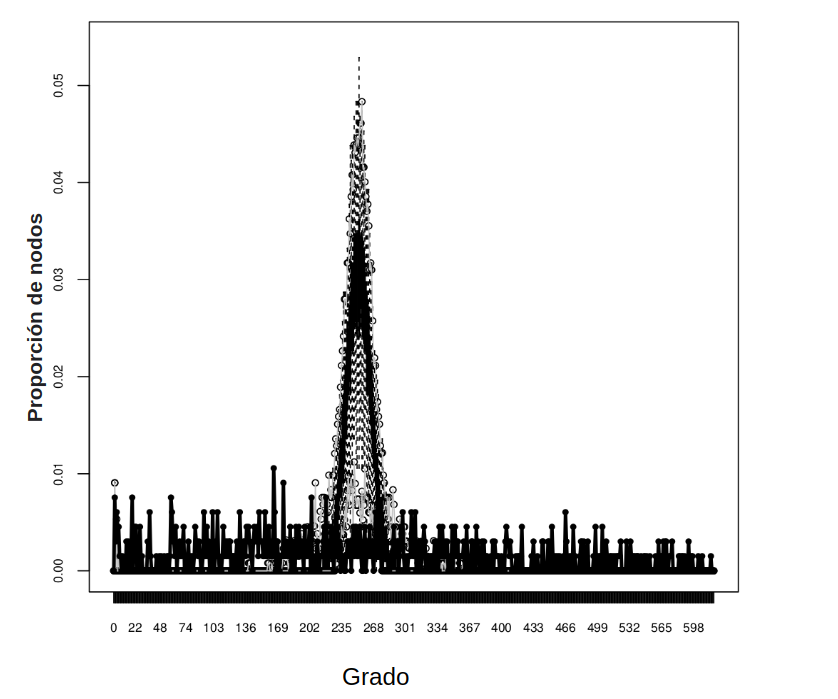
\includegraphics[width=.5\textwidth]{Tesis/Figures/gof_1_degree.png}
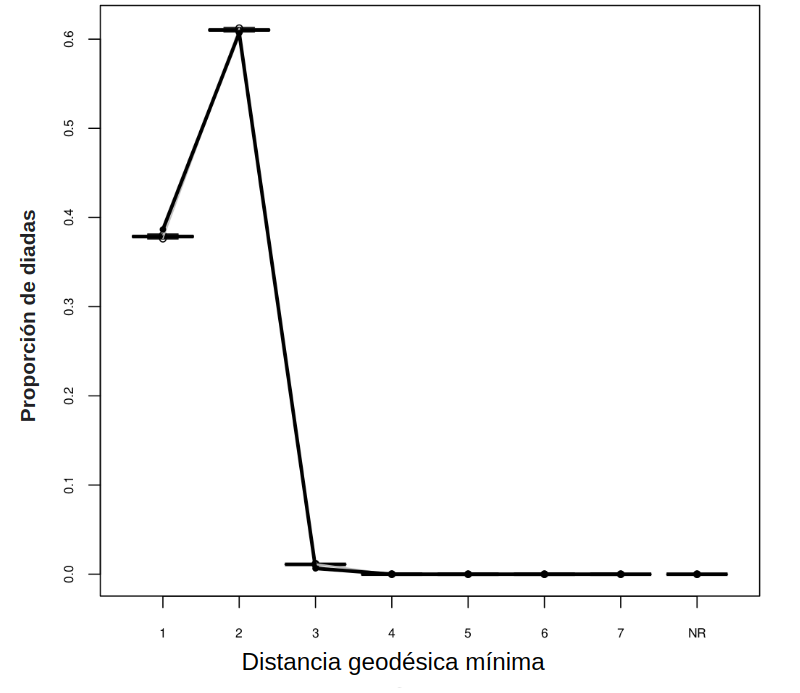
\includegraphics[width=.5\textwidth]{Tesis/Figures/gof_1_distancia.png}
\caption{Medidas de bondad de ajuste del modelo de aristas y Triángulos Estrellas Alternantes}
\end{figure}

De forma adicional también proponemos un modelo en donde podemos incluir información de nuestros nodos con la medida de coincidencia de nodos en temas en general y otro con la especificación de temas en específico cuya clasificación se encuentra en el anexo de esta tesis.

\begin{equation*}
    \textit{Lotame} \sim \textit{Numero.de.Triángulos}+\textit{Estrellas.Alternantes}+
    
    \newline
    \hspace*{2.5cm}\textit{Coincidencia.De.Tema.En.General}
\end{equation*}

y

\begin{equation*}
    \textit{Lotame} \sim \textit{Numero.de.Triángulos}+\textit{Estrellas.Alternantes}+
    
    \newline
    \hspace*{2.5cm} \textit{Coincidencia.De.Tema.En.Específico}
\end{equation*}

cuyos diagnósticos de Markov se encuentran en la Figura 5.16 y 5.17 y cuyos valores de estadísticas son respectivamente $\theta_1 = 125.3$ y $\theta_2 = -124.3$ y $\theta_3 = .5056$ con constante de normalización de $\lambda = .009292$ y $\theta_1 = 16.51799$ y $\theta_2 = -15.22960$ y $\theta_3 = 0.21229$ y cuya constante de normalización es $\lambda = 0.55746$. Vale la pena notar que en el caso de coincidencia de nodos en general las estadísticas de aristas y estrellas alternantes son significativas pero la coincidencia de género en general no lo es. Por el otro lado en el caso de coincidencia de género específico tenemos que las estadísticas de aristas y estrellas alternantes no son significativas pero la de coincidencia de género en específico sí lo es. Además podemos ver que en el caso de la coincidencia de aristas específicas todos los valores de las estadísticas están centradas alrededor de 0. Una interpretación de esto es que utilizando la coincidencia de género especifica nuestro grafo únicamente se conecta utilizando el criterio que sí los nodos comparten el mismo tema en específico o sí es que no. Por el otro lado en el caso en general vemos que parece ser que las estadísticas de aristas y estrellas alternantes determinan la forma en la cual los nodos se conectan mientras que la coincidencia de género únicamente da un poco de forma a la cual nuestro grafo se realiza.

\begin{figure}[!ht]
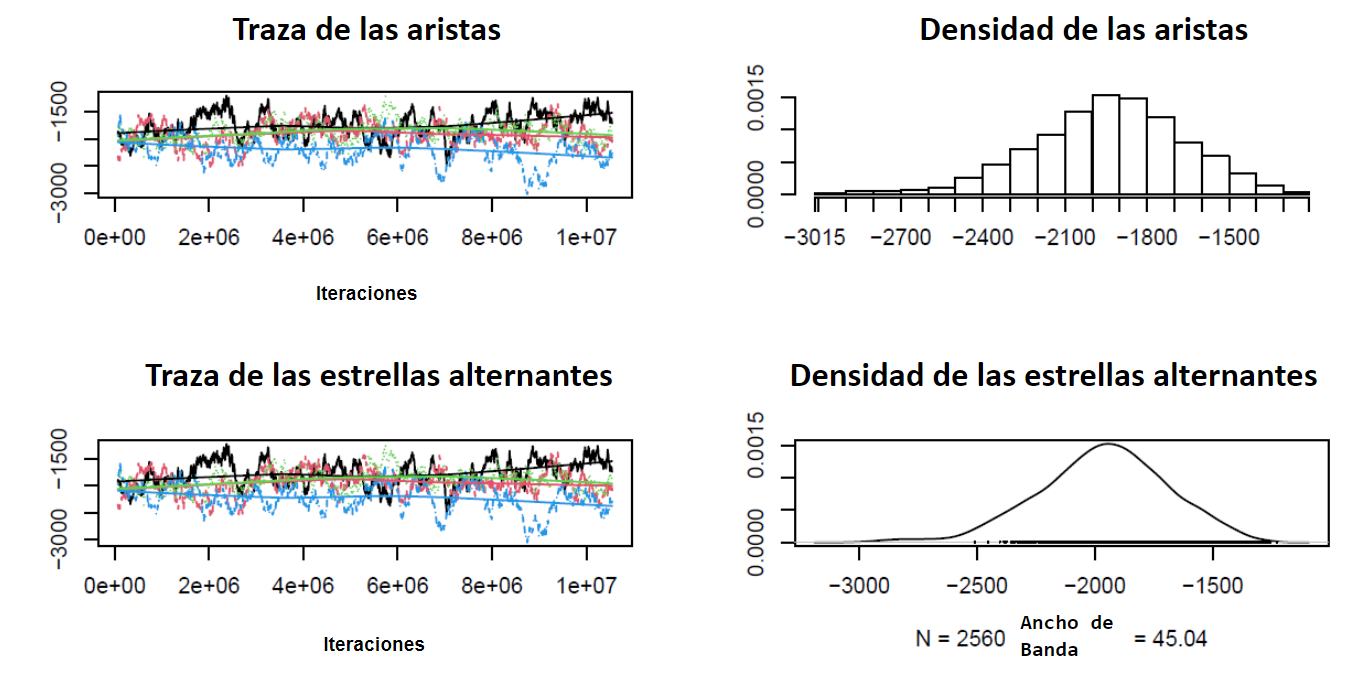
\includegraphics[width=1\textwidth]{Tesis/Figures/mcmc_general1.PNG}
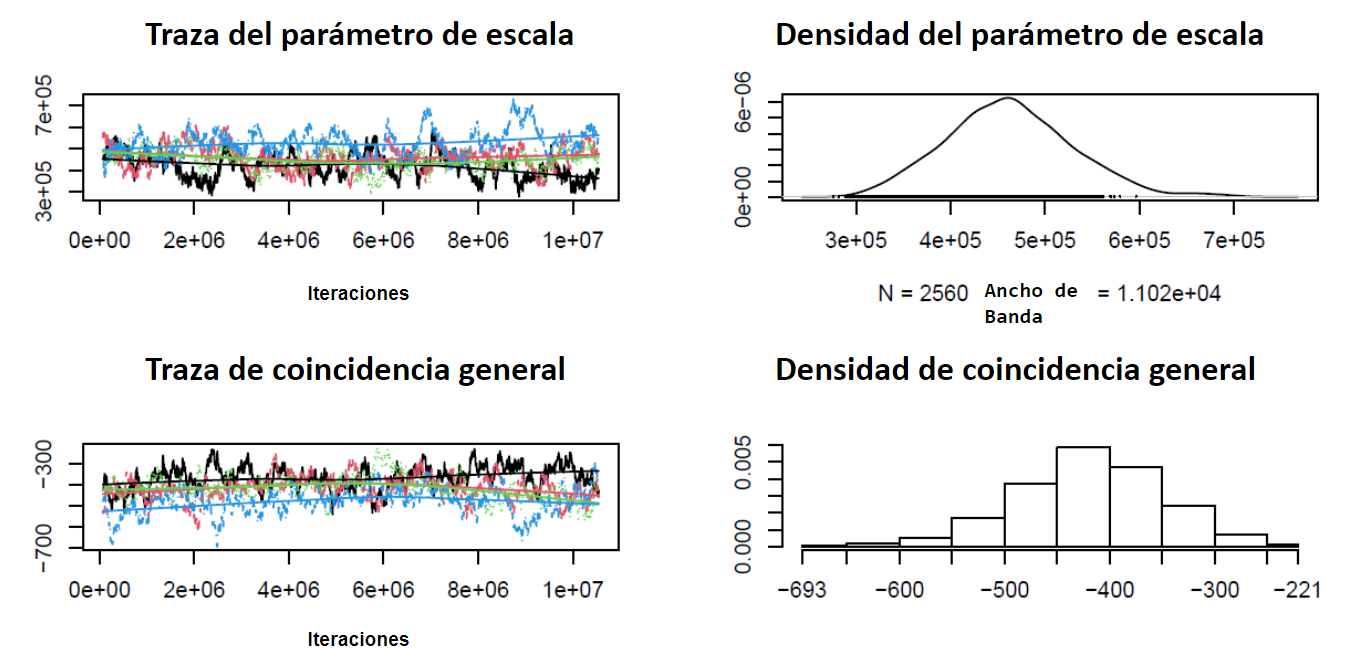
\includegraphics[width=1\textwidth]{Tesis/Figures/mcmc_general2.PNG}
\caption{Diagnósticos de Markov del modelo de Triángulos Estrellas Alternantes y coincidencia de género general}
\end{figure}


\begin{figure}[!ht]
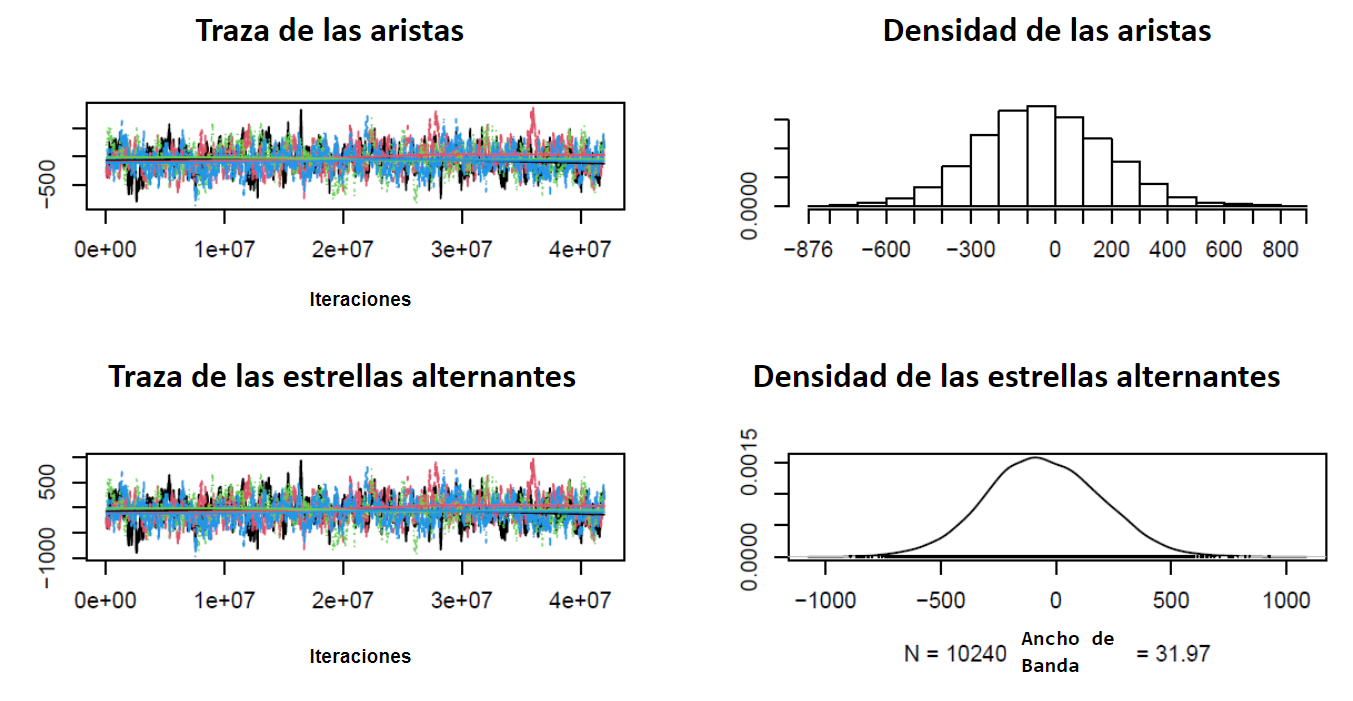
\includegraphics[width=1\textwidth]{Tesis/Figures/mcmc_specific1.PNG}
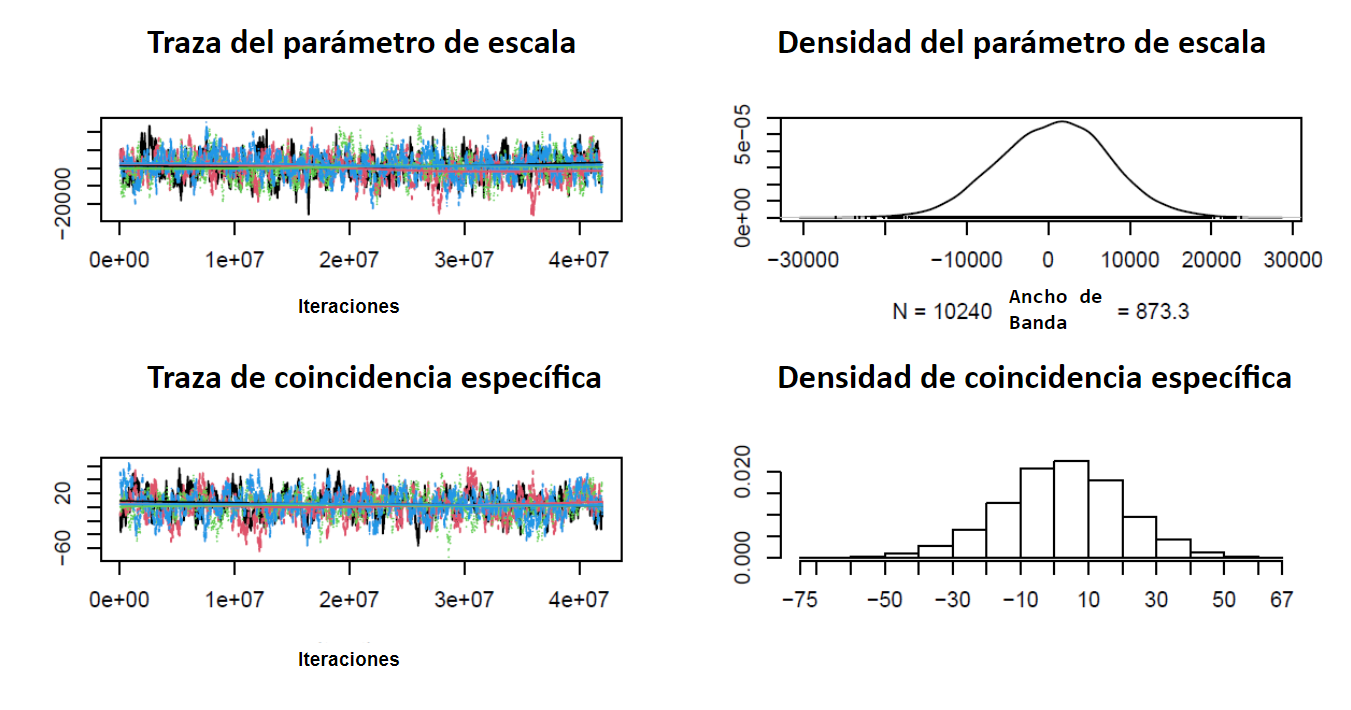
\includegraphics[width=1\textwidth]{Tesis/Figures/mcmc_specific2.PNG}
\caption{Diagnósticos de Markov del modelo de Triángulos Estrellas Alternantes y coincidencia de género específico}
\end{figure}

Viendo las medidas de bondad de ajuste aparentemente se ve mejor el modelo de coincidencia de géneros en específico al menos para la estadística de distancia geodésica. De forma interesante la distribución del grado de los nodos es mayor para el modelo de coincidencia de géneros en específico que para el de coincidencia de géneros en general. Una interpretación es que la coincidencia de género en específico genera comunidades de nodos más interconectados entre sí en donde se tiene grupos más conectados. Más información de estos modelos y sus características se pueden encontrar corriendo el código anexado y disponible en el \textit{github} del anexo.





\begin{figure}[!ht]
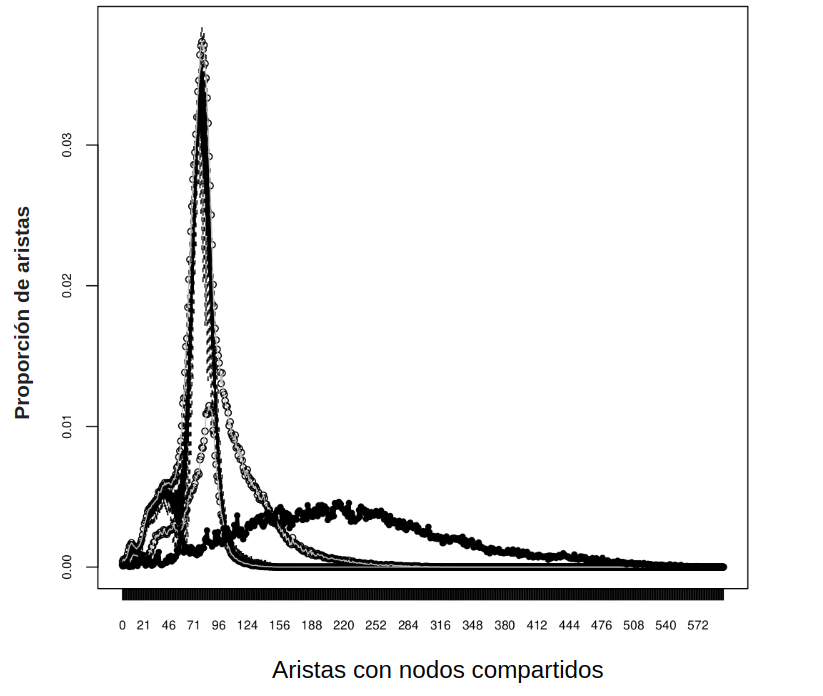
\includegraphics[width=.5\textwidth]{Tesis/Figures/gof_2_aristas_compartidas.png}
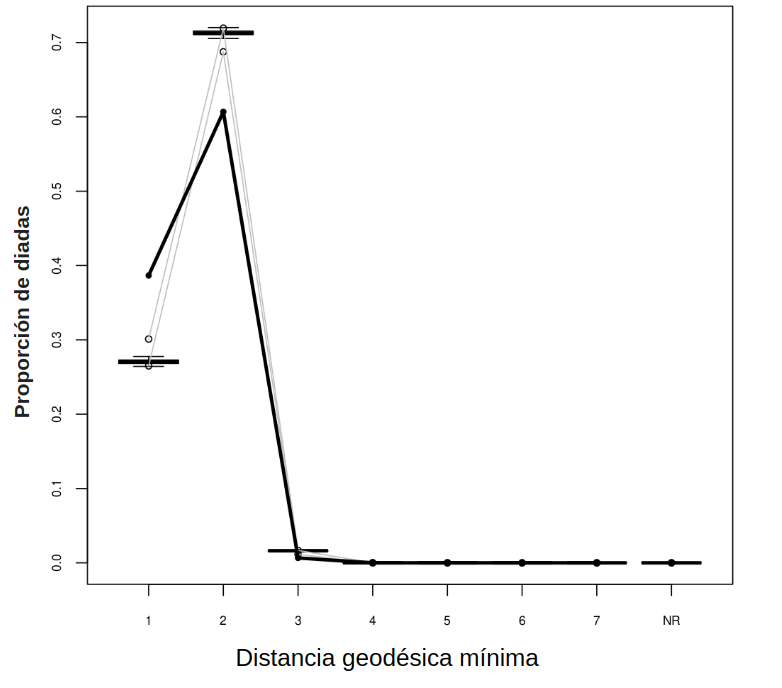
\includegraphics[width=.5\textwidth]{Tesis/Figures/gof_2_distancia.png}
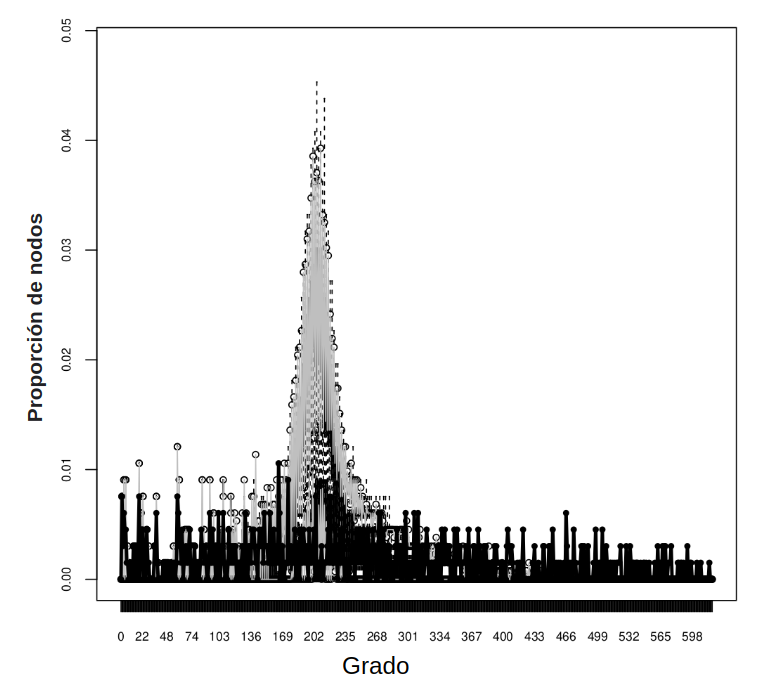
\includegraphics[width=.5\textwidth]{Tesis/Figures/gof_2_grado.png}
\caption{Medidas de bondad de ajuste del modelo de aristas, Triángulos Estrellas Alternantes  y coincidencia de género general}
\end{figure}


\begin{figure}[!ht]
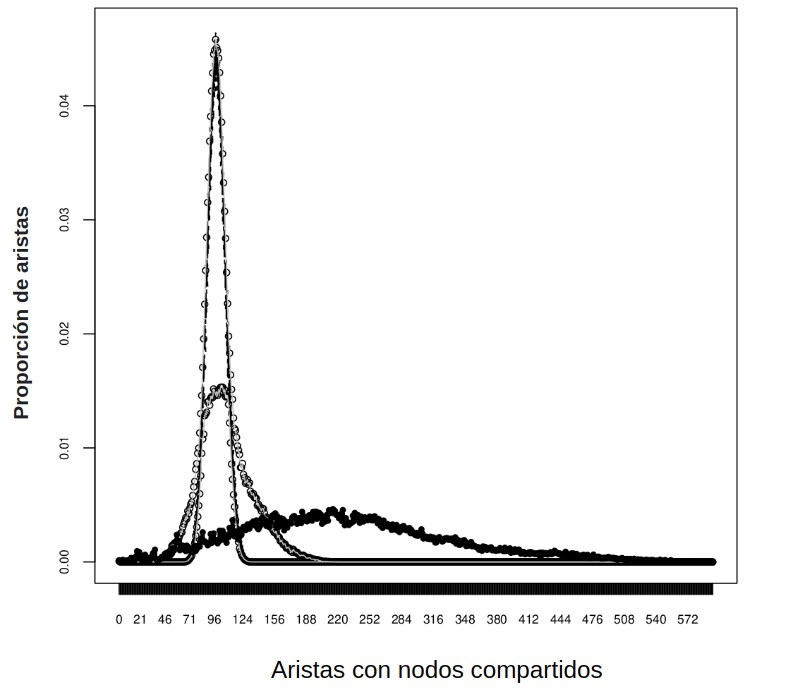
\includegraphics[width=.5\textwidth]{Tesis/Figures/gof_3_aristas_nodos_compartidos.png}
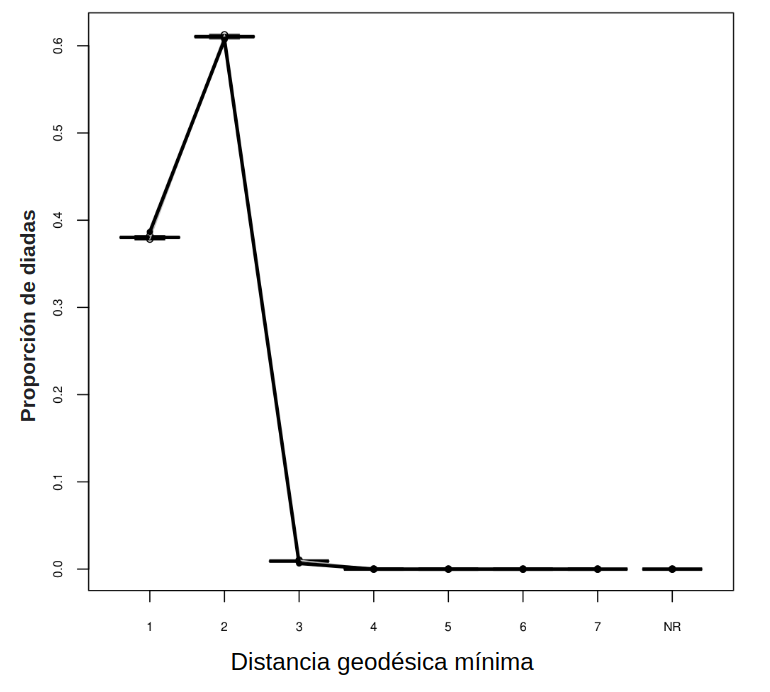
\includegraphics[width=.5\textwidth]{Tesis/Figures/gof_3_distancia.png}
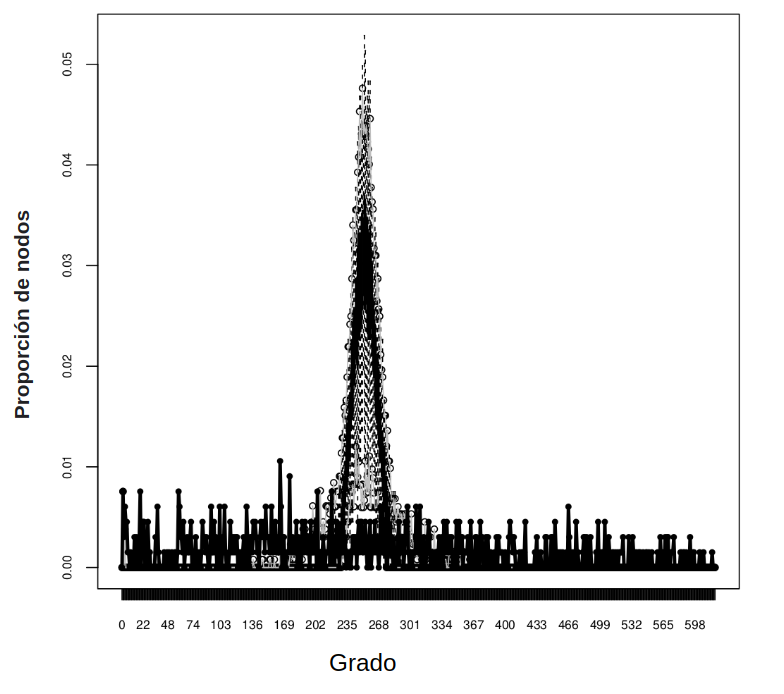
\includegraphics[width=.5\textwidth]{Tesis/Figures/gof_3_grado.png}
\caption{Medidas de bondad de ajuste del modelo de aristas, Triángulos Estrellas Alternantes y coincidencia de género específico}
\end{figure}
    
    \cleardoublepage
    \chapter{Conclusiones}
\label{ch:conclusions}

Los modelos de grafos aleatorias exponenciales son una herramienta más en el repertorio de herramientas de los estadísticos y no son una panacea. Mientras que nos gustaría pensar que podemos usar este tipo de modelos para modelar todo tipo de fenómenos aún tienen muchas limitaciones cuando no tenemos acceso a las estadísticas correctas. Es aún mas difícil encontrar las estadísticas adecuadas cuando nuestros modelos se tardan tiempo aproximadamente infinito en correr.

Sin embargo, esto no debería de ser sorprendente pues estamos intentando encontrar el modelo exponencial que sea capaz de reproducir las propiedades globales de un grafo a través de medidas locales. Además, es importante considerar que en la construcción del modelo es que asumimos por ejemplo en el grafo de amistades que la propensidad de todos nuestros agentes a hacer amigos es la misma a través del grafo, una limitación importante. En el caso empírico de Lotame entonces la inferencia sería que la forma en la que conceptualmente atamos nuestros modelos mentales y las preferencias de distintas audiencias, cada usuario tiene el mismo impacto sobre la composición de esta Grafo de conexiones que el siguiente. Algo que claramente no se cumple pues nuestras aristas se ven construidas de forma que elegimos combinaciones de dos en los n comportamientos de un solo usuario en cualquier momento del tiempo.

Además, la información que contienen estos registros posiblemente se verían mejor modelados con una mezcla de estadísticas temporales y los métodos de Grafos exponenciales valuadas y su uso de la distribución de Conway–Maxwell–Poisson (\cite{TERGMS}). Además de que para llevar a cabo un desarrollo que pueda correr un modelo sobre este gigantesco torrente de información se requeriría un equipo de ingeniería y creatividad como los que trabajan actualmente en Lotame, Hexagon Data o Salesforce. 

Otra dificultad con este problema es sobre poder generar una representación de un `espacio de conocimiento' o intereses que refleje el comportamiento agregado de todos los usuarios en internet. Este conjunto de `nodos platónicos' no es nada trivial. Realmente este problema de simulación y su adyacente problema de conglomerados funcionales podrían eludir nuestros modelos y implementaciones computacionales por un largo tiempo. 

Finalmente, con la muestra que se obtuvo de los datos de las \textit{cookies} en realidad el problema a resolver de encontrar comunidades en internet a partir de las relaciones entre ellas se vuelve trivial si es que simplemente se toman los subgrafos generados del grafo muestreado y se asume que estos subgrafos son en sí las comunidades que estamos buscando. Pues ahora ya no tenemos un interés real en saber las propiedades estadísticas de cada comunidad pues las variables de interés quedan claramente definidas. Una posibilidad para modelar este problema en el futuro sería entonces encontrar los subgrafos de los grafos inducidos a través de periodos temporales discretos y comparar la composición de los subgrafos a través del tiempo utilizando modelos temporales de Grafos aleatorias exponenciales.
 

%%%%%%%%%%%%%%%%%%%%%%%%%%%%%%%%%%%%%%%%%%%%%%
	% APPENDIX
	%%%%%%%%%%%%%%%%%%%%%%%%%%%%%%%%%%%%%%%%%%%%%%
	%\appendix
	 \chapter{Apéndice}
Las funciones para la lectura de las cookies y el muestreo del grafo. El código y los archivos para replicar en parte los resultados de la tesis se encuentran adicionalmente en \href{https://github.com/pdavilab/tesis_ergms}{https://github.com/pdavilab/tesis\_ergms}

Codigo de R para hacer los modelos de \textit{ergm}.

\begin{lstlisting}[language=R]
---
title: "Expanded Lotame ERGM Model"
author: "Patricio Davila"
date: "9/8/2020"
output: html_document
---

```{r, warning=FALSE,echo=FALSE}
#rm(list = ls())
library(tidyverse)
library(statnet)
library(coda)
library(network)
library(sna)
library(network)
library(igraph)
library(intergraph)

```

```{r}

expit <- function(x){
  Things <- exp(x)/(1+exp(x))
  return(Things)
}
library(tidyverse)

RegresaLogOdds <- function(coef,Cuantas){
  #acepta dos para cada argumento 
  #Aristas es una
  #Triangulo es 3
  Factor <- c()
  for(i in seq(coef)){
    FUN <- Cuantas[i]
    #print(FUN)
    Valor <- coef[i]
    #print(Valor)
    Factor[i] <- Valor*FUN
    #print(Probabilidad)
  }
  log_odds <- Factor
  #Probabilidad <- expit(Probabilidad)
  return(log_odds)
}

RegresaProbabilidad <- function(log_odds){
  log_odds <- sum(log_odds)
  Thing <- expit(log_odds)
  return(Thing)
}



FuncionAcumulada <- function(Coefs,Cambio){
  IndexSave2 <- list()
IndexSave <- list()


for(i in seq(100)){
  logOddsFlorentino <- RegresaLogOdds(c(Coefs),
  c(Cambio,i-1))
  logOddsFlorentino
ProbabilidadFlorentina <- RegresaProbabilidad
(logOddsFlorentino)
ProbabilidadFlorentina
  IndexSave2[i] <- list(logOddsFlorentino)
  IndexSave[i] <- ProbabilidadFlorentina
}

  return(list(IndexSave2,IndexSave))
}  


```

```{r}
MasterTable <- read.csv(
    "WeightedExpandedReplacedEdgelist.csv")
#The 5701 classified taxonomy elements
Taxonomy <- read.csv("TaxonomyMain.csv")

#CustomTaxonomy
Nodes <-  Taxonomy %>% 
as.tibble() %>%
mutate(node_id = seq(
1:length(Taxonomy$Node_ID))) %>% 
#separate(Node_Name,
into = paste0(seq(1:10)),sep="[^]") %>% 
mutate(Node_Name = 
str_replace(Node_Name,"-","[^]"))

LDXShopping <- dplyr::filter(Nodes, 
grepl('Shopping|Retail|Market|Gift|Purchase',
`Node_Name`))

LDXCategory <- dplyr::filter(Nodes, grepl(
'Lotame Category Hierarchy', `Node_Name`))

NodeList <- rbind(LDXShopping,LDXCategory) %>% 
unique()
#just making sure all of 
our edgelist elements are 
in any of the 2483 nodes 
of the two original 
chosen taxonomies
Mastaa <- MasterTable %>% 
  inner_join(select(NodeList, Node_ID),
  by=c("To"="Node_ID")) %>% 
  inner_join(select(NodeList, Node_ID), 
  by=c("From"="Node_ID")) %>% 
  rename(
    from = From,
    to = To
    )


```

```{r}

NodesX <- read.csv(
"node_level_data_Shorthand_Reducido.csv")


#Add removing Factor level five.

Nodes <- NodesX %>% 
  #select(-c(Arbol_8)) %>% 
  #select(-c(Arbol_7)) %>% 
  #select(-c(Arbol_6)) %>% 
  #select(-c(Arbol_5)) %>% 
  #group_by(To, From,ToId,FromId) %>% 
  #summarise(weight = n()) %>% 
  ungroup() %>% 
  mutate(Node_ID = as.factor(Node_ID))

NewNodeList <- NodesX %>% 
  filter(Node_ID == NEWID) %>% 
  #select(-c(Arbol_8)) %>% 
  #select(-c(Arbol_7)) %>% 
  #select(-c(Arbol_6)) %>% 
  #select(-c(Arbol_5)) %>% 
  #group_by(To, From,ToId,FromId) %>% 
  #summarise(weight = n()) %>% 
  ungroup() %>% 
  mutate(Node_ID = as.factor(Node_ID)) %>% 
  mutate(Node_ID = as.character(Node_ID)) %>% 
  mutate(NEWID = as.character(NEWID))


EdgeFin <- Mastaa %>% 
  filter(as.character(from) %in% 
  NewNodeList$NEWID) %>% 
  filter(as.character(to) %in% 
  NewNodeList$NEWID)

EdgeFin <- EdgeFin %>% 
  group_by(to, from) %>% 
  filter(to != from) %>% 
  summarise(weight= sum(freq)) %>%
  ungroup() %>% 
  filter(from %in% NewNodeList$NEWID) %>% 
  filter(to %in% NewNodeList$NEWID)

net <- igraph::graph_from_data_frame(d = EdgeFin, 
vertices = NewNodeList,directed = FALSE)

directed_graph_wgt <- graph.data.frame(EdgeFin, 
directed = TRUE, vertices = NewNodeList)
undirected_graph_wgt <- as.undirected(
directed_graph_wgt, mode = "collapse",
edge.attr.comb = "sum")


```
```{r}

set.seed(141719)
Empieza <- asNetwork(undirected_graph_wgt)
#summary(Empieza)
#Modelling
#save(Empieza, file = "stuff.RData")
l <- layout_on_sphere(net)
l2 <- layout_with_fr(net)
V(net)$size <- 8
colrs <- sample(colors(),45)
V(net)$frame.color <- "black"
V(net)$group_id <- as_tibble(
V(net)$ShortName_General) %>% 
group_by(value)%>% group_indices(value) 
V(net)$color <- colrs[V(net)$group_id]
V(net)$label <- "" 
E(net)$arrow.mode <- 0
plot(net, vertex.cex=.05,
vertex.label=NA,layout=l2)

```

```{r}
#Quantile 20 cut off

cutoff <- quantile(EdgeFin$weight)
EdgeFinR <- EdgeFin %>% 
  filter(as.numeric(weight) >= 46)

net <- igraph::graph_from_data_frame(
d = EdgeFinR, 
vertices = NewNodeList,directed = FALSE)

directed_graph_wgt <- graph.data.frame(
EdgeFinR, directed = TRUE, 
vertices = NewNodeList)
undirected_graph_wgt <- as.undirected(
directed_graph_wgt, mode = "collapse",
edge.attr.comb = "sum")

components <- igraph::
clusters(undirected_graph_wgt, 
mode="weak")
biggest_cluster_id <- 
which.max(components$csize)

# ids
vert_ids <- V(undirected_graph_wgt)
[components$membership == 
biggest_cluster_id]

# subgraph
biggestC <- igraph::induced_subgraph(
undirected_graph_wgt, vert_ids)
Empieza2 <- asNetwork(biggestC)


max_subgraph_graph <- biggestC
Empieza <- asNetwork(biggestC)

logweight <- EdgeFin %>% 
mutate(log_wg = log(weight)) %>%
.$log_wg
hist (logweight,
main="Histograma de los 
log peso del grafo completo",
xlab="Valor de los log peso",
border="Chocolate2",
col="pink",
las=2,
breaks=75,
prob = TRUE)


EdgeFinR %>% mutate(log_wg = log(weight)) %>% 
.$log_wg %>%
hist (logweight,
main="Histograma de 
los log peso del subgrafo inducido",
xlab="Valor de los log peso",
border="Chocolate2",
col="pink",
las=2,
breaks=75,
prob = TRUE)

library(RColorBrewer)
set.seed(14119)
l <- layout_on_sphere(max_subgraph_graph)
l <- layout_with_fr(max_subgraph_graph)
V(max_subgraph_graph)$size <- 8
colrs <- sample(colors(),45)
V(max_subgraph_graph)$frame.color <- "white"
V(max_subgraph_graph)$group_id <- as_tibble(
V(max_subgraph_graph)$ShortName_General) %>% 
group_by(value)%>% group_indices(value) 
V(max_subgraph_graph)$color <- 
colrs[V(max_subgraph_graph)$group_id]
V(max_subgraph_graph)$label <- ""
E(max_subgraph_graph)$arrow.mode <- 0
l <- layout_in_circle(max_subgraph_graph)
plot(max_subgraph_graph,layout=l)
```




```{r,eval=FALSE}
max_subgraph <- max_cliques(
max_subgraph_graph, min = NULL, 
max = NULL, subset = NULL,
  file = NULL)

max = 0
for (i in seq(length(max_subgraph))){
  size = length(max_subgraph[[i]])
  if(size > max){
    max = size
    index = i
  }
}

max_subgraph_graph <- induced_subgraph(
  max_subgraph_graph,
  max_subgraph[[index]]
)
Empieza <- asNetwork(max_subgraph_graph)
```
```{r,eval=FALSE}
library(RColorBrewer)
set.seed(141719)
l <- layout_on_sphere(max_subgraph_graph)
l <- layout_with_fr(max_subgraph_graph)
V(max_subgraph_graph)$size <- 8
colrs <- sample(colors(),45)
V(max_subgraph_graph)$frame.color <- "white"
V(max_subgraph_graph)$group_id <- as_tibble(
V(max_subgraph_graph)$ShortName_General) %>% 
group_by(value)%>% group_indices(value) 
V(max_subgraph_graph)$color <- 
colrs[V(max_subgraph_graph)$group_id]
V(max_subgraph_graph)$label <- "" 
E(max_subgraph_graph)$arrow.mode <- 0
plot(max_subgraph_graph,layout=l)
```


```{r}
set.seed(141719)
#-3.2598822  0.0216762
#-3.2603808,0.0216776
#-3.26104824  0.02167921 
#-3.26154720  0.02168062 
edge_triangleF <- ergm(Empieza2~edges+triangles,
control = control.ergm(seed=141719,
init = c(-3.26154720 ,0.02168062),
MCMLE.maxit = 1,MCMC.samplesize=10240
,MCMC.interval=4096,parallel =4,
parallel.type="PSOCK"),
control.SAN = control.san(SAN.maxit = 800, 
SAN.tau = 1, SAN.invcov = NULL,
SAN.invcov.diag = FALSE, 
SAN.nsteps.alloc = function(nsim)
4^seq_len(nsim), SAN.nsteps = 4^19, 
SAN.samplesize =84^12,
SAN.init.maxedges = 20000, 
SAN.max.maxedges = 2^26,
SAN.prop.weights = "default", 
SAN.prop.args = list(),
SAN.packagenames = c(), 
term.options = list(), seed = NULL,
parallel = 0, parallel.type = NULL, 
parallel.version.check = TRUE),
verbose=T)

# 16.5167         -15.2282           
0.5574 
edges_alt_kF <- ergm(Empieza2~
edges+altkstar(1, fixed=FALSE),
control = control.ergm(seed=141719,
MCMC.samplesize=10240,
MCMC.interval=4096,parallel=4,
parallel.type="PSOCK"),
verbose=T)

# edges                     
altkstar         
altkstar.lambda  
#                   15.77352                
-14.65663                 
0.55356  
#nodematch.ShortName_General  
#                   -0.09923  
edges_alt_k_generalF <- ergm(Empieza2~
edges+altkstar(0.55356, fixed=FALSE)+
nodematch("ShortName_General"),
control = control.ergm(seed=141719,
init = c(15.77352,-14.65663,-0.09923),
MCMC.samplesize=10240,MCMC.interval=4096,
parallel=4,
parallel.type="PSOCK"),
verbose=T)

edges_only <- ergm(Empieza2~edges,
control = control.ergm(seed=141719,
parallel=4,
parallel.type="PSOCK"),
verbose=T)

edges_alt_k_specificF <- ergm(Empieza2~
edges+altkstar(1, fixed=FALSE)+
nodematch("ShortName_Specific"),
control = control.ergm(
seed=141719,MCMC.samplesize=10240,
MCMC.interval=4096,parallel=4,
parallel.type="PSOCK"),
verbose=T)
#########################MODEL 1##############

name <- "edge_triangle3"
model <- edge_triangleF

#alt_k_edge_model
  
summary(model)
pdf(paste('mcmc_diagnostics',name,'.pdf'))
mcmc.diagnostics(model)
dev.off() 


######################MODEL2####################


name <- "edges_alt_kF3"
model <- edges_alt_kF

#alt_k_edge_model
  
summary(model)
pdf(paste('mcmc_diagnostics',name,'.pdf'))
mcmc.diagnostics(model)
dev.off() 



###########################Model 3 ###########

name <- "edges_alt_k_generalF3"
model <- edges_alt_k_generalF

#alt_k_edge_model
  
summary(model)
pdf(paste('mcmc_diagnostics',name,'.pdf'))
mcmc.diagnostics(model)
dev.off()

#################Model 4###############

name <- "edges_alt_k_specificF3"
model <- edges_alt_k_specificF

#alt_k_edge_model
  
summary(model)
pdf(paste('mcmc_diagnostics',name,'.pdf'))
mcmc.diagnostics(model)
dev.off()
```

```{r}
summary(edge_triangleF)
summary(edges_alt_kF)
summary(edges_alt_k_generalF)
summary(edges_alt_k_specificF)
```

```{r,eval=FALSE}
#Lotame.01.gof <- gof(edge_triangleF~
degree + esp + distance, 
control.gof.formula(nsim=10))
Lotame.02.gof <- gof(edges_alt_kF~degree 
+ esp + distance, 
control.gof.formula(nsim=10))
Lotame.03.gof <- gof(edges_alt_k_generalF~
degree + 
esp + distance, 
control.gof.formula(nsim=10))
Lotame.04.gof <- gof(edges_alt_k_specificF~
degree + 
esp + distance, 
control.gof.formula(nsim=10))
```


```{r,eval=FALSE}
#plot(Lotame.01.gof)

summary(model)
pdf(paste('GOF ALL',"Aca",'.pdf'))
plot(Lotame.02.gof)
plot(Lotame.03.gof)
plot(Lotame.04.gof)
dev.off()

```

```{r,eval=FALSE}
Lotame.01.sim <- simulate(edge_triangleF,
nsim=10)
rbind("obs"=summary(edge_triangleF),
"sim mean"=
colMeans(attr(Lotame.01.sim, "stats")))

Lotame.02.sim <- simulate(edges_alt_kF,nsim=10)
rbind("obs"=summary(edges_alt_kF),
"sim mean"=colMeans(attr(Lotame.02.sim, "stats")))

Lotame.03.sim <- simulate(edges_alt_k_generalF,
nsim=10)
rbind("obs"=summary(edges_alt_k_generalF),
"sim mean"=colMeans(attr(Lotame.03.sim, "stats")))

Lotame.04.sim <- simulate(edges_alt_k_specificF,
nsim=10)
rbind("obs"=summary(edges_alt_k_specificF),
"sim mean"=colMeans(attr(Lotame.04.sim, "stats")))
```


```{r,eval=FALSE}

model1sim <- asIgraph(Lotame.01.sim[[1]])

net <- Lotame.01.sim[[1]]
l2 <- layout_with_fr(net)
V(net)$size <- 8
colrs <- sample(colors(),45)
V(net)$frame.color <- "black"
V(net)$group_id <- as_tibble(
V(net)$ShortName_General) %>% 
group_by(value)%>% group_indices(value) 
V(net)$color <- colrs[V(net)$group_id]
V(net)$label <- "" 
E(net)$arrow.mode <- 0

plot(Lotame.01.sim[[1]], 
 label= Lotame.01.sim[[1]] %v%
 "ShortName_General",
 vertex.cex = .25,layout=l2)

model2sim <- asIgraph(Lotame.02.sim[[1]])

net <- Lotame.02.sim[[1]]
l2 <- layout_with_fr(net)
V(net)$size <- 8
colrs <- sample(colors(),45)
V(net)$frame.color <- "black"
V(net)$group_id <- as_tibble(
V(net)$ShortName_General) %>% 
group_by(value)%>% group_indices(value) 
V(net)$color <- colrs[V(net)$group_id]
V(net)$label <- "" 
E(net)$arrow.mode <- 0

plot(Lotame.02.sim[[1]], 
 label= Lotame.02.sim[[1]]
 %v% "ShortName_General",
 vertex.cex = .25,layout=l)

model3sim <- asIgraph(
Lotame.03.sim[[1]])

net <- Lotame.03.sim[[1]]
l2 <- layout_with_fr(net)
V(net)$size <- 8
colrs <- sample(colors(),45)
V(net)$frame.color <- "black"
V(net)$group_id <- as_tibble(
V(net)$ShortName_General) %>%
group_by(value)%>% group_indices(value) 
V(net)$color <- colrs[V(net)$group_id]
V(net)$label <- "" 
E(net)$arrow.mode <- 0

plot(Lotame.03.sim[[1]], 
 label= Lotame.03.sim[[1]] %v% 
 "ShortName_General",
 vertex.cex = .25,layout=l)

model4sim <- asIgraph(Lotame.04.sim[[1]])

net <- Lotame.04.sim[[1]]
l2 <- layout_with_fr(net)
V(net)$size <- 8
colrs <- sample(colors(),45)
V(net)$frame.color <- "black"
V(net)$group_id <- as_tibble(
V(net)$ShortName_General) %>% 
group_by(value)%>% group_indices(value) 
V(net)$color <- colrs[V(net)$group_id]
V(net)$label <- "" 
E(net)$arrow.mode <- 0

plot(Lotame.04.sim[[1]], 
label= Lotame.04.sim[[1]] 
%v% "ShortName_General",
vertex.cex = .25,layout=l)
```





\end{lstlisting}

Codigo de python para leer las cookies y hacer nuestro \textit{edgelist}.

\begin{lstlisting}[language=Python]
# %%
import json
import pandas as pd
import itertools
import ast
from pandas.io.json import json_normalize 
import os
import ast
import numpy as np
import gzip
import shutil

def Read_Cookies(filenames,stop_max=False):
looperino = 1
with open(filenames,"r",encoding="UTF-8", 
errors="ignore") as in_file:
dicts = []
for line in in_file.readlines(): 
    d = json.loads(line.strip())
    dicts += [d]
    looperino = looperino +1
if (looperino > 2500) and (stop_max == True):
    break
return(dicts)

#Get mappiings
def get_dictionary_mappings():
with open('mappings.json',"r",
encoding="UTF-8",errors = 'ignore')as infile:
    mappings = []
    for line in infile.readlines(): 
        d = json.loads(line.strip())
        mappings += [d]
mappper=[]
for map in mappings:
    beh_id = map['behavior_id']
    hierarchy_nodes = map['hierarchy_nodes']
    for hierarchy in hierarchy_nodes:
    mappper.append((
    beh_id,hierarchy['id'],hierarchy['path']))

df = pd.DataFrame(mappper, columns=
['beh_id','tax_id',
"path_id"])
diccionario_relevante = df[["beh_id","tax_id"]]
diccionario_relevante = diccionario_relevante.
astype(int)
diccionario_relevante = diccionario_relevante.
astype(str)
# diccionario_relevante = diccionario_relevante.
select_dtypes(include='str')
diccionario_relevante_dict = diccionario_relevante.
set_index('beh_id').to_dict()['tax_id']
return(diccionario_relevante_dict)

diccionario_relevante_dict = get_dictionary_mappings()

def replace_id_beh_for_taxonomy_node():
working_df = pd.read_csv("WeightedEdgelist.csv")
working_df = working_df.loc[:,
~working_df.columns.str.contains('^Unnamed')]
working_df = working_df.astype(int)
working_df = working_df.astype(str)
# work = working_df.select_dtypes(include='str')
i=0
fails = pd.DataFrame()
table = pd.DataFrame()
for chunk in np.array_split(working_df, 250):
print(i)
try:
chunkerino = chunk.replace({'
To':diccionario_relevante_dict})
chunkerino = chunkerino.replace(
{'From':diccionario_relevante_dict})
table = pd.concat([table,chunkerino])
except TypeError as identifier:
print("failed at",i)
fails = pd.concat([fails,chunk])
pass
i = i+1
table = table[table['To'] != table['From']]
# table = table.to_csv('replacededgelist_aux.csv')
return table

def reduce_total_taxonomy_
edgelist_to_category_shopping_taxonomy(
table,diccionario_relevante_dict):
reducido = pd.read_csv(
"FolderAsesorSinodal/node_level_data_
Shorthand_Reducido.csv").dropna()
tablenew = table.loc[table['To'].isin(
list(reducido['Node_ID']))]
tablenew = tablenew.loc[table['From'].isin(
list(reducido['Node_ID']))]
diccionario_relevante = reducido[["Node_ID","NEWID"]]
diccionario_relevante = diccionario_relevante.
astype(int)
diccionario_relevante = diccionario_relevante.
astype(str)
# diccionario_relevante = diccionario_relevante.
select_dtypes(include='str')
diccionario_relevante_dict = diccionario_relevante.
set_index('Node_ID').to_dict()['NEWID']
final_table = tablenew.replace(
{'To':diccionario_relevante_dict})
final_table = final_table.replace(
{'From':diccionario_relevante_dict}).
groupby(["To","From"]).sum().reset_index()
final_table = final_table.loc[:,
~final_table.columns.str.contains('^Unnamed')]
final_table.to_csv("
WeightedExpandedReplacedEdgelist.csv",
index=False)
return(final_table)


def get_file_type(filepath,typerino):
all_files = []
for root, dirs, files in os.walk(filepath):
    files = glob.glob(os.path.join(root,'*'+typerino))
    for f in files :
        all_files.append(os.path.abspath(f))
return all_files


def CreateHierarchyEdgelist_optim(
dicts,filename):
# import ast
iter = 0
Listed = []
Listed2 = []
ListOfLists = []
ListOfLists2 = []
TimeStampList = []
InnerIter = 1
for record in dicts:
events = record['events'][0]
if 'add' in events.keys():
TimeStamp = events['ts']
EventList = events['add']
else:
TimeStamp = events['ts']
EventList = events['remove']
Listed = []
Listed2 = []
for happen in EventList:
DataF = Taxonomy[Taxonomy[
'behavior_id'] == happen]
if DataF.empty:
NADA = "Nada"
else:
for i in range(len(DataF)):
    Hier = Taxonomy[Taxonomy
    ['behavior_id'] == happen].
    reset_index()['behavior_id'][i]
    Hier = str(Hier)
    Listed.append(Hier)
ListOfLists.append(list(
pd.Series(Listed, name='A')
.unique()))
ListOfLists2.append(Listed2)
TimeStampList.append(TimeStamp)
iter = iter + 1
if iter % 50 ==0: 
a = ListOfLists
a2 = ListOfLists2
Edges = []
EdgesTax = []
TimeAuxList = []
for i in range(len(ListOfLists)):
if len(ListOfLists[i]) > 50:
    ListOfLists[i] = ListOfLists[i][0:50]
h = itertools.combinations(ListOfLists[i], 2)
TimeAux = TimeStampList[i]
for comb in h:
    Edges.append(comb)
    TimeAuxList.append(TimeAux)
for lists in a2:
if len(lists) > 50:
    lists = lists[0:50]
h2 = itertools.combinations(lists,2)
Edges = pd.DataFrame(Edges, columns = ["To","From"])
TimeAuxList = pd.DataFrame(TimeAuxList,
columns= ['TimeStamp'])
Edges = pd.concat([Edges.reset_index(drop=True),
TimeAuxList],axis=1)
Edges.to_csv(str(filename)+ "_" 
+str(InnerIter)+".csv")
InnerIter = InnerIter + 1
print(InnerIter*50/len(dicts),
"percentage of task done")
if iter % 50 ==0:
Listed = []
Listed2 = []
ListOfLists = []
ListOfLists2 = []
TimeStampList = []
if iter % len(dicts) == 0:
a = ListOfLists
a2 = ListOfLists2
Edges = []
EdgesTax = []
TimeAuxList = []
for i in range(len(ListOfLists)):
    if len(ListOfLists[i]) > 50:
        ListOfLists[i] = ListOfLists[i][0:50]
    h = itertools.combinations(ListOfLists[i], 2)
    TimeAux = TimeStampList[i]
    for comb in h:
        Edges.append(comb)
        TimeAuxList.append(TimeAux)
for lists in a2:
    if len(lists) > 50:
        lists = lists[0:50]
    h2 = itertools.combinations(lists,2)
Edges = pd.DataFrame(Edges, 
columns = ["To","From"])
TimeAuxList = pd.DataFrame(TimeAuxList, 
columns= ['TimeStamp'])
Edges = pd.concat([Edges.reset_index(drop=True),
TimeAuxList],axis=1)
Edges.to_csv(str(filename)+ "_" 
+str(InnerIter)+".csv")
Inneriter = InnerIter + 1
print(InnerIter*50/len(dicts),
"percentage of task done")
print("Finished")

def master_sampler():
GZIPdirectory = 'E:/Data & Thesis/DataStreamZIPDUMP'
gzips_location = get_file_type(GZIPdirectory,'.gz')
list_of_stop_words = ["Edges", "Florentine", 
"mappings.json.gz","TaxonomyMain.csv"]
filtered_str = [x for x in gzips_location 
if x not in set(list_of_stop_words)]
i = 1
weighted_edge_list = pd.DataFrame()
weighted_edge_list.to_csv("WeightedEdgelist.csv")
donefiles = []
try:
os.mkdir('Auxfiles') 
except OSError as e:
print("Ya esta el directorio")
for file in filtered_str:
fp = open("zen1.txt", "wb")
with gzip.open(file,'rb') as f:
data = f.read()
fp.write(data)
fp.close()
dicts = Read_Cookies("zen1.txt")
CreateHierarchyEdgelist_optim(dicts,"Auxfiles/aux")
j = 0
aux_files = get_file_type(
"Auxfiles",'.csv')
weighted_edge_list = pd.read_csv(
"WeightedEdgelist.csv")
weighted_edge_list = weighted_edge_list.loc[:,
~weighted_edge_list.columns.str.
contains('^Unnamed')]
for auxs in aux_files:
Thing = pd.read_csv(auxs)
if len(Thing)>0:
    max_batch = max(Thing['TimeStamp'])
    min_batch = min(Thing['TimeStamp'])
    Thing = Thing[['To','From']]
    Thing['freq']=Thing.groupby(by=['To'])
    [['To']].transform('count')
    Thing = Thing[Thing['To'] != Thing['From']]
    weighted_edge_list = pd.concat(
    [Thing,weighted_edge_list]).groupby(
    ["To","From"]).
    sum().reset_index()
    j = j +1
    print(j/len(aux_files),"Appending done")
try:
shutil.rmtree('Auxfiles')
except OSError as e:
print ("Error: %s - %s." %
(e.filename, e.strerror))
try:
os.mkdir('Auxfiles') 
except OSError as e:
print("Ya esta el directorio")
pass
print(i*100/len(filtered_str),
"PERCENTAGE OF GZ FILES DONE")
donefiles.append(file)
i = i+1
fp = open("gzips.txt", "wb")
fp.write(donefiles)
fp.close()
return(donefiles)
# %%
def check_time_logs():
with open('gzips.txt',"r",encoding="utf-8",
errors="ignore") as in_file:
dicts = []
for line in in_file.readlines():
    line = line.replace('\\','/')
    line = line.replace('\n','')
    dicts += [line]
min_time = 1536486306
max_time = 1536486306 
#First observation of the cookies
cookies = 0
iter2 = 0
total = 0
for file in dicts:
size = os.path.getsize(file)
total = total + size
for file in dicts:
fp = open("zen1.txt", "wb")
with gzip.open(file,'rb') as f:
data = f.read()
fp.write(data)
fp.close()
dictss = Read_Cookies("zen1.txt")
for dicty in dictss:
time = dicty['events'][0]['ts']
if time < min_time:
    min_time=time
if time > max_time:
    max_time = time
print(min_time,max_time)
iter2 = iter2 +1
cookies = cookies + len(dictss)
print(iter2/len(dicts))
#max_time de la muestra es: 1537286399
#min_time de la muestra es: 1536267600
#numero de registros de cookies: 25435675
return(max_time,min_time,total)

\end{lstlisting}


	%%%%%%%%%%%%%%%%%%%%%%%%%%%%%%%%%%%%%%%%%%%%%%
	% BIBLIOGRAPHY
	%%%%%%%%%%%%%%%%%%%%%%%%%%%%%%%%%%%%%%%%%%%%%%
	\clearpage
	\addcontentsline{toc}{chapter}{Bibliografía} %Añadimos la bibliografia a la lista de contenidos.
	
	%%%%%%%%% Referencias usando el sistema embebido %%%%%%%%%%%
	% e.g. (Ejemplo tomado de https://en.wikibooks.org/wiki/LaTeX/Bibliography_Management)
	%
	% \begin{thebibliography}{9}
	%
	%	\bibitem{lamport94}
    %			Leslie Lamport,
    %			\emph{LaTeX: a document preparation system},
    %			Addison Wesley, Massachusetts,
  	%			2nd edition,
    % 			1994.
    %
	% \end{thebibliography}

	%%%%%%%%% Referencias usando bibtex %%%%%%%%%%%
    %--------------------------------------------------------------------------------
%   BIBLIOGRAFÍA
%--------------------------------------------------------------------------------

\backmatter
\nocite{*}
% \bibliographystyle{apacite}
\bibliographystyle{agsm}
% \bibliography{EVRWedit}
\bibliography{references}
%\bibliographystyle{apacite} % Así se usa y cols. en lugar de et al.
%bibliographystyle{plainnat}
%\bibliography{references.bib}
% \printbibliography
    %\renewcommand{\bibname}{References}
	%\bibliographystyle{unsrt}
	%\bibliography{references} 



\end{document}